\subsection*{Lisenssi 
\includegraphics[scale=0.3]{pictures/cc.pdf} 
\includegraphics[scale=0.3]{pictures/by.pdf}}

Tämän teoksen käyttöoikeutta koskee Creative Commons Nimeä 3.0 Muokkaamaton (CC BY 3.0) -lisenssi.
This work is licensed under a Creative Commons Attribution 3.0 Unported (CC BY 3.0) License.

\qrlinkki{http://creativecommons.org/licenses/by/3.0/deed.fi}{Lisenssin suomenkielinen tiivistelmä}
\qrlinkki{http://creativecommons.org/licenses/by/3.0/deed.en}{Lisenssin englanninkielinen tiivistelmä}
\qrlinkki{http://creativecommons.org/licenses/by/3.0/legalcode}{Tarkat lisenssiehdot (englanniksi)}

Sinulla on vapaus:
\begin{enumerate}
\item jakaa — kopioida, levittää, näyttää ja esittää teosta
\item remiksata — valmistaa muutettuja teoksia
\item käyttää teosta kaupallisiin tarkoituksiin
\end{enumerate}
Seuraavilla ehdoilla:
\begin{enumerate}
\item nimeä — Teoksen tekijä on ilmoitettava siten kuin tekijä tai teoksen lisensoija on sen määrännyt (mutta ei siten että ilmoitus viittaisi lisenssinantajan tukevan lisenssinsaajaa tai Teoksen käyttötapaa)
\end{enumerate}

Määräys lisäyksenä lisenssiin: kaikkien kirjoittajien nimet on ilmoitettava jossakin kohtaa kirjaa.



\newpage
\subsection*{Kirjoittajat}
\begin{itemize}
\item Lauri Hellsten
\item Jokke Häsä
\item Niko Ilomäki
\item Olli-Pekka Kahilakoski
\item Tero Keinänen
\item Pauliina Kärkkäinen
\item Vesa Linja-aho
\item Edvard Majakari
\item Ossi Mauno
\item Joonas Mäkinen
\item Matti Pajunen
\item Pekka Peura
\item Johanna Rämö
\item Topi Talvitie
\item Sampo Tiensuu
\item Ville Tilvis
\end{itemize}

\subsection*{Kiitokset}
\begin{itemize}
\item Oskari Lehtonen %Red Bullia
\item Metropolia Ammattikorkeakoulu %tilat
\item Teknologiateollisuuden 100-vuotissäätiö %rahoitus
\end{itemize}



\newpage
\subsection*{Projekti}

\textbf{Yleisiä tietoja} \\
Taustataho: Avoimet oppimateriaalit ry \\
Koordinaattori: Vesa Linja-aho, Metropolia Ammattikorkeakoulu \\
Rahoitus: Hankerahoitus Teknologiateollisuuden 100-vuotissäätiöltä

\textbf{Kirjan LaTeX-lähdekoodi} \\
\url{https://github.com/Oppikirjamaraton/oppikirjamaraton-maa2}

\textbf{Kirjan uusin julkaistu pdf-versio} \\
\url{https://github.com/Oppikirjamaraton/oppikirjamaraton-pdf/blob/master/MAA2.pdf?raw=true}

\textbf{Kirjan virallinen kotisivu} \\
\url{http://avoinoppikirja.fi}

\textbf{Avoimet oppimateriaalit ry Facebookissa} \\
\url{http://facebook.com/oppikirjamaraton}

\textbf{Avoimet oppimateriaalit ry IRCnetissä} \\
\#avoimetoppimateriaalit

Versio: 0.50, \, lähdekoodi ajettu \today. \\
Kirjan kirjoittaminen aloitettiin 14. joulukuuta 2012. Kirja kehittyy yhä.

\subsection*{Mikrolahjoituskanavat}

\qrlinkki{https://flattr.com/profile/oppikirjamaraton}{Flattr}

\qrlinkki{bitcoin:148pMeTViRMFBqMVZRnMZ6Hwccq9WTubq1?label=Oppikirjamaraton}{Bitcoin}

% FIXME: Ennen sisällysluetteloa tekstiä kurssin tavoitteista ja aikatauluehdotus


\tableofcontents

% \section*{Esipuhe}
% \addcontentsline{toc}{chapter}{Esipuhe}
%
% TDB: saa korvata / hävittää jos siltä tuntuu
%
% Polynomit ovat hyvin keskeisiä sovelletussa matematiikassa.
% Niin fysiikan, kemian, tietotekniikan kuin myös taloustieteiden
% parissa varsin monet laskutoimitukset pelkistyvät lopulta
% polynomien käsittelyksi. Esimerkiksi sellaiset tietotekniset
% sovellutukset kuten hahmon tunnistaminen kuvasta, äänen
% kompressointi (mp3) ja vaikkapa sikiön sydänäänien erottaminen
% perustuvat lopulta polynomien laskentaan.
%
% Itse asiassa polynomit ovat niin yleisiä matematiikassa, että riippumatta
% sovellusalueesta ne on hyvä tuntea perusteellisesti.


\chapter{Polynomi}
	\section{Käsitteitä}

\qrlinkki{http://opetus.tv/maa/maa2/polynomien-peruskasitteet/}
{Opetus.tv: \emph{polynomien peruskäsitteet} (9:00)}

\qrlinkki{http://opetus.tv/maa/maa2/polynomin-tasmallinen-maaritelma/}
{Opetus.tv: \emph{polynomin täsmällinen määritelmä} (6:10)}

\subsection*{Polynomilausekkeet}

\termi[Polynomit]{polynomi} ovat matematiikassa yleisiä yhden muuttujan laskulausekkeita.
%\termi[Polynomit]{polynomi} ovat matematiikassa ryhmä hyvin yleisiä ja yksinkertaisia yhden muuttujan laskulausekkeita.
%Usein hyödyllinen lauseketyyppi on sellainen joka koostuu muuttujan $x$ ja vakioiden yhteen- ja kertolaskuista.
%Tällaisia lausekkeita kutsutaan muuttujan $x$ \termi[polynomeiksi]{polynomi}.
Esimerkiksi seuraavat lausekkeet ovat muuttujan $x$ polynomeja:
\begin{itemize}
\item $5x^2+x-7$
\item $x^4-6x^3+2x^2-x$
\item $-24x^{100}$
\end{itemize}
Polynomit tunnistaa siitä, että niissä on käytetty muuttujan potenssien lisäksi vain yhteen-, vähennys- ja kertolaskuja. Esimerkiksi seuraavat muuttujan $x$ lausekkeet \emph{eivät ole} polynomeja:
\begin{itemize}
\item $2/x$
\item $\sqrt{x}+2$
\end{itemize}
Yleisin muuttujakirjain on $x$, mutta myös muita kirjaimia voidaan käyttää
merkitsemään muuttujia. Esimerkiksi $2y^5+y^4-1$ on muuttujan $y$ polynomi ja
$-A^3+2A^2-1$ on muuttujan $A$ polynomi.

Polynomilausekkeet ovat summia, joiden yhteenlaskettavia kutsutaan \termi[termeiksi]{termi}. (Termit, joita edeltää miinusmerkki, voidaan käsittää negatiivisten lukujen yhteenlaskuina.)

Esimerkiksi polynomin $5x^2+x-7$ termit ovat $5x^2$, $x$ ja $-7$. Kukin termi on muuttujan potenssi kerrottuna jollakin vakiolla, joka voi olla myös negatiivinen. Termi voi olla myös \termi[vakiotermi]{vakiotermi}, joka ei sisällä muuttujaa. Esimerkiksi $-7$ on vakiotermi.

Yhden ja kahden termin polynomeista käytetään erityisnimityksiä \termi[monomi]{monomi} ja \termi[binomi]{binomi}.

Termin muuttujan eksponenttia kutsutaan termin \termi[asteeksi]{termi!aste}.
Vakiotermin aste on nolla.
%Erikoistapaus termistä on nollannen asteen termi, joka on vain vakio eli \termi{vakiotermi}.
Polynomin \termi[aste]{polynomi!aste} (käytetään myös nimitystä \termi[asteluku]{polynomi!asteluku}) on suurin sen termien asteista.

Koska polynomilauseke koostuu potenssien summista ja yhteenlasku on vaihdannainen, termien paikkaa polynomissa voidaan vapaasti vaihtaa. Siksi esimerkiksi polynomi $\frac{1}{3}y^3+y^2-3$ voidaan kirjoittaa myös järjestyksessä $y^2-3+\frac{1}{3}y^3$. Yleensä polynomien termit kirjoitetaan niiden asteen perusteella laskevaan järjestykseen niin, että korkeimman asteen termi kirjoitetaan ensin.

\begin{esimerkki}
Polynomilausekkeen $x^4-2x^3+5$ termit ovat $x^4$, $-2x^3$ ja $5$.
Ensimmäinen termi $x^4$ on neljännen asteen termi. Termin $-2x^3$ aste on kolme, ja vakiotermin $5$ aste on nolla.
Koko polynomin aste on neljä, koska se on termien asteista suurin.
\end{esimerkki}

%Huomaa, että polynomilauseke pitää sieventää ennen asteen määrittämistä.
%Määritetään vaikkapa polynomin $x^5-4x^2+6x^3+3-x^5-x$ aste.
%Summataan ensin termejä niin, että
%polynomissa on vain yksi termi jokaista astetta:
%\[x^5-4x^2+6x^3+3-x^5-x = 6x^3-4x^2-x+3.\]
%Nyt nähdään, että polynomin aste on 3.

%\laatikko{
%Polynomi $P$, joka on astetta $n$, voidaan aina sieventää muotoon
%\[P(x) = a_n x^n + a_{n-1} x^{n-1} + \ldots + a_1 x + a_0,\]
%missä $a_0, a_1, \ldots, a_n$ ovat vakioita ja $a_n \neq 0$.
%}

\subsection*{Polynomifunktion arvo}

\qrlinkki{http://opetus.tv/maa/maa2/polynomiesimerkkeja/}
{Opetus.tv: \emph{polynomiesimerkkejä} (7:43 ja 6:59)}

Polynomi määrittää funktion, jota kutsutaan \termi[polynomifunktioksi]{polynomifunktio}. Esimerkiksi polynomi $2x^2+2x-1$ määrittää funktion $P(x)=2x^2+2x-1$. Tämän funktion arvoja voidaan laskea sijoittamalla lukuja muuttujan $x$ paikalle:
\begin{align*}
P(2) & = 5\cdot 2^2-3\cdot 2+2 = 20 - 6 + 2 = 16 \\
P(-1) & = 5(-1)^2-3(-1)+2 = 5 + 3 + 2 = 10 \\
P(-3) & = 5(-3)^2-3(-3)+2 = 45 + 9 + 2 = 56.
\end{align*}

Toisinaan polynomeja ja polynomifunktioita käsitellään kuin ne olisivat sama asia.
Voidaan esimerkiksi sanoa ''polynomi $P(x)=2x+1$'', vaikka yleensä $P(x)$-merkintää käytetään funktioista.

%Samalla polynomifunktiolla voi olla useampia esityksiä polynomilausekkeena.
%Esimerkiksi jos $P(x) = x^2-x^2+x+1$ ja $Q(x) = x+1$, $P$ ja $Q$ ovat samat
%funktiot koska $x^2 - x^2 = 0$ kaikilla reaaliluvuilla x. Siis saman
%polynomifunktion eri esityksissä lausekkeina suurimman termin aste voi olla
%eri, esimerkiksi $P$:ssä se on 2 ja $Q$:ssa 1. Useimmiten kiinnostavin on
%kuitenkin pienin mahdollinen aste, jolloin polynomifunktion $P$ aste olisi
%myös 1.

\subsection*{Polynomien yhteen- ja vähennyslasku}

\qrlinkki{http://opetus.tv/maa/maa2/polynomien-yhteen-ja-vahennyslasku/}
{Opetus.tv: \emph{polynomien yhteen- ja vähennyslasku} (7:36)}

Polynomeja voidaan laskea yhteen summaamalla samanasteiset termit. Tätä varten on kätevää ensin ryhmitellä polynomin samanasteiset termit vierekkäin.

\begin{esimerkki}
Laske polynomien $5x^2-x+5$ ja $3x^2-1$ summa.
   \begin{align*}
        (\textcolor{blue}{5x^2} \textcolor{red}{{}-x} + 5) + (\textcolor{blue}{+3x^2} -1) 
        &=\textcolor{blue}{5x^2} \textcolor{red}{{}-x} + 5  \textcolor{blue}{{}+3x^2} -1 \\
        &=\textcolor{blue}{5x^2+3x^2} \textcolor{red}{{}-x} +5-1\\
        &=\textcolor{blue}{(5+3)x^2} \textcolor{red}{{}-x}+(5-1)\\
        &=\textcolor{blue}{8x^2} \textcolor{red}{{}-x}+4.
    \end{align*}
\end{esimerkki}

Samalla tavalla polynomeja voidaan vähentää toisistaan.

\begin{esimerkki}
    Laske polynomien $14x^3+69$ ja $3x^3+2x^2+x$ erotus.
    \begin{align*}
        (\textcolor{green}{14x^3} + 69) - (\textcolor{green}{3x^3} \textcolor{blue}{{}+ 2x^2} \textcolor{red}{{}+x})
        &= \textcolor{green}{14x^3} + 69 \textcolor{green}{{}-3x^3} - 
            \textcolor{blue}{2x^2} \textcolor{red}{{}-x} \\
        &= \textcolor{green}{14x^3{}-3x^3} \textcolor{blue}{{}-2x^2} \textcolor{red}{{}-x} + 69 \\
        &= \textcolor{green}{(14{}-3)x^3} \textcolor{blue}{{}-2x^2} \textcolor{red}{{}-x} + 69 \\
        &= \textcolor{green}{11x^3} \textcolor{blue}{{}-2x^2} \textcolor{red}{{}-x} + 69
    \end{align*}
\end{esimerkki}
    
Samanasteisten termien yhteen- ja vähennyslasku perustuu siihen, että reaalilukujen osittelulain (ks. Vapaa matikka 1) nojalla vakiokerroin voidaan
ottaa yhteiseksi tekijäksi:
\[
ax^n+bx^n=(a+b)x^n.
\]

  
\begin{esimerkki}
Olkoon polynomit $P(x)=x+1$ ja $Q(x)=3x^2-2x+5$. Määritä summa $P(x)+Q(x)$.
   \begin{align*}
        P(x)+Q(x)&=(x+1)+(3x^2-2x+5) = x+1+3x^2-2x+5 \\
                 &= 3x^2+x-2x+1+5 =3x^2-x+6.
    \end{align*}
\end{esimerkki}

Kun laskurutiinia eli varmuutta on tarpeeksi, voi yllä olevasta esimerkistä jättää yksi tai kaksi välivaihetta pois.

% \begin{esimerkki}
% Määritä polynomien $R(x)=-4x^4+3x^3-x$ ja $S(x)=-3x^3+5x^2+2x$ summa.
%    \begin{align*}
%         R(x)+S(x)=(-4x^4+3x^3-x)+(-3x^3+5x^2+2x) =-4x^4+5x^2+x.
%     \end{align*}
% \end{esimerkki}

\begin{esimerkki}
    Laske polynomien $P(x)$ ja $R(x)$ erotus, kun $P(x)=x+1$ ja $R(x)=-4x^4+3x^3-x$.
   \begin{align*}
        P(x)-R(x) & =(x+1)-(-4x^4+3x^3-x) =x+1+4x^4-3x^3+x \\
        & =4x^4-3x^3+x+x+1 = 4x^4-3x^3+2x+1.
    \end{align*}
\end{esimerkki}

Yhteenlasketut ja vähennetyt polynomit sievennetään yleensä perusmuotoon, jossa on vain yksi termi kutakin astetta kohti. Tämä tehdään esimerkiksi silloin, kun selvitetään polynomin aste.

\begin{esimerkki} Mikä on polynomin $P(x)=(x^2+2x+1)-(x^2+2)$ aste?

\[
P(x)=x^2+2x+1-x^2-2=2x-1.
\]
Ensisilmäyksellä polynomin asteen voisi ajatella olevan 2, mutta tässä tapauksessa toisen asteen termit häviävät sievennettäessä ja asteluku onkin 1.
\end{esimerkki}


\Harjoitustehtavat

\paragraph*{Opi perusteet}

\begin{tehtava}
    Täydennä taulukko.
        
    \begin{tabular}{|c|c|c|c|c|}
                                                                                           \hline
             & termien   & korkeimman asteen & polynomin &            \\
polynomi     & lukumäärä & termin kerroin    & asteluku  & vakiotermi \\ \hline
$-2x^2+6x$   &        2  &         $-2$      &       2   &    0       \\ \hline 
$7x^3-x-15$  &           &                   &           &            \\ \hline 
             &        2  &          $-9$     &       2   &    5       \\ \hline 
             &        3  &          $-1$     &       5   &    $-17$   \\ \hline 
             &        4  &                   &       3   &            \\ \hline 
             &        1  &          -5       &       99  &            \\ \hline                           
    \end{tabular}
    \begin{vastaus}
    Värilliset kohdat voivat olla jotain muutakin.
    
    \begin{tabular}{|c|c|c|c|c|}
                                                                                           \hline
             &                   & korkeimman asteen &                     &            \\
polynomi     & termien lukumäärä & termin kerroin    & polynomin asteluku  & vakiotermi \\ \hline
$-2x^2+6x$   &        2          &         $-2$      &       2             &    0       \\ \hline 
$7x^3-x-15$  &        3          &           7       &       3             &    $-15$   \\ \hline 
$-9x^2+5$    &        2          &          $-9$     &       2             &    5       \\ \hline 
$-x^5\textcolor{blue}{+4x}-17$%
             &        3          &          $-1$     &       5             &    $-17$   \\ \hline 
$\textcolor{blue}{8}x^3\textcolor{blue}{-x^2+4x}-17$%
             &        4          &\textcolor{blue}{8}  &       3             &\textcolor{blue}{7}\\ \hline 
$-5x^{99}$   &        1          &          $-5$     &       99            &         0      \\ \hline                           
     \end{tabular}
     \end{vastaus}
\end{tehtava}



\begin{tehtava}
    Mitkä seuraavista ovat polynomeja?
    \begin{enumerate}[a)]
        \item $\frac{1}{x}$
       %\item $x^3+4x$
        \item $5x-125$
       %\item $2^x$
        \item $\sqrt{x}+1$
        \item $3x^4+6x^2+9$
        \item $\sqrt{2}x-x$
        \item $4^x+5x+6$
    \end{enumerate}
    \begin{vastaus}
        \begin{enumerate}[a)]
            \item Ei ole.
           %\item On.
            \item On.
           %\item Ei ole.
            \item Ei ole.
            \item On.
            \item On.
            \item Ei ole.
        \end{enumerate}
    \end{vastaus}
\end{tehtava}

\begin{tehtava}
    Olkoot $P(x)=x^2+5$ ja $Q(x)=x^3-1$. Laske
    \begin{enumerate}[a)]
        \item $P(2)$
        \item $Q(1)$
        \item $P(-7)$
        \item $Q(-4)$.
    \end{enumerate}
    \begin{vastaus}
        \begin{enumerate}[a)]
            \item $9$ % 2^2 + 5 = 4 + 5 
            \item $0$ % 1^3 - 1
            \item $54$ % (-7)^2 + 5 = 49 + 5 
            \item $-65$ % (-4)^3 - 1 = -64 -1
        \end{enumerate}
    \end{vastaus}
\end{tehtava}

%\begin{tehtava}
%    Olkoot $P(x)=x^2+3x+4$ ja $Q(x)=x^3-10x+1$. Laske:
%    \begin{enumerate}[a)]
%        \item $P(-1)$
%        \item $Q(-2)$
%        \item $P(3)$
%        \item $Q(0)$
%    \end{enumerate}
%    \begin{vastaus}
%        \begin{enumerate}[a)]
%            \item $2$
%            \item $13$
%            \item $22$
%            \item $1$
%        \end{enumerate}
%    \end{vastaus}
%\end{tehtava}

\begin{tehtava}
    Olkoot $P(x)=x^2+3x+4$ ja $Q(x)=x^3-10x+1$. Sievennä
    \begin{enumerate}[a)]
        \item $P(x)+Q(x)$
        \item $P(x)-Q(x)$
        \item $Q(x)-P(x)$
        \item $2P(3)+Q(2)$.
    \end{enumerate}
    \begin{vastaus}
        \begin{enumerate}[a)]
            \item $x^3+x^2-7x+5$ % x^2+3x+4 + x^3-10x+1
            \item $-x^3+x^2+13x+3$ % x^2+3x+4 -(x^3-10x+1) = x^2+3x+4 -x^3+10x-1
            \item $x^3-x^2-13x-3$ % 
            \item $33$ % 2*(3^2+3*3+4) +  2^3-10*2+1 = 2*(9+9+4)+8-20+1 =44-11 =33
        \end{enumerate}
    \end{vastaus}
\end{tehtava}

%\begin{tehtava}
%	Mikä on/mitkä ovat polynomin $P(x) = x^5-3x^3+2x-1$
%	\begin{enumerate}[a)]
%		\item aste
%		\item termit
%		\item kolmannen asteen termi
%		\item vakiotermi
%	\end{enumerate}
%
%	\begin{vastaus}
%		\begin{enumerate}[a)]
%			\item $5$
%			\item $x^5$, $-3x^3$, $2x$, $-1$
%			\item $-3x^3$
%			\item $-1$
%		\end{enumerate}
%	\end{vastaus}
%\end{tehtava}

%\begin{tehtava}
%	Mitkä on seuraavien polynomien asteet?
%	\begin{enumerate}[a)]
%		\item $x^2 + 3x - 5$
%		\item $100 + x$
%		\item $3x^3 + 90x^8 + 2x$
%		\item $12x^1 + 34x^2 + 56x^3 + 78x^5 + 90x^5$
%	\end{enumerate}
%
%	\begin{vastaus}
%		\begin{enumerate}[a)]
%			\item $2$
%			\item $1$
%			\item $8$
%			\item $5$
%		\end{enumerate}
%	\end{vastaus}
%\end{tehtava}

% \begin{tehtava}
%     Sievennä
%     \begin{enumerate}
%         \item $(2x + 3) + x $
%         \item $(3x - 1) + (-x + 1)$
%         \item $(5x + 10) + (6x - 6) - (x + 3)$
%     \end{enumerate}
%     \begin{vastaus}
%         \begin{enumerate}
%             \item $3x + 3$
%             \item $2x$
%             \item $10x - 1$
%         \end{enumerate}
%     \end{vastaus}
% \end{tehtava}

\paragraph*{Hallitse kokonaisuus}

\begin{tehtava}
    Sievennä
    \begin{enumerate}
        \item $(x^2 - 2x + 1) + (-x^2 + x) $
        \item $(3y^3 + 2y^2  + y) - (-y^2 + y)$
        \item $(z^{10} - z^6 + z^2 + 1) + (z^{10} + 2z^8 - 3z^6) - (z^4 - 3)$.
    \end{enumerate}
    \begin{vastaus}
        \begin{enumerate}
            \item $-x + 1$
            \item $3y^3 + 3y^2$
            \item $2z^{10} + 2z^8 - 4z^6 - z^4 + z^2 + 4$
        \end{enumerate}
    \end{vastaus}
\end{tehtava}

\begin{tehtava}
	Mitkä ovat seuraavien polynomifunktioiden asteet, ts. sievennettyjen muotojen asteet?
	\begin{enumerate}[a)]
		\item $x+5-x$
		\item $x^2+x-2x^2$
		\item $4x^5+x^2-4-x^2$
		\item $x^3+2x^5-x-3x^5+3x^2+5+x^5$
		\item $x^4-2x^3+x-1+x^3-x^4+x^3$
	\end{enumerate}

	\begin{vastaus}
		\begin{enumerate}[a)]
			\item $0$
			\item $2$
			\item $5$
			\item $3$
			\item $1$
		\end{enumerate}
	\end{vastaus}
\end{tehtava}

% Hämäävä tehtävä
% \begin{tehtava}
% 	Sievennä.
% 	\begin{enumerate}[a)]
% 		\item $2 + x$
% 		\item $3x - 1 + 2x^2$
% 		\item $x^3 - \dfrac{2}{3}x^5 + 2x^4 $
% 		\item $1 - 15x + \pi x^{10} + 2$
% 		\item $-2x + 3 + 5x - 5x^2 - 5$
% 	\end{enumerate}
%
% 	\begin{vastaus}
% 		\begin{enumerate}[a)]
% 			\item $x + 2$
% 			\item $2x^2 + 3x - 1$
% 			\item $-\dfrac{2}{3}x^5 + 2x^4 + x^3 $
% 			\item $\pi x^10 - 15x + 3$
% 			\item $-5x^2 + 3x - 2$
% 		\end{enumerate}
% 	\end{vastaus}
% \end{tehtava}

\begin{tehtava}
	Mitkä seuraavista polynomilausekkeista esittävät samaa polynomifunktiota kuin
	$x^3+2x+1$?
	\begin{enumerate}[a)]
		\item $2x+x^3+1$
		\item $x^2+2x+1$
		\item $x+2x^3+1 - (x^3+x)$
		\item $15+x^4+2x+x^3-x^4-14$
	\end{enumerate}
	\begin{vastaus}
		a) ja d)
	\end{vastaus}
\end{tehtava}

	%polynomin käsite, eli lähinnä terminologiaa: lauseke, termi, monomi, binomi, polynomi, polynomin aste, vakiotermi
	%funktiomerkintä P(x), polynomin arvo
	\include{content/polynomien_yhteen-_ja_vahennyslasku}
	%samannimisten termien yhdistäminen, sulkujen kanssa pelaaminen tyyliin x-(x-1)=x-x+1=1
	\section{Polynomien kertolasku}

\qrlinkki{http://opetus.tv/maa/maa2/polynomien-kertolasku/}
{Opetus.tv: \emph{polynomien kertolasku} (10:00)}

Polynomilausekkeiden käsittely on välttämätön taito matematiikassa, ja siksi tähän lukuun kannattaa paneutua kunnolla.

\subsubsection*{Monomien tulo}

Kahden monomin tulo sievennetään kertomalla kertoimet keskenään ja kirjainosat keskenään. Muista potenssien laskusäännöt!

\begin{esimerkki}
Laske \quad a) $2x\cdot 3x$ \quad b)$-3x^2\cdot (-5x^4)$ \quad 
c) $5x^2 \cdot (-2x)$
\begin{esimratk}
\begin{enumerate}[a)]
    \item $2x\cdot 3x = 2\cdot 3\cdot x\cdot x = 6x^2$
    \item $-3x^2\cdot (-5x^4) = (-3)\cdot (-5) \cdot x^2 \cdot x^4 = 15 x^6$
    \item $5x^2 \cdot (-2x) = -10 x^3$
\end{enumerate}
\end{esimratk}
\begin{esimvast}
a) $6x^2$ \quad b) $15x^6$ \quad c) $-10x^3$
\end{esimvast}
\end{esimerkki}

\subsubsection*{Polynomin kertominen monomilla}

Polynomeja voi kertoa keskenään reaalilukujen tuttujen laskusääntöjen avulla. Yksinkertaisin erikoistapaus on polynomin kertominen monomilla, jolloin
käytetään osittelulakia $a(b+c)=ab+ac$.

\begin{esimerkki}
Laske \quad a) $5(x+3)$ \quad b)$2x(x-5)$ \quad 
c) $3(a+b+c)$
\begin{enumerate}[a)]
    \item $5(x+3) = 5\cdot x + 5\cdot 3 = 5x+15$
    \item $2x(x-5)=2x^2-10x$
    \item $3(a+b+c)=3a+3b+3c$
\end{enumerate}
\end{esimerkki} 

\subsubsection*{Kahden binomin tulo}

Kahden binomin tulossa kummallakin ensimmäisen binomin termillä kerrotaan toisen binomin termit. Saadut neljä tuloa lasketaan yhteen. 

\newcommand{\pbezier}[4]{
	\pgfmathsetmacro{\PBxa}{#1}
	\pgfmathsetmacro{\PBxb}{#2}
	\pgfmathsetmacro{\PBya}{#3}
	\pgfmathsetmacro{\PByb}{#3+#4}
	\pgfmathsetmacro{\PBca}{0.8 * \PBxa + 0.2 * \PBxb}
	\pgfmathsetmacro{\PBcb}{0.2 * \PBxa + 0.8 * \PBxb}
	\draw[color=red] (\PBxa, \PBya) .. controls (\PBca, \PByb) and (\PBcb, \PByb) .. (\PBxb, \PBya);
}

\begin{esimerkki}
Laske binomien $x+2$ ja $x-5$ tulo. \\
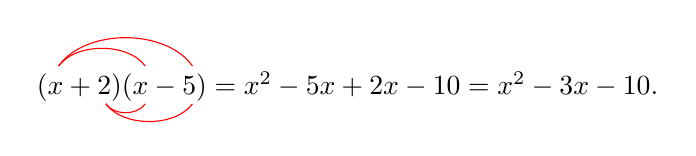
\begin{tikzpicture}
\draw node[right] {$(x+2)(x-5) = x^2-5x+2x-10 = x^2 -3x-10.$};

\pgfmathsetmacro{\klAx}{0.40}
\pgfmathsetmacro{\klBx}{1.00}
\pgfmathsetmacro{\klCx}{1.5}
\pgfmathsetmacro{\klDx}{2.1} % oli 2.8
\pgfmathsetmacro{\klEx}{3.64}
\pgfmathsetmacro{\klLo}{-0.22}
\pgfmathsetmacro{\klHi}{0.26}

\pbezier{\klAx}{\klCx}{\klHi}{0.3}
\pbezier{\klAx}{\klDx}{\klHi}{0.48}

\pbezier{\klBx}{\klCx}{\klLo}{-0.15}
\pbezier{\klBx}{\klDx}{\klLo}{-0.3}
\end{tikzpicture}\newline
\end{esimerkki}

\begin{esimerkki}
Laske binomien $x^2-x$ ja $2x-1$ tulo. \\
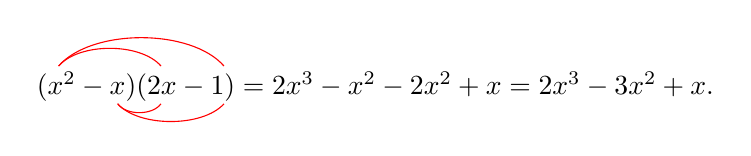
\begin{tikzpicture}
\draw node[right] {$(x^2-x)(2x-1) = 2x^3-x^2-2x^2+x = 2x^3 -3x^2 +x.$};

\pgfmathsetmacro{\klAx}{0.40}
\pgfmathsetmacro{\klBx}{1.15}
\pgfmathsetmacro{\klCx}{1.7}
\pgfmathsetmacro{\klDx}{2.5}
\pgfmathsetmacro{\klEx}{3.64}
\pgfmathsetmacro{\klLo}{-0.22}
\pgfmathsetmacro{\klHi}{0.26}

\pbezier{\klAx}{\klCx}{\klHi}{0.3}
\pbezier{\klAx}{\klDx}{\klHi}{0.48}

\pbezier{\klBx}{\klCx}{\klLo}{-0.15}
\pbezier{\klBx}{\klDx}{\klLo}{-0.3}
\end{tikzpicture}\newline
\end{esimerkki}

\subsubsection*{Yleinen kertolasku}

Osittelulain nojalla kahden polynomin tulo saadaan laskemalla yhteen kaikki
termit, jotka saadaan kertomalla termi ensimmäisestä ja toinen termi toisesta
polynomista.


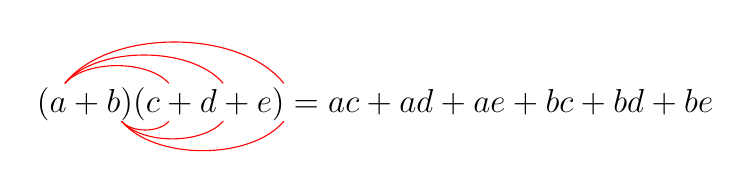
\begin{tikzpicture}
\draw node[right] {\large $(a+b)(c+d+e) = ac+ad+ae+bc+bd+be$};

\pgfmathsetmacro{\klAx}{0.48}
\pgfmathsetmacro{\klBx}{1.20}
\pgfmathsetmacro{\klCx}{1.8}
\pgfmathsetmacro{\klDx}{2.49}
\pgfmathsetmacro{\klEx}{3.26}
\pgfmathsetmacro{\klLo}{-0.22}
\pgfmathsetmacro{\klHi}{0.26}

\pbezier{\klAx}{\klCx}{\klHi}{0.3}
\pbezier{\klAx}{\klDx}{\klHi}{0.48}
\pbezier{\klAx}{\klEx}{\klHi}{0.7}

\pbezier{\klBx}{\klCx}{\klLo}{-0.15}
\pbezier{\klBx}{\klDx}{\klLo}{-0.3}
\pbezier{\klBx}{\klEx}{\klLo}{-0.5}
\end{tikzpicture}

\begin{esimerkki}
Laske polynomien $x-3$ ja $x^2-4x+3$ tulo. \\
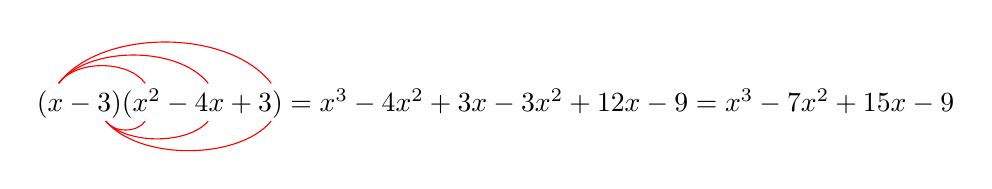
\begin{tikzpicture}
\draw node[right] {$(x-3)(x^2-4x+3) = x^3-4x^2+3x-3x^2+12x-9 = x^3-7x^2+15x-9$};

\pgfmathsetmacro{\klAx}{0.40}
\pgfmathsetmacro{\klBx}{1.00}
\pgfmathsetmacro{\klCx}{1.5}
\pgfmathsetmacro{\klDx}{2.3}
\pgfmathsetmacro{\klEx}{3.1}
\pgfmathsetmacro{\klLo}{-0.22}
\pgfmathsetmacro{\klHi}{0.26}

\pbezier{\klAx}{\klCx}{\klHi}{0.3}
\pbezier{\klAx}{\klDx}{\klHi}{0.48}
\pbezier{\klAx}{\klEx}{\klHi}{0.7}

\pbezier{\klBx}{\klCx}{\klLo}{-0.15}
\pbezier{\klBx}{\klDx}{\klLo}{-0.3}
\pbezier{\klBx}{\klEx}{\klLo}{-0.5}
\end{tikzpicture}\newline
\end{esimerkki}

\begin{esimerkki}
Laske polynomien $x^4-3x^3+3$ ja $x^3-2x^2+1$ tulo. \\
\begin{align*}
&\hspace{0.5cm}(\textcolor{red}{x^4} \textcolor{blue}{-3x^3} +{}\textcolor{green}{3})(x^3-2x^2+1) \\
&= \textcolor{red}{x^4}\cdot x^3 + \textcolor{red}{x^4}\cdot (-2x^2)+\textcolor{red}{x^4}\cdot 1\textcolor{blue}{{}-3x^3}\cdot x^3\textcolor{blue}{{}-3x^3}\cdot(-2x^2)\textcolor{blue}{{}-3x^3}\cdot1 \\
&\hspace{0.5cm}+\textcolor{green}{3}x^3+\textcolor{green}{3}\cdot(-2x^2)+\textcolor{green}{3}\cdot 1 \\
&= x^7-2x^6+x^4-3x^6+6x^5-3x^3+3x^3-6x^2+3 \\
&= x^7-5x^6+6x^5+x^4-6x^2+3
\end{align*}
\end{esimerkki}

\subsection*{Muistikaavat}

\qrlinkki{http://opetus.tv/maa/maa2/muistikaavat/}{
Opetus.tv: \emph{muistikaavat} (8:05, 6:38 ja 9:08)}

Joitakin polynomien kertolaskuja tarvitaan niin usein, että niitä kutsutaan \termi[muistikaavoiksi]{muistikaavat}.

\laatikko{
    \textbf{Muistikaavat}
    \begin{itemize}
        \item $(a+b)^2 = a^2+2ab+b^2$
        \item $(a-b)^2 = a^2-2ab+b^2$
        \item $(a+b)(a-b) = a^2-b^2$
    \end{itemize}
}

Nämä kaavat voidaan todistaa helposti laskemalla.

\paragraph*{Summan neliö}

\begin{align*}
(a+b)^2 &= (a+b)(a+b) &\emph{neliön määritelmä} \\
% &= a(a+b)+b(a+b) &\emph{osittelulaki} \\
&= a^2+ab+ba+b^2 &\emph{osittelulaki} \\
&= a^2+ab+ab+b^2 &\emph{vaihdannaisuus ($ba=ab$)} \\
&= a^2+2ab+b^2
\end{align*}

\paragraph*{Erotuksen neliö}

\begin{align*}
(a-b)^2 &= (a-b)(a-b) &\emph{neliön määritelmä} \\
% &= a(a-b)-b(a-b) &\emph{osittelulaki} \\
&= a^2-ab-ba+b^2 &\emph{osittelulaki} \\
&= a^2-ab-ab+b^2 &\emph{vaihdannaisuus ($ba=ab$)} \\
&= a^2-2ab+b^2
\end{align*}

Edellä todistettuja kahta muistikaavaa kutsutaan yhdessä nimellä binomin neliö. Toisinaan ne kirjoitetaan yhtenä yhtälönä muodossa $(a \pm b)^2=a^2 \pm 2ab+b^2$. % Kaavoissa useasti esiintyviä $\pm$-merkkejä luetaan siten, että ylemmät ja alemmat täsmäävät keskenään. Ylempien merkkien (kaikki $+$:ia) valinta vastaa siis summan neliötä ja alempien merkkien (kaikki $-$:ia) valinta erotuksen neliötä.

\paragraph*{Summan ja erotuksen tulo}

\begin{align*}
(a+b)(a-b) &= a^2-ab+ba-b^2 &\emph{osittelulaki} \\
&= a^2-ab+ab-b^2 &\emph{vaihdannaisuus ($ba=ab$)} \\
&= a^2-b^2
\end{align*}

\begin{esimerkki}
Sievennä $(3x-2y)^2$. \\
\quad\\
Käytetään muistikaavaa $(a-b)^2 = a^2-2ab+b^2$. Nyt $a = 3x$ ja $b = 2y$.
Saadaan
        \[ (3x+2y)^2 = (3x)^2-2\cdot 3x\cdot 2y+(2y)^2 = 9x^2-12xy+4y^2. \]
\end{esimerkki}

\begin{esimerkki}
Laske päässä a) $995^2$ b) $104 \cdot 96$. \\
Käytetään ovelasti muistikaavoja $(a-b)^2 = a^2-2ab+b^2$ ja $(a+b)(a-b) = a^2-b^2$.
\begin{enumerate}[a)]
\item $995^2 = (1000-5)^2 = 1000^2-2\cdot 1000\cdot 5+5^2 = 1000000-10000+25 = 990025 $
\item $104\cdot 96 = (100+4)(100-4) = 100^2 - 4^2 = 10000 - 16 = 9984$.
\end{enumerate}
\end{esimerkki}

\Harjoitustehtavat

\paragraph*{Opi perusteet}

\begin{tehtava}
    Sievennä.
    \begin{enumerate}[a)]
        \item $2(x+3)$
        \item $x(x - 2)$
        \item $3x(1-2x)$
        \item $x^2(x + 5)$
    \end{enumerate}
    \begin{vastaus}
        \begin{enumerate}[a)]
            \item $2x+6$
            \item $x^2 - 2x$
            \item $3x-6x^2$
            \item $x^3 + 5x$
        \end{enumerate}
    \end{vastaus}
\end{tehtava}

\begin{tehtava}
    Sievennä.
    \begin{enumerate}[a)]
        \item $3(x+2y-4)$
        \item $(x+2)(x + 3)$
        \item $(3-x)(2x-1)$
\end{enumerate}
    \begin{vastaus}
        \begin{enumerate}[a)]
            \item $3x+6y-12$
            \item $x^2 +5x+6$
            \item $-2x^2+7x-3$
        \end{enumerate}
    \end{vastaus}
\end{tehtava}

\begin{tehtava}
    Kerro sulut auki muistikaavan avulla.
    \begin{enumerate}[a)]
        \item $(x+y)^2$
        \item $(x-y)^2$
        \item $(x+y)(x-y)$
    \end{enumerate}
    \begin{vastaus}
        \begin{enumerate}[a)]
        \item $x^2 +2xy+y^2$
        \item $x^2 -2xy +y^2$
        \item $x^2-y^2$
        \end{enumerate}
    \end{vastaus}
\end{tehtava}

\begin{tehtava}
    Kerro sulut auki muistikaavan avulla.
    \begin{enumerate}[a)]
        \item $(x+3)^2$
        \item $(y-5)^2$
        \item $(x-4)(x+4)$
        \item $(3x+2)^2$
    \end{enumerate}
    \begin{vastaus}
        \begin{enumerate}[a)]
        \item $x^2 +6x+9$
        \item $y^2 - 10y+25$
        \item $x^2 -16$
        \item $9x^2 +12x +4$
        \end{enumerate}
    \end{vastaus}
\end{tehtava}

\paragraph*{Hallitse kokonaisuus}

\begin{tehtava}
    Sievennä.
    \begin{enumerate}[a)]
        \item $(-2x)(4x - 1)\cdot 3$
        \item $(-x^3)(10x - 2)$
        \item $5(-2x + 1)(-9x) $
        \item $2x(x-3)+1$
    \end{enumerate}
    \begin{vastaus}
        \begin{enumerate}[a)]
            \item $-24x^2 + 6x$
            \item $-10x^4 + 2x^3$
            \item $90x^2 - 45x$
            \item $2x^2-6x+1$
        \end{enumerate}
    \end{vastaus}
\end{tehtava}

\begin{tehtava}
    Sievennä muistikaavojen avulla.
    \begin{enumerate}[a)]
        \item $(5-x)^2$
        \item $(7x + 4)^2$
        \item $(9 - 7x)(9 + 7x)$
        \item $(8x - 8)(8x + 8)$
    \end{enumerate}
    \begin{vastaus}
        \begin{enumerate}[a)]
            \item $x^2 - 10x + 25$
            \item $49x^2 + 56x + 16$
            \item $-49x^2 + 81$
            \item $64x^2 - 64$
        \end{enumerate}
    \end{vastaus}
\end{tehtava}

\begin{tehtava}
    Sievennä.
    \begin{enumerate}[a)]
        \item $(2y+5)(y+7)$
        \item $(x-1)(x+4)x$
    \end{enumerate}
    \begin{vastaus}
        \begin{enumerate}[a)]
            \item $2y^2 + 19y + 35$
            \item $x^3 + 3x^2 - 4x$
        \end{enumerate}
    \end{vastaus}
\end{tehtava}

\begin{tehtava}
    Sievennä.
    \begin{enumerate}[a)]
        \item $(t+v)^2+(t-v)^2$
        \item $(t+v)^2-(t-v)^2$
    \end{enumerate}
    \begin{vastaus}
        \begin{enumerate}[a)]
            \item $(t+v)^2+(t-v)^2 = t^2+2tv+v^2+t^2-2tv+v^2 = 2t^2+2v^2$
            \item $(t+v)^2-(t-v)^2 = t^2+2tv+v^2-t^2+2tv-v^2 = 4tv$
        \end{enumerate}
    \end{vastaus}
\end{tehtava}

\begin{tehtava}
	Sievennä. 
	\begin{enumerate}[a)]
		\item $(x-3)(2x^3-3x+4)$
		\item $(x^2+1)(x^3-2x-4)$
		\item $(x-1)(x^4+x^3+x^2+x+1)$
		\item $(\frac x5-\frac23)(x^2+x+1)$
	\end{enumerate}
	\begin{vastaus}
		\begin{enumerate}[a)]
			\item $2x^4-6x^3-3x^2+13x-12$
			\item $x^5-x^3-4x^2-2x-4$
			\item $x^5-1$
			\item $\frac15x^3-\frac{7}{15}x^2-\frac{7}{15}x-\frac23$
		\end{enumerate}
	\end{vastaus}
\end{tehtava}

\begin{tehtava}
    Sievennä.
    \begin{enumerate}[a)]
            \item $(a+b)^3$
            \item $(a+b)^4$
            \item $(a-b)^3$
        \end{enumerate}
    \begin{vastaus}
        \begin{enumerate}[a)]
            \item $(a+b)^3 = a^3 + 3a^2b + 3ab^2 + b^3$
            \item $(a+b)^4 = a^4 + 4a^3b + 6a^2b^2 + 4ab^3 + b^4$
            \item $(a-b)^3 = a^3 - 3a^2b + 3ab^2 - b^3$
        \end{enumerate}
    \end{vastaus}
\end{tehtava}

\begin{tehtava} %Vaikea!
    Kahden luvun keskiarvo on $7$. Kuinka suuri niiden tulo voi korkeintaan olla?
    \begin{vastaus}
        $49$. Perustelu muistikaavoilla: $(7+a)(7-a)=7^2-a^2 = 49-a^2 \geq 49$
    \end{vastaus}
\end{tehtava}

\paragraph*{Sekalaisia, lajittele}

\begin{tehtava}
    Sievennä lauseke $(x^2+1)(x^3-2x)$. Mikä on polynomin aste?
    \begin{vastaus}
        Lauseke sievenee muotoon $x^5-x^3-2x$. Polynomin aste on $5$.
    \end{vastaus}
\end{tehtava}

\begin{tehtava}
    Määritä sulkuja avaamatta lausekkeen $(x^2+1)(x^3-2x)$
    \begin{enumerate}[a)]
        \item aste
        \item vakiotermi.
    \end{enumerate}
    \begin{vastaus}
        \begin{enumerate}[a)]
            \item Polynomin aste on kunkin tekijän korkeimpien asteiden summa, tässä siis $2+3=5$.
            \item Polynomin vakiotermi on kunkin tekijän vakiotermien tulo, tässä siis $1\cdot 0=0$.
        \end{enumerate}
    \end{vastaus}
\end{tehtava}


\begin{tehtava}
    Sievennä. (Ohje: käytä summakaavoja.)
    \begin{enumerate}[a)]
        \item $63^2+37^2$
        \item $101^2+99^2$
    \end{enumerate}
    \begin{vastaus}
        \begin{enumerate}[a)]
            \item $63^2+37^2 = (50+13)^2+(50-13)^2 = 2\cdot 50^2 + 2\cdot 13^2 = 2\cdot 2500 +2\cdot 169 = 5000 + 338 = 5338$
            \item $101^2+99^2 = (100+1)^2+(100-1)^2 = 2\cdot 100^2 + 2\cdot 1^2 = 2\cdot 10000 + 2\cdot 1 = 20000 + 2 = 20002$
        \end{enumerate}
    \end{vastaus}
\end{tehtava}

\begin{tehtava}
    Sievennä.
    \begin{enumerate}[a)]
        \item $35^2-25^2$
        \item $170^2-50^2$
    \end{enumerate}
    \begin{vastaus}
        \begin{enumerate}[a)]
            \item $35^2-25^2 = (30+5)^2-(30-5)^2 = 4\cdot 30\cdot 5 = 600$
            \item $170^2-30^2 = (100+70)^2+(100-70)^2 = 4\cdot 100\cdot 70 = 28000$
        \end{enumerate}
    \end{vastaus}
\end{tehtava}

\begin{tehtava}
    Olkoon $P(x)=-x^4+2x$ reaalifunktio. Sievennä lausekkeet.
    \begin{enumerate}[a)]
		\item $P(\sqrt{2})$
        \item $P(x)^2$
        \item $P(-x)$
        \item $P(2t)$
    \end{enumerate}
    \begin{vastaus}
        \begin{enumerate}[a)]
            \item $-4 + 2\sqrt{2}$
            \item $x^8 - 4x^5 + 4x^2$
            \item $-x^4-2x$
            \item $-16t^4+4t$
        \end{enumerate}
    \end{vastaus}
\end{tehtava}

\begin{tehtava}
    Olkoot $P(x)=x^2$ ja $Q(x)=x+1$ reaalifunktioita. Sievennä lausekkeet.
    \begin{enumerate}[a)]
        \item $P(x+1)$
        \item $Q(x-1)$
        \item $P(Q(x))$
        \item $Q(P(x))$
    \end{enumerate}
    \begin{vastaus}
        \begin{enumerate}[a)]
            \item $P(x+1) = (x+1)^2 = x^2+2x+1$
            \item $Q(x-1) = (x-1)+1 = x$
            \item $P(Q(x)) = P(x+1) = (x+1)^2 = x^2+2x+1$
            \item $Q(P(x)) = Q(x^2) = x^2+1$
        \end{enumerate}
    \end{vastaus}
\end{tehtava}

	%polynomin kertominen monomilla a(x+b)=ax+ab
	%kahden binomin tulo: (a+b)(c+d)=ac+ad+bc+bd
	%tekijöihin jako, käsite tekijä
	%muistikaavat
		%(a+b)^2=a^2+2ab+b^2
		%(a-b)^2=a^2-2ab+b^2
		%(a-b)(a+b)=a^2-b^2
		%Esimerkki tai harjoitustehtävä: 102*98=(100+2)(100-2)=10000-4
	\section{Tekijöihinjako}

\qrlinkki{http://opetus.tv/maa/maa2/polynomin-jakaminen-tekijoihin/}{Opetus.tv: \emph{polynomin jakaminen tekijöihin} (9:50 ja 5:44)}


%Pitkän matematiikan 1. kurssilla on käsitelty lukujen jakamista tekijöihin.
Esimerkiksi luvun $12$ \termi{tekijä}{tekijät} ovat luvut $1$, $2$, $3$, $4$, $6$ ja $12$. Nämä ovat sellaisia
lukuja, joista saadaan luku $12$ kertomalla ne jollain kokonaisluvulla, tai toisin sanottuna luku $12$ voidaan jakaa
millä tahansa näistä luvuista ilman jakojäännöstä.
%Sanotaan myös, että luvun $12$ \termi{alkutekijä}{alkutekijät} ovat $2$ ja $3$, koska luku $12$ voidaan
%ilmaista niiden tulona ($2\cdot 2\cdot 3 = 2^2\cdot 3 = 12$), mutta näitä tekijöitä ei
%voi enää jakaa pienempiin osatekijöihin. Kokonaisluvun tekijät ovat kokonaislukuja ja alkutekijät alkulukuja.

\begin{esimerkki}
Luku $12$ voidaan kirjoittaa tekijöidensä tulona monella eri tavalla. Esimerkiksi
\begin{align*}
&12 = 2 \cdot 6, \\
&12= 4 \cdot 3 \text{ tai } \\
&12= 2 \cdot 2 \cdot 3.
\end{align*}
\end{esimerkki}

Polynomeja voidaan jakaa vastaavalla tavalla tekijöihin. Polynomien tapauksessa tekijöihinjako tarkoittaa
polynomin esittämistä saman- tai pienempiasteisten polynomien tulona. Aste on aina pienempi, ellei kyse ole pelkästä
vakiokertoimen ottamisesta yhteiseksi tekijäksi.

\begin{esimerkki}
Jaa tekijöihin polynomi $10x^3-20x^2$.
\begin{align*}
& 10x^3-20x^2 \\
=& 10(x^3-2x^2) \ \ \ \ &\emph{otetaan $10$ yhteiseksi tekijäksi} \\
=& 10x^2(x-2) &\emph{otetaan $x^2$ yhteiseksi tekijäksi} \\
\end{align*}
\end{esimerkki}

\begin{esimerkki}
Jaa tekijöihin \quad a) $x^3+x$ \quad b) $3x^2+6x.$

Kun jokaisessa termissä on sama tekijä, se voidaan ottaa yhteiseksi tekijäksi:
\begin{enumerate}[a)]
    \item $x^3+x = x(x^2+1)$
    \item $3x^2+6x = 3x(x+2)$.
\end{enumerate}
\end{esimerkki}

\begin{esimerkki}
Jaa tekijöihin polynomi $5x^3-20x^2+20x$.
\begin{align*}
& 5x^3-20x^2+20x \\
=& 5(x^3-4x^2+4x) \ \ \ \ &\emph{otetaan $5$ yhteiseksi tekijäksi} \\
=& 5x(x^2-4x+4) &\emph{otetaan $x$ yhteiseksi tekijäksi} \\
=& 5x(x^2-2\cdot 2x+2^2) &\emph{sovelletaan muistikaavaa} \\
=& 5x(x-2)^2
\end{align*}
\end{esimerkki}

\begin{esimerkki}
Jaa tekijöihin \quad a) $x^2-4$ \quad b) $x^2+8x+16.$

Jaetaan polynomit tekijöihin hyödyntämällä muistikaavoja
\begin{enumerate}[a)]
    \item $x^2-4 = x^2-2^2 = (x+2)(x-2)$
    \item $x^2+8x+16 = x^2+ 2\cdot 4 \cdot x + 4^2 = (x+4)^2$
\end{enumerate}
\end{esimerkki}

%On suositeltavaa tarkistaa itse, että yllä esitetyt tekijöihinjaot todella toimivat. Polynomien tekijöihinjaon toimivuus
%on helppoa tarkistaa -- täytyy vain laskea väitettyjen tekijöiden tulo ja katsoa, onko se alkuperäinen polynomi. Vaikka
%tarkistus onkin helppoa, tässä vaiheessa ei luultavasti vielä ole selvää, miten tekijöihinjaon voisi saada selville
%-- paitsi toisinaan arvaamalla, mutta tähän kysymykseen vastataan myöhemmin tällä kurssilla.

%Polynomien tekijöihinjako ei ole yksiselitteinen, mutta monesti hyödyllisintä on jakaa polynomi tekijöihin samoin kuin
%esimerkkitapauksissa eli niin, että ensimmäisenä on vakiotermi ja kaikissa muissa tekijäpolynomeissa korkeimman asteen
%termin kerroin on 1.
%
%Esimerkki selkeyttänee asiaa. Polynomi $6x^2+30x+36$ voidaan jakaa tekijöihin vaikkapa seuraavilla tavoilla:
%
%\begin{esimerkki}
%\qquad \\
%\begin{itemize}
%    \item $6(x+2)(x+3)$
%    \item $3(2x+4)(x+3)$
%    \item $3(x+2)(2x+6)$
%    \item $2(3x+6)(x+2)$
%    \item $(6x+12)(x+3)$
%    \item $(\frac12 x+1)(12x+36)$
%\end{itemize}
%\end{esimerkki}
%
%Kaikki nämä tavat ovat ''oikein,'' mutta lähes aina ensimmäinen muoto $6(x+2)(x+3)$ on kätevin.
%
%Toisinaan polynomeille voi löytää tekijöitä soveltamalla joitakin seuraavista keinoista:
%
%\begin{itemize}
%\item Otetaan korkeimman asteen termin kerroin yhteiseksi tekijäksi: \\
%$5x^4+3x^2+x-9 = 5(x^4+\frac{3}{5} x^2+\frac{1}{5} x-\frac{9}{5})$
%\item Otetaan $x$ tai sen potenssi yhteiseksi tekijäksi, jos mahdollista: \\
%$x^5+x^3+3x = x(x^4+x^2+3)$
%$x^7+x^6+5x^4+2x^2 = x^2(x^5+x^4+5x^2+2)$
%\item Sovelletaan muistikaavaa käänteisesti \\
%$x^2-5=x^2-\sqrt{5}^2=(x+\sqrt{5})(x-\sqrt{5})$ \\
%$x^2+8x+16=x^2+2\cdot 4x+4^2=(x+4)^2$ \\
%$x^2+x+\frac14=x^2+2\cdot \frac12 x+(\frac12)^2=(x+\frac12)^2$
%\end{itemize}

Kaikkien polynomien tekijöihinjako ei kuitenkaan näillä menetelmillä onnistu. Myöhemmin tässä kirjassa opitaan, miten toisen asteen polynomin voidaan jakaa tekijöihin nollakohtiensa avulla.

Seuraavassa esimerkissä tekijöihin jako on toteutettu termien ryhmittelyn avulla. Se on joissain tapauksissa näppärä tapa jakaa polynomi tekijöihin, mutta oikean ryhmittelyn keksimiseen ei ole mitään sääntöä.

\begin{esimerkki}
Jaa tekijöihin $x^3+3x^2+x+3$.
\begin{equation*}
x^3+3x^2+x+3=x^2(x+3)+1(x+3)=(x^2+1)(x+3)
\end{equation*}
\end{esimerkki}

\begin{esimerkki}
Jaa tekijöihin $x^{11}+2x^{10}+3x+6$.
\begin{align*}
& x^{11}+2x^{10}+3x+6=x^{10}(x+2)+3(x+2)=(x^{10}+3)(x+2)
\end{align*}
\end{esimerkki}

\begin{tehtavasivu}

\paragraph*{Opi perusteet}

\begin{tehtava}
    Esitä tulona ottamalla yhteinen tekijä.
    \begin{enumerate}[a)]
        \item $2x+6$
        \item $x^2 -4x$
        \item $3x^2 - 6x$
    \end{enumerate}
    \begin{vastaus}
        \begin{enumerate}[a)]
        \item $2(x+3)$
        \item $x(x-4)$
        \item $3x(x-2)$
        \end{enumerate}
    \end{vastaus}
\end{tehtava}

\begin{tehtava}
    Jaa tekijöihin.
    \begin{enumerate}[a)]
        \item $-15^5 +10y$
        \item $x^3y^2 +x^2y^3$
        \item $-4a^3 -2a^2 +2ab$
    \end{enumerate}
    \begin{vastaus}
        \begin{enumerate}[a)]
        \item joko $5(-3x^5 +2y)$ tai $-5(3x^5 -2y)$
        \item $x^2y^2(x+y)$
        \item joko $2a(-2a^2 -a +b)$ tai $-2a(2a^2 +a -b)$
        \end{enumerate}
    \end{vastaus}
\end{tehtava}

\begin{tehtava}
    Jaa tekijöihin.
    \begin{enumerate}[a)]
        \item $x^2+6x+9$
        \item $y^2 - 2y+1$
        \item $x^2 -25$
    \end{enumerate}
    \begin{vastaus}
        \begin{enumerate}[a)]
        \item $(x+3)^2$
        \item $(y-1)^2$
        \item $(x-5)(x+5)$
        \end{enumerate}
    \end{vastaus}
\end{tehtava}

\begin{tehtava}
    Jaa tekijöihin.
    \begin{enumerate}[a)]
        \item $4x^2 +4x +1$
        \item $4x^2 +4x +4$
        \item $9-x^2$
          \end{enumerate}
    \begin{vastaus}
        \begin{enumerate}[a)]
        \item $(2x+1)^2$
        \item $4(x^2 +x +1)$
        \item $(3+x)(3-x)$
        \end{enumerate}
    \end{vastaus}
\end{tehtava}

\begin{tehtava}
    Jaa tekijöihin.
    \begin{enumerate}[a)]
        \item $x^3 +x^2 +x +1$
        \item $a^3 +a^2b +2a +2b$
        \item $4m^5 -2m^3 +2m^2 -1$
    \end{enumerate}
    \begin{vastaus}
        \begin{enumerate}[a)]
        \item $(x^2+1)(x+1)$
        \item $(a^2+2)(a+b)$
        \item $(2m^3 -1)(2m^2 -1)$
        \end{enumerate}
    \end{vastaus}
\end{tehtava}

\paragraph*{Hallitse kokonaisuus}

\begin{tehtava}
    Jaa tekijöihin.
    \begin{enumerate}[a)]
    	\item $x^3 - x$
        \item $x^2 - x + \frac{1}{4} $
        \item $9-x^4$
    \end{enumerate}
    \begin{vastaus}
        \begin{enumerate}[a)]
            \item $x(x-1)^2$
            \item $(x-\frac{1}{2})^2$
            \item $(3+x^2)(3-x^2)$
        \end{enumerate}
    \end{vastaus}
\end{tehtava}

\begin{tehtava}
    Jaa tekijöihin.
    \begin{enumerate}[a)]
    	\item $x^2 -4$
    	\item $x^2 -3$
    	\item $5x^2 -3$
    \end{enumerate}
    \begin{vastaus}
        \begin{enumerate}[a)]
            \item $(x+2)(x-2)$
            \item $(x+\sqrt{3})(x-\sqrt{3})$
            \item $(\sqrt{5}x+\sqrt{3})(\sqrt{5}x-\sqrt{3})$
        \end{enumerate}
    \end{vastaus}
\end{tehtava}

\begin{tehtava}
	Jaa tekijöihin.
	\begin{enumerate}[a)]
		\item $4-x^2$
		\item $16-x^4$
		\item $2-x$
	\end{enumerate}
	\begin{vastaus}
		\begin{enumerate}
			\item $-(x+2)(x-2)$
			\item $-(x^2+4)(x^2-4)$
			\item $-(\sqrt{x}-\sqrt{2})(\sqrt{x}+\sqrt{2})$
		\end{enumerate}
	\end{vastaus}
\end{tehtava}

\paragraph*{Lisää tehtäviä}

\begin{tehtava}
	Jaa tekijöihin. Voit tarvittaessa piirtää kuvaajan
		\begin{enumerate}[a)]
		\item $x-\frac{1}{2}$
		\item \{[ \star ]\} $x^2-x-6$
		\item \{[ \star ]\} $(x-4)^2-9$
	\end{enumerate}
	\begin{vastaus}
		\begin{enumerate}
			\item $\left(\sqrt{x}-\frac{1}{\sqrt{2}}\right)\left(\sqrt{x}+\frac{1}{\sqrt{2}}\right)$
			\item $(x-3)(x+2)$
			\item $(x-1)(x-7)$
		\end{enumerate}
	\end{vastaus}
\end{tehtava}

\end{tehtavasivu}

	\section{Tulon nollasääntö ja tulon merkkisääntö}

\subsection*{Tulon merkkisääntö}

Pitkän matematiikan 1. kurssilla on esitetty seuraava sääntö kahden luvun tulolle:

\laatikko{
    \emph{Tulon merkkisääntö kahdelle tulontekijälle}
    \begin{itemize}
        \item Jos tulon tekijät ovat samanmerkkisiä, tulo on positiivinen.
        \begin{itemize}
	        \item Kahden positiivisen luvun tulo on positiivinen.
	        \item Kahden negatiivisen luvun tulo on positiivinen.
        \end{itemize}
        \item Jos tulon tekijät ovat erimerkkisiä, tulo on negatiivinen.
        \begin{itemize}
	        \item Positiivisen ja negatiivisen luvun tulo on negatiivinen.
        \end{itemize}
    \end{itemize}
}

Useasti käytetty merkkisäännöstä saatava tulos on $x^2 \geq 0$.

%Tulon merkkisääntö yleistyy mille tahansa määrälle tulontekijöitä.

%\laatikko{
%    \emph{Tulon merkkisääntö}
%    \begin{itemize}
%        \item Jos tulossa on parillinen $(0, 2, 4, \ldots)$ määrä negatiivisia tekijöitä, tulo on positiivinen.
%        \begin{itemize}
%	        \item Erityisesti, jos tulossa on vain positiivisia tekijöitä, tulo on positiivinen.
%        \end{itemize}
%        \item Jos tulossa on pariton $(1, 3, 5, \ldots)$ määrä negatiivisia tekijöitä, tulo on negatiivinen.
%    \end{itemize}
%}

Hyödynnämme merkkisääntöä myöhemmin, kun teemme epäyhtälöistä merkkikaavioita.

\subsection*{Tulon nollasääntö}

Tulon merkkisäännöstä seuraa, että positiivisten ja negatiivisten lukujen tulo on aina positiivinen tai negatiivinen, ei koskaan nolla.

Jos siis tulo on $0$, tulon tekijöistä ainakin yhden täytyy olla $0$. Toisaalta $0\cdot x = 0$ kaikilla reaaliluvuilla $x$.
(Todistus tälle on liitteessä \ref{tod:tulonolla}.)

Nämä tiedot yhdistämällä saadaan tulon nollasääntö:

\laatikko{
    \emph{Tulon nollasääntö}
    \begin{itemize}
   	    \item Jos jokin tulon tekijöistä on $0$, tulo on $0$.
   	    \item Jos tulo on $0$, ainakin yksi tulon tekijöistä on $0$.
    \end{itemize}
}

Tulon nollasääntöä on kätevää soveltaa monissa tilanteissa.

\begin{esimerkki} Ratkaistaan yhtälö $(x+5) \cdot x =0 $.
    \begin{align*}
        (x+5)\cdot x &=0 \quad \ppalkki \text{ tulon nollasääntö} \\
        x +5= 0 \text{ tai } x &=0 \\
        x= -5 \text{ tai } x &=0.
    \end{align*}
    Ratkaisuja on siis kaksi, $x= -5$ tai $x= 0$.
\end{esimerkki}

%\begin{esimerkki}
%	\[2(x+5)=0\]
%	Nyt tulon nollasäännön perusteella tiedetään, että $2=0$ tai $x+5=0$.
%	Koska selvästi $2\neq 0$, jää ainoaksi ratkaisuksi $x+5=0$ eli $x=-5$.
%\end{esimerkki}

\begin{esimerkki} Ratkaistaan $y$ yhtälöstä
    \[(x^5+5x+5)\cdot 0\cdot \sqrt{x^3-1} =y\]
    Koska vasemmalla puolella yksi tulon tekijöistä on $0$, tiedämme, että tulo on $0$. Siis $y=0$.
\end{esimerkki}

\begin{esimerkki} Ratkaise yhtälö
    \[xyz=0.\]
Tulon nollasäännön perusteella $x=0$, $y=0$ tai $z=0$. Nollia voi siis
olla 1--3 kappaletta.
\end{esimerkki}

Tulon nollasääntö on yksi tärkeimmistä syistä siihen, miksi polynomien tekijöihinjako on hyödyllistä.

Jos vaikkapa haluamme ratkaista yhtälön $2x^3-14x^2+32x-24=0$ ja satumme tietämään, että $2x^3-14x^2+32x-24=2(x-3)(x-2)^2$,
voimme helposti päätellä, että polynomi saa arvon $0$ jos ja vain jos $x-3=0$ tai $x-2=0$. Yhtälön ainoat ratkaisut ovat siis $x=3$ ja $x=2$.

\begin{esimerkki}
Ratkaise yhtälö $6x^3-36x^2+54x=0$ tulon nollasäännön avulla.
\begin{esimratk}
\begin{align*}
6x^3-36x^2+54x &= 0 \\
6(x^3-6x^2+9x) &= 0 && \ppalkki \text{ otetaan } 6 \text{ yhteiseksi tekijäksi} \\
6x(x^2-6x+9) &= 0 && \ppalkki \text{ otetaan } x \text{ yhteiseksi tekijäksi} \\
6x(x^2-2\cdot 3\cdot x+3^2)  &= 0 \\
6x(x-3)^2 &= 0 & \\
6x(x-3)(x-3) &= 0 && \ppalkki \text{ tulon nollasääntö}\\
6x=0 \textrm{\quad tai}& \quad x-3=0 \\
x=0 \textrm{\quad tai}& \quad x=3 \\
\end{align*}
\end{esimratk}
\begin{esimvast}
$x=0$ tai $x=3$.
\end{esimvast}
\end{esimerkki}

Myöhemmin tässä kirjassa esitetään polynomien jakolause, joka antaa vielä syvällisemmän yhteyden polynomien nollakohtien ja tekijöiden välille.

\Harjoitustehtavat

\begin{tehtava}
    Ratkaise seuraavat yhtälöt käyttämällä tulon nollasääntöä.
    \begin{enumerate}
        \item $x^2(3+x)=0$
        \item $0=x^3(x-5)$
        \item $(x-4)(x^2-4)=0$
    \end{enumerate}
    \begin{vastaus}
        \begin{enumerate}
            \item $x=0$ tai $x=-3$
            \item $x=0$ tai $x=5$
            \item $x=-2$, $x=2$ tai $x=4$
        \end{enumerate}
    \end{vastaus}
\end{tehtava}

\begin{tehtava}
    Ratkaise seuraavat yhtälöt käyttämällä tulon nollasääntöä.
    \begin{enumerate}
        \item $(x^2-1)(x-7)=0$
        \item $(x^2-9)(x^2-16)=0$
        \item $(x-4)=x(x-4)$
    \end{enumerate}
    \begin{vastaus}
        \begin{enumerate}
            \item $x=-1$, $x=1$ tai $x=7$
            \item $x=-4$, $x=-3$, $x=3$ tai $x=4$
            \item $x=1$ tai $x=4$
        \end{enumerate}
    \end{vastaus}
\end{tehtava}

\begin{tehtava}
    Ratkaise seuraavat yhtälöt käyttämällä tulon nollasääntöä.
    \begin{enumerate}
        \item $(\smiley{}+1)\cdot (t+1)=0$
        \item $x(x-5)=0$
        \item $(2w+2)^2=0$
    \end{enumerate}
    \begin{vastaus}
        \begin{enumerate}
            \item $\smiley{}=-1$ tai $t=-1$,\qquad  Symboli $\smiley{}$ esittää jotain lukua, sillä muutoin laskutoimitukset eivät olisi mielekkäitä. Tehtävässä ei myöskään ole selvää, minkä muuttujan suhteen yhtälö pitäisi ratkaista. Siksi on ratkaistu molempien muuttujien suhteen.
            \item $x=0$ tai $x=5$
            \item $w=-1$
        \end{enumerate}
    \end{vastaus}
\end{tehtava}

\begin{tehtava}
    Sievennä seuraava lauseke: $(a-x)\cdot(b-x)\cdot(c-x)\cdot...\cdot(\mathring{a}-x)\cdot(\ddot{a}-x)\cdot(\ddot{o}-x)$.
    \begin{vastaus}
        Tulossa esiintyy tekijänä $(x-x)=0$. Niinpä tulon nollasäännön mukaan
        \begin{align*}
            &(a-x)\cdot(b-x)\cdot(c-x)\cdot...\cdot(x-x)\cdot(y-x)\cdot(z-x)\cdot(\mathring{a}-x)\cdot(\ddot{a}-x)\cdot(\ddot{o}-x) \\
            =&(a-x)\cdot(b-x)\cdot(c-x)\cdot...\cdot 0\cdot(y-x)\cdot(z-x)\cdot(\mathring{a}-x)\cdot(\ddot{a}-x)\cdot(\ddot{o}-x) \\
            =&0
        \end{align*}
    \end{vastaus}
\end{tehtava}

	%tulon nollasääntö
		%tulo on 0 jos ja vain jos ainakin yksi tulon tekijöistä on 0
		%esim. yhtälön x(x-2)=0 ratkaisu
		%korostetaan lyhyesti, että kyseessä on reaalilukujen ominaisuus, joka ei kaikissa muissa joukoissa välttämättä päde
		%liitteeseen voi ajan riittäessä laittaa eksplisiittisen esimerkin tällaisesta joukosta
	%tulon merkkisääntö
		%positiivinen * positiivinen = positiivinen
		%positiivinen * negatiivinen = negatiivinen
		%negatiivinen * negatiivinen = positiivinen
		%sovellus: x^2>=0
	%on hyvä mainita, että säännöt voidaan todistaa
	%todistukset korkeintaan liitteeksi
	\section{Polynomifunktion kuvaaja}
Polynomifunktiota voi
havainnollistaa koordinaatistoon piirretyn kuvaajan avulla:

%\begin{kuvaajapohja}{1.5}{-2}{2}{-3}{3}
%\kuvaaja{-x-1}{$P(x) = -x-1$}{red}
%\kuvaaja{x**2+x}{$Q(x) = x^2+x$}{blue}
%\kuvaaja{x**3-3*x-1}{$R(x) = x^3-3x-1$}{green}
%\end{kuvaajapohja}

\begin{kuvaajapohja}{1.5}{-2}{2}{-3}{3}
%\kuvaaja{-x-1}{$P(x) = -x-1$}{red}
\kuvaaja{x**2+x}{$Q(x) = x^2+x$}{black}
\kuvaaja{x**3-3*x-1}{$R(x) = x^3-3x-1$}{black}
\end{kuvaajapohja}
%
\subsection*{Kuvaajan piirtäminen}

\qrlinkki{http://opetus.tv/maa/maa2/suoran-piirtaminen/}{Opetus.tv: \emph{suoran piirtäminen} (5:47)}

Funktioiden kuvaajia voi piirtää laskimella tai tietokoneella. Kuvaajaa voi myös hahmotella käsin laskemalla funktion arvoja muutamilla muuttujan arvoilla, merkitsemällä pisteet
$xy$-koordinaatistoon ja piirtämällä lopuksi kuvaajaan pisteiden kautta kulkeva viiva.

\begin{esimerkki}
Hahmotellaan polynomifunktion $f(x) = \dfrac{1}{2}x^2 - x - 2$ kuvaaja.
Lasketaan ensin joitakin funktion $f(x) = \dfrac{1}{2}x^2 - x - 2$ arvoja ja piirretään niitä vastaavat pisteet
koordinaatistoon. Lopuksi hahmotellaan kuvaaja, joka kulkee pisteiden kautta.

\begin{tabular}{c c c}
	\begin{tabular}{|c|r @{,} l|}
	\hline $x$ & \multicolumn{2}{c|}{$f(x)$} \\
	\hline
	-3 & 5&5 \\
	-2 & 2&0 \\
	-1 & -0&5 \\
	0 & -2&0 \\
	1 & -2&5 \\
	2 & -2&0 \\
	3 & -0&5 \\
	\hline
	\end{tabular}
	&
	\vcent{\begin{kuvaajapohja}{0.6}{-4}{4}{-3}{6}
	\kuvaajapiste{-3}{5.5}
	\kuvaajapiste{-2}{2}
	\kuvaajapiste{-1}{-0.5}
	\kuvaajapiste{0}{-2}
	\kuvaajapiste{1}{-2.5}
	\kuvaajapiste{2}{-2}
	\kuvaajapiste{3}{-0.5}
	\end{kuvaajapohja}}
	&
	\vcent{\begin{kuvaajapohja}{0.6}{-4}{4}{-3}{6}
	\kuvaajapiste{-3}{5.5}
	\kuvaajapiste{-2}{2}
	\kuvaajapiste{-1}{-0.5}
	\kuvaajapiste{0}{-2}
	\kuvaajapiste{1}{-2.5}
	\kuvaajapiste{2}{-2}
	\kuvaajapiste{3}{-0.5}
	\kuvaaja{0.5*x**2-x-2}{}{black}
	\end{kuvaajapohja}}
\end{tabular}

\end{esimerkki}

\subsection*{Kuvaajan tulkintaa}

%Ensimmäisen asteen polynomin kuvaaja on luonnollisesti aina suora. 
%miten niin luonnollisesti?

Kuvaajan avulla voidaan tehdä johtopäätöksiä funktion ominaisuuksista.
Esimerkiksi funktion arvoja voidaan lukea kuvaajasta.

\begin{esimerkki}
Seuraavassa on esitetty polynomifunktion $P(x)=-3x^2+2x+4$ kuvaaja.

\begin{kuvaajapohja}[\kuvaajaAsetusEiRuudukkoa]{0.7}{-3}{3}{-5}{5}
\kuvaajapiste{2}{-4}
\kuvaajakohtaarvo{2}{-4}{}{}
\kuvaaja{-3*x**2+2*x+4}{$P(x)$}{black}
\end{kuvaajapohja}

Kuvaajasta voi lukea funktion arvoja tai ainakin niiden likiarvoja. Kuvaajan perusteella näyttää siltä, että $P(2)=-4$. Näin todellakin on, sillä $P(1)=-3\cdot 1^2+2\cdot 1+4=1$.
\end{esimerkki}

\begin{esimerkki}
Kuvaajasta ei välttämättä näe tarkkoja arvoja. Seuraavassa on esitetty erään polynomifunktion $P(x)$ kuvaaja. Kuvaajan perusteella näyttäisi siltä, että $P(1)=1$, mutta tarkkaa arvoa kuvaajasta ei voi päätellä.
 
\begin{kuvaajapohja}[\kuvaajaAsetusEiRuudukkoa]{1}{-2}{2}{-2}{2}
\kuvaaja{19./20*x**2+19./20*x-1}{$P(x)$}{black}
\end{kuvaajapohja}
 
Itse asiassa edellinen kuvaaja kuuluu funktiolle $P(x)=\dfrac{19}{20} x^2-\dfrac{19}{20} x-1$. Nyt tiedetään, että funktion $P(x)$ arvo kohdassa $x=1$ on
$$\dfrac{19}{20}\cdot 1^2-\dfrac{19}{20} \cdot 1-1=\dfrac{9}{10}$$
eikä $1$, kuten kuvaajan perusteella voisi luulla. Kuvaajasta ei siis voi lukea tarkkoja tietoja funktiosta.
\end{esimerkki}

Funktion \termi[nollakohta]{nollakohta} on sellainen muuttujan arvo, jolla funktio saa arvon nolla. Esimerkiksi funktiolla $Q(x)=x^2-1$
on nollakohdat $-1$ ja $1$, sillä $Q(-1)=0$ ja $Q(1)=0$.

Funktion kuvaaja antaa tietoa nollakohdista. Niiden kohdalla kuvaaja leikkaa $x$-akselin.

\begin{esimerkki}
Funktion $P(x) = \dfrac{1}{3}x^2-4x+\dfrac{5}{2}$ kuvaajasta nähdään, että funktiolla on ainakin kaksi nollakohtaa. Toinen niistä on lähellä lukua $1$ ja toinen lukua $11$.

\begin{kuvaajapohja}{0.3}{-5}{15}{-10}{5}
\kuvaajapiste{0.66146}{0}
\kuvaajapiste{11.3385}{0}
\kuvaaja{1./3*x**2-4*x+5./2}{$P(x) = \dfrac{1}{3}x^2-4x+\dfrac{5}{2}$}{black}
\end{kuvaajapohja}
\end{esimerkki}

%Nollakohta tarkoittaa sitä annetun polynomin muuttujan arvoa, jolla koko
%polynomi saa arvon nolla. Kuvaajasta sen voi helposti lukea niinä kohtina,
%joissa kuvaaja leikkaa muuttujan koordinaattiakselin. Funktion $P(x)$ ja
%$xy$-koordinaatiston tapauksessa funktion nollakohdat ovat täsmälleen ne
%$x$-koordinaatit, joilla funktion kuvaaja leikkaa $x$-akselin.

%\subsection{Taylorin sarja}
%Eräs mielenkiintoinen ja hyvin tunnettu potenssisarja on Taylorin sarja.
%Se on päättymätön potenssisarja, jolla voidaan approksimoida muiden funktioiden
%arvoja.
%
%Yleisesti Taylorin sarjalla saadaan (rajatta derivoituvan) funktion $f$ arvo
%pisteessä $x_0$:
%
%\begin{align*}
%	f(x_0) = \sum\limits_{n=0}^\infty a_n(x-x_0)^n
%\end{align*}
%
%missä
%
%\begin{align*}
%a_n = \frac{f^n(x_0)}{n!}
%\end{align*}
%
%Koska sarja on äärettömän pitkä, sarjan arvoja edelleen arvioidaan Taylorin
%polynomilla, joka on muotoa
%
%\begin{align*}
%	P_k(x) = \sum\limits_{n=0}^k a_k(x-x_0)^k
%\end{align*}
%
%Polynomin avulla voidaan laskea esimerkiksi likiarvo funktiolle
%$(1-x)^{-1} = \frac{1}{1-x}$ pisteen a ympäristössä, kun $a \neg 1$:
%
%\begin{align*}
%	\frac{1}{1-x} \approx \frac{1}{1-a} + \frac{x-a}{(1-a)^2} +
%\frac{(x-a)^2}{(1-a)^3} + \frac{(x-a)^3}{(1-a)^4} ...
%\end{align*}
%
%\missingfigure{Funktion $(x-1)^-1$ kuvaaja}
%\missingfigure{Funktion $\frac{1}{1-a} + \frac{x-a}{(1-a)^2} +
%\frac{(x-a)^2}{(1-a)^3} +$ kuvaaja}

\Harjoitustehtavat

\begin{tehtava}
    Piirrä polynomien kuvaajat.
    \begin{enumerate}[a)]
        \item $5$
        \item $2x-3$
        \item $x^2+x-2$
        \item $x^3-x+3$
    \end{enumerate}   
    \begin{vastaus}
    	\item \begin{kuvaajapohja}{0.4}{-4}{4}{-1}{7}
				\kuvaaja{5}{}{red}
			  \end{kuvaajapohja}
    	\item \begin{kuvaajapohja}{0.4}{-4}{4}{-5}{3}
				\kuvaaja{2*x-3}{}{red}
			  \end{kuvaajapohja}
		\item \begin{kuvaajapohja}{0.4}{-4}{4}{-3}{5}
				\kuvaaja{x**2+x-2}{}{red}
			  \end{kuvaajapohja}
		\item \begin{kuvaajapohja}{0.4}{-4}{4}{-3}{5}
				\kuvaaja{x**3-x+2}{}{red}
			  \end{kuvaajapohja}
    \end{vastaus}
\end{tehtava}

\begin{tehtava}
    Piirrä polynomien kuvaajat.
    \begin{enumerate}[a)]
        \item $x+4$
        \item $2x-9$
        \item $5x+2$
        \item $6x+1$
    \end{enumerate}
    \begin{vastaus}
        \item \begin{kuvaajapohja}{0.4}{-4}{4}{-1}{7}
				\kuvaaja{x+4}{}{red}
			  \end{kuvaajapohja}
    	\item \begin{kuvaajapohja}{0.4}{-2}{6}{-6}{2}
				\kuvaaja{2*x-9}{}{red}
			  \end{kuvaajapohja}
		\item \begin{kuvaajapohja}{0.4}{-4}{4}{-2}{6}
				\kuvaaja{5*x+2}{}{red}
			  \end{kuvaajapohja}
		\item \begin{kuvaajapohja}{0.4}{-4}{4}{-2}{6}
				\kuvaaja{6*x+1}{}{red}
			  \end{kuvaajapohja}
    \end{vastaus}
\end{tehtava}

\begin{tehtava}
    Piirrä polynomien kuvaajat.
    \begin{enumerate}[a)]
        \item $x^2-1$
        \item $2x^2$
        \item $4x^2+4$
        \item $x^2-6x+3$
    \end{enumerate}
    \begin{vastaus}
        \item \begin{kuvaajapohja}{0.4}{-4}{4}{-2}{6}
				\kuvaaja{x+4}{}{red}
			  \end{kuvaajapohja}
    	\item \begin{kuvaajapohja}{0.4}{-4}{4}{-1}{7}
				\kuvaaja{2*x-9}{}{red}
			  \end{kuvaajapohja}
		\item \begin{kuvaajapohja}{0.4}{-4}{4}{-1}{11}
				\kuvaaja{5*x+2}{}{red}
			  \end{kuvaajapohja}
		\item \begin{kuvaajapohja}{0.4}{-1}{7}{-7}{5}
				\kuvaaja{6*x+1}{}{red}
			  \end{kuvaajapohja}
    \end{vastaus}
\end{tehtava}

\begin{tehtava}
    Piirrä polynomien kuvaajat.
    \begin{enumerate}[a)]
        \item $5x^2$
        \item $3x^2+4$
        \item $2x^2-10$
        \item $x^2-x-1$
    \end{enumerate}
    \begin{vastaus}
        \item \begin{kuvaajapohja}{0.4}{-4}{4}{-1}{7}
				\kuvaaja{5*x**2}{}{red}
			  \end{kuvaajapohja}
    	\item \begin{kuvaajapohja}{0.4}{-4}{4}{-1}{11}
				\kuvaaja{3*x**2+4}{}{red}
			  \end{kuvaajapohja}
		\item \begin{kuvaajapohja}{0.4}{-4}{4}{-11}{1}
				\kuvaaja{2*x**2-10}{}{red}
			  \end{kuvaajapohja}
		\item \begin{kuvaajapohja}{0.4}{-3}{5}{-2}{6}
				\kuvaaja{x**2-x-1}{}{red}
			  \end{kuvaajapohja}
    \end{vastaus}
\end{tehtava}

\begin{tehtava}
	Monia funktioita voidaan esittää likimääräisesti polynomeina (ns.
Taylorin polynomi). Esimerkiksi

	\begin{tabular}{lcll}
	$\frac{1}{1+x^2}$ &$\approx$ & $1-x^2+x^4-x^6+x^8-x^{10}$, & kun
$-1<x<1$ \\
	$\sqrt{1+x}$ & $\approx $ & $ 1+\frac{x}{2}
	-\frac{x^2}{8}+\frac{x^3}{16}-\frac{5x^4}{128}$, & kun $-1<x<1$
	\end{tabular}

	Piirrä alkuperäinen funktio ja polynomi samaan kuvaajaan tietokoneella
tai graafisella laskimella. Kokeile, kuinka polynomin viimeisten termien pois
jättäminen vaikuttaa tarkkuuteen. Mitä havaitset? (Termejä voi laskea lisääkin,
mutta siihen ei puututa tässä.)

	\begin{vastaus}
		Mitä enemmän termejä, sitä parempi vastaavuus.
	\end{vastaus}
\end{tehtava}

	%tarkoituksena varmistaa, että opiskelijat:
		%muistavat koordinaatiston idean
		%osaavat hahmotella funktion kuvaajan laskemalla sen arvoja
		%osaavat lukea funktion arvoja kuvaajasta sekä
		%oppivat käsitteen nollakohta
	%esimerkkeinä polynomeja
	%mitään yleistä teoriaa polynomien kuvaajista ei tarvita, mainittakoon että ensimmäisen asteen funktion kuvaaja on suora

\chapter{Ensimmäinen aste}
	%% encoding: utf-8
\section{Kertausta: Ensimmäisen asteen yhtälö}

Yhtälöistä yksinkertaisin on ensimmäisen asteen yhtälö. Käydään se lyhyesti
läpi kertauksen vuoksi.

Ensimmäisen asteen yhtälössä ratkaistavana on vain mahdollisesti vakiolla
kerrottu muuttuja. Yhtälön ratkaisemiseksi riittää käyttää neljää
aritmeettista peruslaskutoimitusta. Aluksi yhtälön molempia puolia
lisätään tai vähennetään jollain luvulla, jolloin
vasemmalle puolelle saadaan jäämään pelkkä muuttuja
vakiolla kerrottuna.
Sen jälkeen jaetaan yhtälön molemmat puolet muuttujan kertoimella, jolloin
yhtälön ratkaisu jää oikealle puolelle.

% fixme tyylikorjausta, termiä juuri ei vielä esitellä

Yleisesti ensimmäisen asteen yhtälö on muotoa

\begin{align*}
    ax + b = 0.
\end{align*}

Mikä vain 1. asteen yhtälö on muokattavissa tähän yleiseen
muotoon siirtämällä kaikki termit vasemmalle puolelle ja
sieventämällä.

\subsubsection*{Esimerkkejä}

\begin{esimerkki}
Ratkaise yhtälö $4x + 5 = 2 + 2x$.

\textbf{Ratkaisu}
\begin{align*}
    4x + 5 &= 2 + 2x && \ppalkki -2x \\
    2x + 5 &= 2      && \ppalkki -5 \\
        2x &= -3     && \ppalkki :2 \\
         x &= -\frac{3}{2}
 \end{align*}
\end{esimerkki}

\begin{esimerkki}
Ratkaise yhtälö $3x - 6 = 0$.

\textbf{Ratkaisu}
  \begin{align*}
    3x - 6 &= 0 && \ppalkki +6 \\
        3x &= 6 && \ppalkki :3 \\
         x &= \frac{6}{3} \\
           &= 2
  \end{align*}
\end{esimerkki}

Yleisen yhtälön $ax + b = 0$ ratkaisu on siis

\begin{align*}
  x = -\frac{b}{a}.
\end{align*}

Erityisesti kannattaa huomata, että kaikkia 1. asteen yhtälöitä ei tarvitse
saattaa yleiseen muotoon. Esimerkiksi jos vakiotermit ovat valmiiksi
oikealla puolella, yhtälön ratkaisemiseksi riittää luonnollisesti jakaa
molemmat puolet muuttujan kertoimella.

\Harjoitustehtavat

\paragraph*{Opi perusteet}

\begin{tehtava}
    Ratkaise yhtälöt.
    \begin{enumerate}[(a)]
        \item $x + 5 = 47$
        \item $2x = 64$
        \item $3x - 5 = 16$
    \end{enumerate}
    \begin{vastaus}
        \begin{enumerate}[(a)]
            \item $x = 42$
            \item $x = 32$
            \item $x = 7$
        \end{enumerate}
    \end{vastaus}
\end{tehtava}

\begin{tehtava}
    Ratkaise yhtälöt.
    \begin{enumerate}[(a)]
        \item $x + 8 = 2x - 1$
        \item $2x + 4 = 60$
        \item $3x - 5 = -x + 11$
    \end{enumerate}
    \begin{vastaus}
        \begin{enumerate}[(a)]
            \item $x = 9$
            \item $x = 28$
            \item $x = 4$
        \end{enumerate}
    \end{vastaus}
\end{tehtava}

%ei ole yhtälötehtävä, mutta mallinnusharjoituksena ok? 
\begin{tehtava}
    Muodosta tilannetta kuvaavat lausekkeet.
    \begin{enumerate}[(a)]
        \item Kuinka paljon maksaa hilavitkuttimen vuokraus $x$:ksi tunniksi, kun vuokra on 42 \euro /tunti. Vuokraajan tulee myös ottaa pakollinen 25 euron laitteistovakuutus.
        \item Kuinka monta euroa saa $x$:llä dollarilla, kun 1~EUR vastaa 1,23~USD:a, ja halutaan vaihtaa dollareita euroiksi. Valuutanvaihtaja veloittaa lisäksi palvelumaksun 0,50 euroa.
    \end{enumerate}
    \begin{vastaus}
        \begin{enumerate}[(a)]
            \item $42x + 25$
            \item $\frac{1}{1{,}23}x + 0{,}5$
        \end{enumerate}
    \end{vastaus}
\end{tehtava}



\paragraph*{Hallitse kokonaisuus}

\begin{tehtava}
    Ratkaise yhtälöt.
    \begin{enumerate}[(a)]
        \item $3(x+7)=7x$
        \item $2(3x-1)=-7x $
        \item $3-2x-(4-x)=2 $
    \end{enumerate}
    \begin{vastaus}
        \begin{enumerate}[(a)]
            \item $x = \frac{7}{6} =1\frac{1}{6} $
            \item $x = \frac{2}{13}$
            \item $x = -3$
        \end{enumerate}
    \end{vastaus}
\end{tehtava}

\begin{tehtava}
    Ratkaise yhtälöt.
    \begin{enumerate}[(a)]
        \item $-2\cdot\frac{x-5}{3}-\frac{5}{7}(1-x)=5x+3$
        \item $\frac{4x-5}{3}-\frac{3}{2}(x-8)=-\frac{x+5}{6}$
        \item $3(x-3)+x=4x-9$
    \end{enumerate}
    \begin{vastaus}
        \begin{enumerate}[(a)]
            \item $x = -\frac{1}{13}$
            \item ei ratkaisuja
            \item yhtälö on toteutuu kaikilla reaaliluvuilla
        \end{enumerate}
    \end{vastaus}
\end{tehtava}

%vaatii Pythagoraan lauseen, jota ei vielä ole käsitelty lukiossa.
\begin{tehtava}
    Tässä tehtävässä pitäisi muistaa peruskoulussa käsitelty Pythagoraan lause.
    Suorakulmaisen kolmion sivujen pituuden kateettien pituudet ovat $x+1$ ja $4$. Hypotenuusan pituus $x+3$. Mikä $x$ on?
    \begin{vastaus}
		$x=2$
    \end{vastaus}
\end{tehtava}

%hankala
\begin{tehtava}
    Määritä sekunnin tarkkuudella se ajanhetki, kun kellotaulun minuutti- ja tuntiviisarit ovat päällekkäin ensimmäisen kerran klo 12.00:n jälkeen.
    \begin{vastaus}
		$13.05.27$
    \end{vastaus}
\end{tehtava}

	%KERTAUSTA lyhyesti
	%tarkoituksena, että tämän voi jättää väliin, jos osaa jo
	%nimitys juuri
	\section{Epäyhtälöistä yleisesti}
Epäyhtälöllä tarkoitetaan ilmausta, jossa esitetään kahden lausekkeen arvon välinen suuruusjärjestys. Suuruusjärjestyksien esittämiseen käytetään seuraavia merkintöjä:

\begin{center}
\begin{tabular}{l|l}
\emph{Merkintä} & \emph{Merkitys} \\
\hline
$a<b$ &  $a$ on pienempi kuin $b$ \\
$a>b$ & $a$ on suurempi kuin $b$ \\
$a \leq b$ & $a$ on pienempi tai yhtäsuuri kuin $b$ \\
$a \geq b$ & $a$ on suurempi tai yhtäsuuri kuin $b$ \\
\end{tabular}
\end{center}

Sama epäyhtälö voidaan kirjoittaa kahdella tavalla: $a < b$ tarkoittaa samaa kuin $b > a$, ja $a \leq b$ tarkoittaa samaa kuin $b \geq a$. Epäyhtälö $a < b$ pätee täsmälleen silloin, kun epäyhtälö $a \geq b$ ei päde.

Epäyhtälön totuusarvo voi riippua epäyhtälön puolilla esiintyvien muuttujien arvoista. Tämän perusteella epäyhtälöt voidaan jakaa kolmeen tyyppiin:
\begin{itemize}
\item \emph{Aina tosi} -- pätee kaikilla muuttujien arvoilla. Esimerkiksi epäyhtälöt $5 < 6$ tai $x + 1 \leq x + 3$ pätevät riippumatta muuttujien arvoista.
\item \emph{Ehdollisesti tosi} -- pätee vain joillain muuttujien arvoilla. Esimerkiksi epäyhtälö $x < 5$ pätee, kun $x = 4$, mutta ei päde, kun $x = 7$.
\item \emph{Aina epätosi} -- ei päde millään muuttujien arvoilla. Esimerkiksi epäyhtälöt $3 < 1$ ja $x < x$ eivät päde koskaan.
\end{itemize}

\subsection*{Epäyhtälöiden muokkaaminen}
Vastaavasti kuten yhtälöiden ratkaisemisessa, epäyhtälön ratkaisemisessa selvitetään ne muuttujien arvot, joilla epäyhtälö on tosi.

Kuten yhtälöitä, myös epäyhtälöitä voidaan ratkaista muokkaamalla niitä sellaisilla operaatioilla, joilla muokattu epäyhtälö on yhtäpitävä alkuperäisen kanssa.

Kahden luvun kasvattaminen saman verran siirtää lukuja lukusuoralla, mutta säilyttää niiden keskinäisen järjestyksen:

\begin{lukusuora}{-1}{10}{12}
	\lukusuoranuolialas{2}{6}
	\lukusuoranuolialas{3}{7}

	\lukusuorapiste{2}{$2$}
	\lukusuorapiste{3}{$3$}
	\lukusuorapystyviiva{0}{$0$}
\lukusuorauusi
	\lukusuorapiste{6}{$2\!+\!4$}
	\lukusuorapiste{7}{$3\!+\!4$}
	\lukusuorapystyviiva{0}{$0$}
\end{lukusuora}

Tämän perusteella epäyhtälö, joka saadaan lisäämällä epäyhtälön molemmille puolille sama lauseke, on yhtäpitävä alkuperäisen epäyhtälön kanssa.

\begin{esimerkki}
Luvun lisääminen epäyhtälöön.
  \begin{align*}
     2 &< 3 && \ppalkki +4\\
   2+4 &< 3+4  \\
     6 &< 7 && tosi
  \end{align*}
\end{esimerkki}

Myös lukujen kertominen samalla positiivisella kertoimella säilyttää niiden keskinäisen järjestyksen. Jos kerroin on pienempi kuin yksi, luvut lähenevät toisiaan:

\begin{lukusuora}{-1}{10}{12}
	\lukusuoranuolialas{2}{1}
	\lukusuoranuolialas{4}{2}

	\lukusuorapiste{2}{$2$}
	\lukusuorapiste{4}{$4$}
	\lukusuorapystyviiva{0}{$0$}
\lukusuorauusi
	\lukusuorapiste{1}{$2 \cdot \frac{1}{2}$}
	\lukusuorapiste{2}{$4 \cdot \frac{1}{2}$}
	\lukusuorapystyviiva{0}{$0$}
\end{lukusuora}

Jos kerroin on suurempi kuin yksi, luvut etääntyvät toisistaan:

\begin{lukusuora}{-1}{10}{12}
	\lukusuoranuolialas{2}{4}
	\lukusuoranuolialas{4}{8}

	\lukusuorapiste{2}{$2$}
	\lukusuorapiste{4}{$4$}
	\lukusuorapystyviiva{0}{$0$}
\lukusuorauusi
	\lukusuorapiste{4}{$2\cdot 2$}
	\lukusuorapiste{8}{$4\cdot 2$}
	\lukusuorapystyviiva{0}{$0$}
\end{lukusuora}

Luvulla jakaminen on sama asia kuin jakajan käänteisluvulla kertominen, joten positiivisella luvulla jakaminen säilyttää järjestyksen kertolaskun tavoin. Näin ollen alkuperäisen epäyhtälön kanssa yhtäpitävä epäyhtälö saadaan kertomalla tai jakamalla molemmat puolet positiivisella luvulla.

\begin{esimerkki}
Epäyhtälön kertominen lukua yksi pienemmällä positiivisella luvulla.
\begin{align*}
     2 &< 4 && \ppalkki \cdot \frac{1}{2} \\
   2\cdot\frac{1}{2} &< 4\cdot\frac{1}{2}  \\
     1 &< 2 && tosi
\end{align*}
\end{esimerkki}

\begin{esimerkki}
Epäyhtälön kertominen lukua yksi suuremmalla luvulla.
\begin{align*}
     2 &< 4 && \ppalkki \cdot 2 \\
   2\cdot 2 &< 4\cdot 2  \\
     4 &< 8 && tosi
\end{align*}
\end{esimerkki}

Sen sijaan negatiivisella luvulla kertominen ei säilytä suuruusjärjestystä. Esimerkiksi kun lukuja 2 ja 5 kerrotaan luvulla $-1$, niiden suuruusjärjestys kääntyy:

\begin{lukusuora}{-6}{6}{12}
	\lukusuoranuolialas{2}{-2}
	\lukusuoranuolialas{5}{-5}

	\lukusuorapiste{2}{$2$}
	\lukusuorapiste{5}{$5$}
	\lukusuorapystyviiva{0}{$0$}
\lukusuorauusi
	\lukusuorapiste{-2}{$2 \cdot (-1)$}
	\lukusuorapiste{-5}{$5 \cdot (-1)$}
	\lukusuorapystyviiva{0}{$0$}
\end{lukusuora}

Jos epäyhtälöä kerrotaan tai jaetaan negatiivisella luvulla, epäyhtälömerkin suunta täytyy kääntää, jotta saataisiin yhtäpitävä epäyhtälö.
%: esimerkissä $2 < 5$ muuttuu muotoon $-2 > -5$.

\begin{esimerkki}
Epäyhtälön kertominen negatiivisella luvulla.
\begin{align*}
     2 &< 5 && \ppalkki \cdot (-1) \\
   2\cdot (-1) &< 4\cdot (-1)  \\
     -2 &> -5 && tosi
\end{align*}
\end{esimerkki}

\laatikko{Epäyhtälöstä saadaan yhtäpitävä epäyhtälö
\begin{itemize}
\item lisäämällä molemmille puolille sama lauseke,
\item kertomalla tai jakamalla molemmat puolet samalla positiivisella luvulla tai
\item kertomalla tai jakamalla molemmat puolet samalla negatiivisella luvulla ja kääntämällä epäyhtälömerkin suunta.
\end{itemize}
}

Kuten yhtälöiden tapauksessa, epäyhtälön kertominen puolittain nollalla ei tuota yhtäpitävää epäyhtälöä, sillä esimerkiksi epäyhtälöstä $a \leq b$ tulee $0 \leq 0$, joka on aina tosi, ja epäyhtälöstä $a < b$ tulee $0 < 0$, joka on aina epätosi.

\begin{esimerkki}
Muokataan epäyhtälöä $-2x+4<6$ käyttämällä esitettyjä operaatioita.
\begin{align*}
-2x+4&<6 && \ppalkki -4 \\
-2x&<2 && \ppalkki :(-2) \\
x&>-1
\end{align*}
Tehdyt operaatiot tuottavat yhtäpitäviä epäyhtälöitä, joten epäyhtälö $-2x+4<6$ on yhtäpitävä epäyhtälön $x>-1$ kanssa. Voidaan päätellä, että lukua $-1$ suuremmat luvut ovat täsmälleen epäyhtälön ratkaisut.
\end{esimerkki}

\subsection*{Reaalilukuvälit}

Ratkaistaessa yhtälöitä ratkaisuksi saadaan yleensä pieni joukko lukuja. Epäyhtälöiden tapauksessa on tyypillistä, että ratkaisu on \termi[väli]{väli}, eli kaikki kahden luvun väliset luvut.

Reaalilukuvälejä merkitään usein laittamalla välin ala- ja ylärajat hakasulkujen sisään. Mikäli ala- tai yläraja ei kuulu väliin, vastaava hakasulku käännetään. Esimerkiksi $[a, b[$ tarkoittaa lukuja $x$ jotka toteuttavat kaksoisepäyhtälön $a \leq x < b$. Väliä kutsutaan \termi[suljetuksi väliksi]{suljettu väli}, mikäli ala- ja yläraja kuuluu väliin, ja \termi[avoimeksi väliksi]{avoin väli}, mikäli ala- ja yläraja eivät kuulu väliin. Jos vain toinen raja kuuluu väliin, väli on \termi[puoliavoin]{puoliavoin väli}.

Väli voidaan piirtää lukusuoralle kahden luvun välisenä janana. Päätepisteet merkitään täytetyllä ympyrällä, mikäli luku kuuluu väliin, ja muuten tyhjällä ympyrällä. Esimerkiksi väli $[a, b[$ piirretään seuraavasti:

\begin{lukusuora}{0}{10}{6}
	\lukusuoravalisa{2}{8}{$a$}{$b$}
\end{lukusuora}

Jos halutaan, että väli ei ole alhaalta tai ylhäältä rajoitettu, merkitään rajaksi $-\infty$ tai $\infty$. Koska ääretön ei ole luku eikä näin ollen kuulu väliin, on sitä vastaava hakasulku käännettävä, ja siten esimerkiksi väli $]{-\infty}, a[$ on avoin. 

Seuraavaan taulukkoon on koottu reaalilukuvälien olennainen käsitteistö ja merkinnät.

\begin{tabular}{|c|p{2.0cm}|p{2.1cm}|c|}
\hline
Välin nimitys & Epäyhtälö\-merkintä & Joukko-opillinen merkintä & Esitys lukusuoralla \\
\hline
Avoin väli & $-3<x<5$ & $x \in {]-3, 5[}$ & \begin{lukusuora}{-6}{10}{4}\lukusuorapystyviiva{0}{$0$}\lukusuoravaliaa{-3}{5}{$-3$}{$5$}\end{lukusuora}\\
\hline
Puoliavoin väli & $-3<x \leq 5$ & $x \in {]-3, 5]}$ & \begin{lukusuora}{-6}{10}{4}\lukusuorapystyviiva{0}{$0$}\lukusuoravalias{-3}{5}{$-3$}{$5$}\end{lukusuora}\\
\hline
Puoliavoin väli & $-3\leq x < 5$ & $x \in {[-3, 5[}$ & \begin{lukusuora}{-6}{10}{4}\lukusuorapystyviiva{0}{$0$}\lukusuoravalisa{-3}{5}{$-3$}{$5$}\end{lukusuora}\\
\hline
Suljettu väli & $-3\leq x \leq 5$ & $x \in {[-3, 5]}$ & \begin{lukusuora}{-6}{10}{4}\lukusuorapystyviiva{0}{$0$}\lukusuoravaliss{-3}{5}{$-3$}{$5$}\end{lukusuora}\\
\hline
Puoliavoin väli & $-3\leq x$ & $x \in {[-3, \infty[}$ & \begin{lukusuora}{-6}{10}{4}\lukusuorapystyviiva{0}{$0$}\lukusuoravalisa{-3}{}{$-3$}{}\end{lukusuora}\\
\hline
Avoin väli & $-3<x$ & $x \in {]-3, \infty[}$ & \begin{lukusuora}{-6}{10}{4}\lukusuorapystyviiva{0}{$0$}\lukusuoravaliaa{-3}{}{$-3$}{}\end{lukusuora}\\
\hline
Puoliavoin väli & $x \leq 5$ & $x \in {]{-\infty}, 5]}$ & \begin{lukusuora}{-6}{10}{4}\lukusuorapystyviiva{0}{$0$}\lukusuoravalias{}{5}{}{$5$}\end{lukusuora}\\
\hline
Avoin väli & $x < 5$ & $x \in {]{-\infty}, 5[}$ & \begin{lukusuora}{-6}{10}{4}\lukusuorapystyviiva{0}{$0$}\lukusuoravaliaa{}{5}{}{$5$}\end{lukusuora}\\
\hline
\end{tabular}

 \begin{esimerkki}
 
 a) Epäyhtälö $2<x<10$ vaatii, että $x$ saa arvoja kahden ja kymmenen väliltä, mutta se ei koskaan saa täsmälleen näitä reuna-arvoja. Kyseessä on avoin väli kahdesta kymmeneen, $]2,10[$. Annetulle epäyhtälölle yhtäpitävä ilmaisu on $x \in ]2,10[$. \\
 b) Epäyhtälö $0\leq y \leq 2$ rajaa muuttujan $y$ välille suljetulle välille $[0,2]$. Väli on suljettu, koska $y$ voi myös saada täsmälleen arvot $0$ ja $2$. \\
 c) Joskus kirjallisuudessa näkee äärettömyyssymbolin käyttöä myös kaksoisepäyhtälöissä, esimerkiksi $3<x<\infty $, mutta ilmaistaan yleisemmin muodossa $x \in ]3,\infty[$. Kyseessä on avoin väli. \\
 d) Epäyhtälöt $-100<k\leq 0$ ja $u\leq 90$ ovat puoliavoimia välejä, koska ne rajaavat muuttujan yhtäsuuruuden avulla vain toiselta puolelta. \\
 e) Kaksoisepäyhtälö $\frac{1}{5}\geq x>-\sqrt{3}$ tarkoittaa samaa kuin kaksoisepäyhtälö $-\sqrt{3}<x\leq \frac{1}{5}$. Kaksoisepäyhtälö vaatii, että muuttujalle $x$ pätee erikseen sekä epäyhtälö $-\sqrt{3}<x$ että $x\leq \frac{1}{5}$.
 \end{esimerkki}

\section{Ensimmäisen asteen epäyhtälö}

\qrlinkki{http://opetus.tv/maa/maa2/ensimmaisen-asteen-epayhtalo/}{Opetus.tv: \emph{ensimmäisen asteen epäyhtälö} (14:55 ja 8:21)}

Harjoittelemme nyt erityisesti 1. asteen epäyhtälöiden ratkaisemista -- toisen asteen ja sitä korkeampien polynomiepäyhtälöiden ratkaisemista käsitellään toisen asteen yhtälön käsittelyn jälkeen.

Samoin kuin yhtälöiden kohdalla, epäyhtälö pyritään muuttamaan niin yksinkertaiseen muotoon kuin mahdollista, jotta yksinkertaisesta tilanteesta nähdään välittömästi, mitkä luvut kuuluvat ratkaisuun ja mitkä eivät. Tuntemattomat pyritään yhdistämään, ja epäyhtälöä muokataan niin, että tuntematon saadaan yksin omalle puolelleen yhtälöä.


\begin{esimerkki}
Ratkaistaan epäyhtälö $2x+1 < 0$.
\begin{align*}
2x+1 &< 0 && \ppalkki -1 \\
2x &< -1 && \ppalkki :2 \\
x &< -\frac{1}{2}
\end{align*}

Epäyhtälön ratkaisu voidaan esittää myös muodossa $x \in ]-\infty, -\frac{1}{2}[$.

Ratkaisua voidaan perustella myös graafisesti tutkimalla lausekkeeseen $2x+1$ liittyvää kuvaajaa:

\begin{kuvaajapohja}{1}{-2}{2}{-2}{2}
	\kuvaaja{2*x+1}{$f(x)=2x+1$}{red}
\end{kuvaajapohja}

Alkuperäinen epäyhtälö $2x+1<0$ vaatii, että lausekkeen $2x+1$ arvo on negatiivinen. Yhtälön ratkaisu on mahdollista nähdä katsomalla kuvasta, millä kaikilla $x$:n arvoilla funktion $2x+1$ kuvaaja laskee vaaka-akselin alapuolelle. Tällöin funktio, siis toisaalta lauseke $2x+1$, saa negatiivisia arvoja.

\end{esimerkki}

\begin{esimerkki}Selvitetään, millä $w$:n arvoilla pätee
$-8w-(8-w) \geq \frac12 w+5$?

\begin{align*}
-8w-(8-w) &\geq \frac12 w+5 \\
-8w-8+w &\geq \frac12 w+5 \\
-7w-8 &\geq \frac12 w+5  \ \ \ \ \ && \ppalkki -\frac12 w \\
-7\frac12 w-8 &\geq 5  \ \ \ \ \ && \ppalkki +8 \\
-7\frac12 w &\geq 13  \ \ \ \ \ && \ppalkki :(-7\frac12) \\
w &\leq 13:(-7\frac12) \\
w &\leq 13:(-\frac{15}{2}) \\
w &\leq -13\cdot \frac{2}{15} \\
w &\leq -\frac{26}{15} \\
w &\leq -1\frac{11}{15}
\end{align*}

Vastaus: $w \leq -1\frac{11}{15}$
\end{esimerkki}

Ensimmäisen asteen polynomiepäyhtälö ratkaistaan siis aivan kuten vastaava yhtälö, mutta negatiivisella luvulla jaettaessa tai kerrottaessa epäyhtälömerkki kääntyy toisin päin.

\begin{esimerkki}
Ratkaistaan kaksoisepäyhtälö $1\leq q+7<-5q+4$.

Tässä on itse asiassa kaksi epäyhtälöä $1\leq q+7$ ja $q+7<-5q+4$. Haluamme siis löytää ne $q$:n arvot, joilla molemmat epäyhtälöt pätevät.
\begin{align*}
1&\leq q+7 \ \ \ \ \ && \ppalkki -7 \\
-6&\leq q
\end{align*}
Vastaavasti toiselle yhtälölle:
\begin{align*}
q+7&<-5q+4  \ \ \ \ \ && \ppalkki +5q \\
6q+7&<4 && \ppalkki -7 \\
6q&<-3 && \ppalkki :6 \\
q&< -\frac12 \\
\end{align*}

Nämä yhdistämällä saadaan $-6\leq q$ ja $q< -\frac12$ eli $-6\leq q < -\frac12$ eli $q\in [-6, -\frac12[$.

\begin{tabular}{cc}
\begin{lukusuora}{-8}{2}{6} \lukusuoravalisa{-6}{}{$-6$}{} \lukusuorapystyviiva{0}{$0$} \end{lukusuora} & $-6\leq q$ \\
\begin{lukusuora}{-8}{2}{6} \lukusuoravaliaa{}{-0.5}{}{$-\frac12$} \lukusuorapystyviiva{0}{$0$} \end{lukusuora} & $q< -\frac12$ \\
\begin{lukusuora}{-8}{2}{6} \lukusuoravalisa{-6}{-0.5}{$-6$}{$-\frac12$} \lukusuorapystyviiva{0}{$0$} \end{lukusuora} & $-6\leq q < -\frac12$ \\
\end{tabular}
\end{esimerkki}

\Harjoitustehtavat

\begin{tehtava}
    Esitä joukko-opillisilla merkinnöillä ja lukusuoralla.
    \begin{enumerate}[a)]
        \item $-9<x \leq 7$
        \item $5\leq c$
        \item $5\leq s \leq 7\frac{1}{2}$
        \item $5\geq x>1$
        \item $a<b$
    \end{enumerate}
    \begin{vastaus}
        \begin{enumerate}[a)]
            \item $x \in ]-9,7]$
            \item $c \in [5,\infty]$
            \item $s \in [5,7\frac{1}{2}]$
            \item $x \in ]1,5]$
            \item $a \in ]-\infty,b[$ \quad tai \quad $b \in ]a, \infty[$
        \end{enumerate}
    \end{vastaus}
\end{tehtava}

\begin{tehtava}
    Ratkaise seuraavat yhtälöt tai epäyhtälöt.
    \begin{enumerate}[a)]
        \item $-2r+6=0$
        \item $-2r+6\leq 0$
        \item $5y-2<y+6$
        \item $8(x+2)\geq -5(5-x)+3$
        \item $\frac{x+3}{2}+\frac{-2x+1}{3}>\frac{x-9}{4}$
    \end{enumerate}
    \begin{vastaus}
        \begin{enumerate}[a)]
            \item $r=3$
            \item $r\geq 3$
            \item $y<2$
            \item $x=-12\frac{2}{3}$
            \item $x<9\frac{4}{5}$
        \end{enumerate}
    \end{vastaus}
\end{tehtava}

\begin{tehtava}
    Ratkaise seuraavat epäyhtälöt.
    \begin{enumerate}[a)]
        \item $3x+6<4x$
        \item $3x-6<2x+57$
        \item $5y-2<12$
        \item $3\leq y+9$
        \item $z-5\geq-888$
    \end{enumerate}
    \begin{vastaus}
        \begin{enumerate}[a)]
            \item $x>6$
            \item $x<63$
            \item $y<2,8$
            \item $y\geq -6$
            \item $z\leq 883$
        \end{enumerate}
    \end{vastaus}
\end{tehtava}

\begin{tehtava}
    Ratkaise seuraavat epäyhtälöt.
    \begin{enumerate}[a)]
        \item $3x+6<2x\leq 9-x$
        \item $3x+6<2x\leq 1+3x$
    \end{enumerate}
    \begin{vastaus}
        \begin{enumerate}[a)]
            \item $x<-6$
            \item ei ratkaisua
        \end{enumerate}
    \end{vastaus}
\end{tehtava}


\begin{tehtava}
	Millä $x$:n arvoilla luvut $2x - 5$, $-x$ ja $x + 4$ ovat erisuuria ja $2x - 5$ on luvuista
	\begin{enumerate}[a)]
		\item suurin
		\item toiseksi suurin
		\item pienin?
	\end{enumerate}
	\begin{vastaus}
		\begin{enumerate}[a)]
			\item $x > 9$
			\item $\frac{5}{3} < x < 9$
			\item $x < \frac{5}{3}$
		\end{enumerate}
	\end{vastaus}
\end{tehtava}

\begin{tehtava}
Lukion päättötodistuksessa aineen arvosana määräytyy aineen pakollisten ja syventävien kurssien keskiarvosta pyöristettynä kokonaisluvuksi tavallisten 
sääntöjen mukaan. Opiskelija haluaa filosofian päättöarvosanakseen 7 tai paremman. Opiskelija aikoo osallistua kolmelle filosofian kurssille. Kahden 
kurssin jälkeen hänen arvosanojensa keskiarvo on 6. Mikä arvosana on opiskelijan vähintään saatava kolmannesta kurssista? Kurssit arvioidaan asteikolla 
4--10.
\begin{vastaus}
%Muodostettava epäyhtälö on muotoa $\frac{2\cdot 6+x}{3}\geq 6.5$, josta ratkaisuna saadaan $x\geq7.5$.
Vähintään arvosana 8.
\end{vastaus}
\end{tehtava}

\begin{tehtava}
	Tietyn auton käyttövoimavero on 450 \euro /vuosi, ja keskimääräinen kulutus on 5 litraa dieselöljyä / 100~km. Saman valmistajan vastaava bensiinikäyttöinen auto kuluttaa 8 litraa / 100~km. Diesel maksaa 1,55 \euro /litra, ja bensiini maksaa 1,65 \euro /litra. Kun vain annetut tiedot huomioidaan, niin kuinka paljon esimerkin dieselajoneuvolla tulee vähintään ajaa vuodessa, jotta se on edullisempi? Dieselauton mahdollista kalliimpaa ostohintaa ei huomioida.
    \begin{vastaus}
        8257 km
    \end{vastaus}
\end{tehtava}

	%yleistä järjestyksestä ja epäyhtälöistä, ratkaisujoukko on reaalilukuväli
	%ensimmäisen asteen epäyhtälö
		%merkin kääntyminen negatiivisella luvulla kerrottaessa perustellaan tulon merkkisäännöllä: jos x>b, x-b>0
		%siis lausekkeella a(x-b) on sama merkki kuin luvulla a

\chapter{Toinen aste}
	\section{Toisen asteen polynomifunktio}

\qrlinkki{http://opetus.tv/maa/maa2/toisen-asteen-polynomifunktio/}{Opetus.tv: \emph{toisen asteen polynomifunktio} (7:59)}

Toisen asteen polynomifunktio on muotoa
\begin{align*}
ax^2+bx+c,
\end{align*}
missä vakiot $b$ ja $c$ voivat olla mitä tahansa reaalilukuja $(b, \ c \in \mathbb{R})$ ja $a$ voi olla mikä tahansa reaaliluku, paitsi luku nolla $(a \in \mathbb{R}, \ a \neq 0)$.

Toisen asteen polynomifunktion kuvaajaa nimitetään \termi[paraabeliksi]{paraabeli}. Jos toisen asteen polynomifunktiossa $a < 0$ sanomme sen kuvaajaa
alaspäin aukeavaksi paraabeliksi ja vastaavasti, kun $a > 0$, kuvaajaa nimitetään ylöspäin aukeavaksi paraabeliksi.

% FIXME: kuvat alaspäin ja ylöspäin aukeavista paraabeleista

	\section{Toisen asteen yhtälö}

\qrlinkki{http://opetus.tv/maa/maa2/toisen-asteen-yhtalo/}{Opetus.tv: \emph{toisen asteen yhtälö} (9:02, 11:09 ja 9:30)}

\begin{esimerkki}
Selvitetään, milloin funktio $f(x)=x^2+2x+1$ leikkaa x-akselin.

Funktion kuvaaja leikkaa x-akselin, kun $f(x)=0$. Tätä muuttujan $x$ arvoa kutsutaan funktion $f$ \textbf{nollakohdaksi}. Piirretään funktion $f$ kuvaaja ja etsitään ne kohdat, joissa funktio leikkaa x-akselin. %insert kuvaaja.pic
%funktio käsite on tuttu, joten itse esittelisin tämän asian näin -Lauri

\begin{kuvaajapohja}{1.5}{-2.5}{0.5}{-0.5}{3}
\kuvaaja{x**2+2*x+1}{$f(x)=x^2+2x+1$}{red}
\end{kuvaajapohja}
\end{esimerkki}

Kuvaajasta havaitaan, että funktion $f$ nollakohta on $x \approx -1$. Tätä funktion nollikohtien ratkaisumenetelmää kutsutaan graafiseksi ratkaisemiseksi.
Graafinen ratkaisu on aina likimääräinen eli arvio oikeasta ratkaisusta.

Määritettäessä toisen asteen polynomifunktion nollakohtia päädytään \textbf{toisen asteen yhtälöön}, joka on aina saatettavissa yleiseen muotoon
\begin{align*}
ax^2+bx+c=0
\end{align*}
\laatikko{Toisen asteen yhtälöllä on reaalilukuratkaisuja joko 0, 1 tai 2 kappaletta.}

Seuraavassa kuvat eri tapauksista:

\begin{tabular}{c c}

\begin{tabular}{c}
	2 ratkaisua, a positiivinen\\
	\begin{lukusuora}{-1}{1}{4}
	\lukusuoraisobbox
	\lukusuoraparaabeli{-0.5}{0.5}{-1}
	\end{lukusuora}
\end{tabular}

&

\begin{tabular}{c}
	2 ratkaisua, a negatiivinen\\
	\begin{lukusuora}{-1}{1}{4}
	\lukusuoraisobbox
	\lukusuoraparaabeli{-0.5}{0.5}{1}
	\end{lukusuora}
\end{tabular}

\\ \qquad & \qquad \\

\begin{tabular}{c}
	1 ratkaisu, a positiivinen\\
	\begin{lukusuora}{-2}{2}{4}
	\lukusuoraisobbox
	\lukusuorakuvaaja{x**2}
	\end{lukusuora}
\end{tabular}

&

\begin{tabular}{c}
	1 ratkaisu, a negatiivinen\\
	\begin{lukusuora}{-2}{2}{4}
	\lukusuoraisobbox
	\lukusuorakuvaaja{-x**2}
	\end{lukusuora}
\end{tabular}

\\ \qquad & \qquad \\

\begin{tabular}{c}
	ei ratkaisuja, a positiivinen\\
	\begin{lukusuora}{-2}{2}{4}
	\lukusuoraisobbox
	\lukusuorakuvaaja{x**2+0.3}
	\end{lukusuora}
\end{tabular}

&

\begin{tabular}{c}
	ei ratkaisuja, a negatiivinen\\
	\begin{lukusuora}{-2}{2}{4}
	\lukusuoraisobbox
	\lukusuorakuvaaja{-x**2-0.3}
	\end{lukusuora}
\end{tabular}

\\ \qquad & \qquad \\

\end{tabular}
% fixme {termi-komento ei toimi vaillinaisen ekvationin kohdalla}

Graafisen ratkaisemisen lisäksi toisen asteen yhtälö voidaan ratkaista
myös algebrallisesti, mihin tutustumme seuraavaksi.
%Seuraavaksi tutustumme toisen asteen yhtälön algebralliseen ratkaisemiseen.

\subsection*{Vaillinaiset yhtälöt}
Jos toisen asteen yhtälöstä $ax^2+bx+c=0$ puuttuu joko termi $bx$ tai $c$, 
kyseessä on niin sanottu \emph{vaillinainen toisen asteen yhtälö}. Se on muotoa
\[ax^2+c=0 \quad \text{ tai } \quad ax^2+bx=0.\]
Vaillinaisten yhtälöiden ratkaiseminen on paljon yleistä tapausta yksinkertaisempaa.

\subsubsection*{Toisen asteen yhtälö $ax^2+c=0$}
Muotoa $ax^2+c = 0$ oleva toisen asteen yhtälö saadaan helposti ratkaistua neliöjuuren avulla.

\begin{esimerkki}
Ratkaistaan yhtälö $5x^2-45=0$:
\begin{align*}
5x^2-45 &= 0 &&\ppalkki + 45 \\
5x^2 &= 45 &&\ppalkki : 5 \\
x^2 &= 9 &&\text{ratkaistaan käyttäen neliöjuurta ($9 \geq 0$)} \\
x &= \pm \sqrt{9} = \pm 3.
\end{align*}
\end{esimerkki}

\begin{esimerkki}
Ratkaistaan yhtälö $13x^2-42=-3$:
\begin{align*}
13x^2-42 &= -3 &&\ppalkki + 42 \\
13x^2 &= 39 &&\ppalkki : 13 \\
x^2 &= 3 &&\text{ratkaistaan käyttäen neliöjuurta ($3 \geq 0$)} \\
x &= \pm \sqrt{3}.
\end{align*}
\end{esimerkki}

\begin{esimerkki}
Ratkaistaan yhtälö $x^2+4=3$:
\begin{align*}
x^2+4 &= 3 &&\ppalkki - 4 \\
x^2 &= -1
\end{align*}
Koska $x^2 \geq 0$ kaikilla $x$, yhtälöllä ei ole ratkaisua.
\end{esimerkki}

\subsubsection*{Toisen asteen yhtälö $ax^2+bx=0$}
Jos yhtälöstä $ax^2+bx+c=0$ puuttuu vakiotermi $c$, yhtälö saa muodon 
$$ax^2+bx=0.$$ Tällainen yhtälö ratkeaa jakamalla tekijöihin ja käyttämällä tulon nollasääntöä:
\begin{align*}
ax^2+bx&=0 \ \ \ \ \ &&\ppalkki\text{otetaan yhteinen tekijä} \\
x(ax+b)&=0 \ \ \ \ \ &&\ppalkki\text{tulon nollasääntö} \\
x&=0 \text{ tai } ax+b=0 \\
x&=0 \text{ tai } ax=-b \\
x&=0 \text{ tai } x=-\frac{b}{a}.
\end{align*}
\begin{esimerkki}
Ratkaise yhtälö $x^2-11x=0$.
\begin{align*}
x^2-11x&=0 \ \ \ \ \  &&\ppalkki\text{otetaan yhteinen tekijä } x\\
x(x-11)&=0 \ \ \ \ \ &&\ppalkki\text{tulon nollasääntö} \\
x&=0 \text{ tai } x-11=0 \\
x&=0 \text{ tai } x=11
\end{align*}
\end{esimerkki}

\begin{esimerkki}
Ratkaise yhtälö $55x^2+8x=0$.
\begin{align*}
55x^2+8x&=0 \ \ \ \ \ &&\ppalkki\text{otetaan yhteinen tekijä} \\
x(55x+8)&=0 \ \ \ \ \ &&\ppalkki\text{tulon nollasääntö} \\
x&=0 \text{ tai } 55x+8=0 \\
x&=0 \text{ tai } 55x=-8 \\
x&=0 \text{ tai } x=-\frac{8}{55}
\end{align*}
\end{esimerkki}

\subsection*{Neliöksi täydentäminen}
Toisen asteen yhtälöä $ax^2+bx+c=0$, jossa $a,b,c \neq 0$, kutsutaan
täydelliseksi toisen asteen yhtälöksi. Tällaiset yhtälöt voidaan palauttaa
vaillinaisiksi toisen asteen yhtälöiksi muistikaavojen avulla.
Tarkastellaan vaikkapa yhtälöä
\[x^2+2x-3=0.\]
Yhtälön vasen puoli on melkein sama kuin binomin $x+1$ neliö, sillä $(x+1)^2=x^2+2x+1$.
Vain vakiotermissä on eroa. Korjataan asia ja ratkaistaan yhtälö:

\begin{align*}
x^2+2x-3 & = 0  &&\ppalkki +4 \\
x^2+2x+1 & = 4  &&\ppalkki \text{ muistikaava: } (x+1)^2=x^2+2x+1. \\
(x+1)^2 & = 4 \\
x+1 & = \pm 2 \\
x & = \pm 2 - 1 \\
x & = 1 \text{ tai } x= -3. 
\end{align*}

Miksi edellä osattiin ajatella juuri oikeaa muistikaavaa $(x+1)^2=x^2+2x+1$?
Syynä on se, että yhtälön vasemmalla
puolella olevan polynomin alkuosaa $x^2+2x$ ei saada minkään muun
binomin neliöstä. Neliöksi täydentäminen vaatii siis muistikaavojen hyvää
hallintaa.

Kaikki toisen asteen yhtälöt voidaan ratkaista neliöksi täydentämällä. (Yleensä tosin käytetään \emph{toisen asteen yhtälön ratkaisukaavaa}, joka esitellään seuraavassa luvussa. Ratkaisukaava perustellaan neliöksi täydentämällä, minkä vuoksi neliöksi täydentäminen opetellaan ensin.)

\begin{esimerkki} Ratkaise yhtälö $x^2+4x-16 = 0$. 

Kirjoitetaan yhtälö muotoon $x^2+2\cdot 2x-16 = 0$ ja verrataan kahta ensimmäistä termiä
muistikaavaan, jotta nähdään, minkä binomin neliöksi lauseke voidaan muokata.
\begin{align*}
&x^2+2\cdot 2\cdot x  &&= (\quad + \quad)^2\\
&a^2 +2\cdot a\cdot b +b^2 &&= (a+b)^2
\end{align*}
Lausekkeita vertaamalla nähdään vastaavuus $a = x$, $b = 2$. Neliöstä puuttuva
termi $b^2$ on siis $2^2=4$. Täydennetään nyt neliöksi:
\begin{align*}
x^2+4x-16 &= 0 \\
x^2+4x &= 16 && \\
x^2+4x+4 &= 20 && \ppalkki \text{muistikaava: $ x^2+4x+4= (x+2)^2$} \\
(x+2)^2 &= 20 \\
x+2 &= \pm \sqrt{20} \\
x &= -2 \pm \sqrt{20} && \ppalkki \text{sievennetään vastaus} \\
x &= -2 \pm 2\sqrt{5}.
\end{align*}
\end{esimerkki}

\begin{esimerkki}
Ratkaistaan yhtälö $4x^2-4x-5=0$.

Toisen ja ensimmäisen asteen termit saadaan neliöstä
$(2x-1)^2=4x^2-4x+1$. Rakennetaan se yhtälön vasemmalle puolelle:
\begin{align*}
4x^2-4x-5 &= 0 \\
4x^2-4x+1 &= 6 &&\text{muistikaava: $  4x^2-4x+1 = (2x-1)^2$} \\
(2x-1)^2 &= 6 \\
2x-1 &= \pm \sqrt{6} \\
2x &= 1 \pm \sqrt{6} \\
x &= \frac{1 \pm \sqrt{6}}{2}.
\end{align*}
\end{esimerkki}

% \textbf{Esimerkki 5.} \\
% Ratkaistaan yhtälö $x^2+4x-16=0$.
% \begin{align*}
% x^2+4x-16&=0 \ \ \ \ \ &&\ppalkki +20 \\
% x^2+4x+4&=20 \ \ \ \ \ &&\ppalkki a^2+2ab+b^2=(a+b)^2 \\
% (x+2)^2&=20 \ \ \ \ \ &&\ppalkki \sqrt[]{} \\
% x+2 &= \pm \sqrt[]{20} \\
% x&=-2 \pm \sqrt[]{20} \\
% x&=-2 \pm 2 \sqrt[]{5} \\
% \end{align*}
% \textbf{Esimerkki 6.} \\
% Ratkaise yhtälö $16x^2-64x+2=0$. \\
% \textbf{Ratkaisu}
% \begin{align*}
% 16x^2-16x+2&=0 \ \ \ \ \ &&\ppalkki +2 \\
% 16x^2-16x+4&=2 \ \ \ \ \ &&\ppalkki a^2-2ab+b^2=(a-b)^2 \\
% (4x+2)^2&=2 \ \ \ \ \ &&\ppalkki \sqrt[]{} \\
% 4x+2&=\pm \sqrt[]{2} \\
% 4x&=-2 \pm \sqrt[]{2} \\
% x&=-\frac{1}{2} \pm \frac{\sqrt[]{2}}{4} \\
% x&=-\frac{1}{2} \pm \frac{\sqrt[]{2}}{ 2\sqrt[]{2}\sqrt[]{2}} \\
% x&=-\frac{1}{2} \pm \frac{1}{2 \sqrt[]{2}} \\
% \end{align*}
%
% Ratkaisutapaa, jossa toisen asteen yhtälö täydennetään lisäämällä tai vähentämällä termejä binomin neliöksi, kutsutaan neliöksi täydentämiseksi.
%
% Toisen asteen yhtälö voidaan aina ratkaista neliöön täydentämällä. Yleensä toisen asteen yhtälöt kuitenkin ratkaistaan käyttämällä suoraa kaavaa.
%
% Seuraavassa kappaleessa johdamme toisen asteen yhtälön ratkaisukaavan neliöksi täydentämistä käyttäen.

\Harjoitustehtavat

\paragraph*{Opi perusteet}

\begin{tehtava}
    Ratkaise yhtälöt.
    \begin{enumerate}[a)]
        \item $x^2 = 16$
        \item $x^2 = - 16$
        \item $x^2 - 13 = 0$
        \item $3x^2 - 12 = 0$

    \end{enumerate}
    \begin{vastaus}
        \begin{enumerate}[a)]
            \item $x=\pm 4$
            \item Ei ratkaisuja. 
            \item $x = \pm \sqrt{13}$.
            \item $x=\pm 2$ 
        \end{enumerate}
    \end{vastaus}
\end{tehtava}

\begin{tehtava}
    Ratkaise yhtälöt.
    \begin{enumerate}[a)]
        \item $x(x-3)= 0$
        \item $x^2 + 4x = 0$
        \item $7x^2-3x = 0$
    \end{enumerate}
    \begin{vastaus}
        \begin{enumerate}[a)]
            \item $x=0$ tai $x=3$
            \item $x =0$ tai $x=-4$.
            \item $x=0$ tai $x=\frac{3}{7}$     
        \end{enumerate}
    \end{vastaus}
\end{tehtava}

\begin{tehtava}
    Kirjoita neliöksi tunnistamalla muistikaava
    \begin{enumerate}[a)]
        \item $x^2 +2x +1 =$
        \item $x^2 +6x +9 = $
        \item $x^2 -4x -4 = $
    \end{enumerate}
    \begin{vastaus}
        \begin{enumerate}[a)]
            \item $(x+1)^2$
            \item $(x+3)^2$.
            \item $(x-2)^2$     
        \end{enumerate}
    \end{vastaus}
\end{tehtava}

\begin{tehtava}
    Ratkaise yhtälö täydentämällä neliöksi
    \begin{enumerate}[a)]
        \item $x^2 -2x +1 = 4$
        \item $x^2 +4x = 5 $
        \item $x^2 -3x + 10 = 0 $
    \end{enumerate}
    \begin{vastaus}
        \begin{enumerate}[a)]
            \item $x = 3$ tai $x= -1$. Neliöksi täydennettynä $(x+1)^2=4$
            \item $x = -5$ tai $x = 1$. Neliöksi täydennettynä $(x+2)^2=9$
            \item Ei ratkaisua. Neliöksi täydennettynä $(x-3)^2=-1$   
        \end{enumerate}
    \end{vastaus}
\end{tehtava}

\paragraph*{Hallitse kokonaisuus}

\begin{tehtava}
    Ratkaise seuraavat yhtälöt.
    \begin{enumerate}[a)]
        \item $x^2 - 100 = 0$
        \item $x^2 + 100 = 0$
        \item $x^2 - 10 = 0$
        \item $x^2 + 10 = 0$
        \item $-x^2 - 25 = 0$
        \item $-x^2 + 25 = 0$
        \item $2x^2 - 98 = 0$
        \item $2x^2 + 98 = 0$
    \end{enumerate}
    \begin{vastaus}
        \begin{enumerate}[a)]
            \item $x=\pm10$
            \item Ei ratkaisuja.
            \item $x=\pm\sqrt{10}$
            \item Ei ratkaisuja.
            \item Ei ratkaisuja.
            \item $x=\pm5$
            \item $x=\pm7$
            \item Ei ratkaisuja.
        \end{enumerate}
    \end{vastaus}
\end{tehtava}

\begin{tehtava}
    Ratkaise seuraavat yhtälöt.
    \begin{enumerate}[a)]
        \item $x^2 - 72x = 0$
        \item $x^2 + 72x = 0$
        \item $x^2 - 56x = 0$
        \item $x^2 + 56x = 0$
        \item $-x^2 - 13x = 0$
        \item $-x^2 + 13x = 0$
        \item $2x^2 - 43x = 0$
        \item $2x^2 + 43x = 0$
    \end{enumerate}
    \begin{vastaus}
        \begin{enumerate}[a)]
            \item $x=0$ tai $x=72$
            \item $x=-72$ tai $x=0$
            \item $x=0$ tai $x=56$
            \item $x=-56$ tai $x=0$
            \item $x=-13$ tai $x=0$
            \item $x=0$ tai $x=13$
            \item $x=0$ tai $x=21,5$
            \item $x=-21,5$ tai $x=0$
        \end{enumerate}
    \end{vastaus}
\end{tehtava}

\begin{tehtava}
    Ratkaise seuraavat yhtälöt.
    \begin{enumerate}[a)]
        \item $x^2 - 36 = 0$
        \item $x^2 - 85x = 0$
        \item $x^2 + 11x = -6x$
        \item $x^2 + 10x = -4x^2$
    \end{enumerate}
    \begin{vastaus}
        \begin{enumerate}[a)]
            \item $x=\pm6$
            \item $x=0$ tai $x=85$
            \item $x=0$ tai $x=-17$
            \item $x=0$ tai $x=-2$
        \end{enumerate}
    \end{vastaus}
\end{tehtava}


\begin{tehtava}
    Ratkaise seuraavat yhtälöt.
    \begin{enumerate}[a)]
        \item $x^2 - 9 = 0$
        \item $2x^2 + 8 = 0$
        \item $-x^2 + 11 = -5$
        \item $3 - x^2 = -1 + 3x^2$
    \end{enumerate}
    \begin{vastaus}
        \begin{enumerate}[a)]
            \item $x=\pm3$
            \item Ei ratkaisuja.
            \item $x=\pm4$
            \item $x=\pm1$
        \end{enumerate}
    \end{vastaus}
\end{tehtava}

\begin{tehtava}
    Ratkaise seuraavat yhtälöt.
    \begin{enumerate}[a)]
        \item $x^2 - 3x = 0$
        \item $10x + 2x^2 = 0$
        \item $-3x^2 + 8x = -2x$
        \item $2x^2 - x^3 = 0$
    \end{enumerate}
    \begin{vastaus}
        \begin{enumerate}[a)]
            \item $x=0$ tai $x=3$
            \item $x=0$ tai $x=-5$
            \item $x=0$ tai $x=8$
            \item $x=0$ tai $x=2$
        \end{enumerate}
    \end{vastaus}
\end{tehtava}

\begin{tehtava}
    Ratkaise seuraavat yhtälöt.
    \begin{enumerate}[a)]
        \item $x^2+3x+2=0$
        \item $2x^2+5x-12=0$
        \item $3x^2-7x-20=0$
        \item $x^2+3x-5=0$
        \item $x^2+5x-24=0$
    \end{enumerate}
    \begin{vastaus}
        \begin{enumerate}[a)]
            \item $x=-2$ tai $x=-1$
            \item $x=3/2$ tai $x=-4$
            \item $x=4$ tai $x=-5/3$
            \item $x=\frac{3\pm\sqrt{29}}{2}$
            \item $x=3$ tai $x=-8$
        \end{enumerate}
    \end{vastaus}
\end{tehtava}

\begin{tehtava}
    Ratkaise seuraavat yhtälöt.
    \begin{enumerate}[a)]
        \item $x^2+3x-5=4x+8$
        \item $8x^2-5x+1=-36$
        \item $-3x^2-4x+2=-5x^2+3$
        \item $-3x^2+4x+13=-5x^2+10x+9$
    \end{enumerate}
    \begin{vastaus}
        \begin{enumerate}[a)]
            \item $\frac{1\pm\sqrt{53}}{2}$
            \item Ei ratkaisua reaalilukujen joukossa.
            \item $1\pm\frac{\sqrt{6}}{2}$
            \item $x=1$ tai $x=2$
        \end{enumerate}
    \end{vastaus}
\end{tehtava}

\begin{tehtava}
    Elokuvassa \emph{Dredd} pudotetaan ihmisiä kuolemaan noin $1$ kilometrin korkeudesta. Ennen pudotusta heille annetaan huumausainetta, joka hidastaa aikakäsityksen $1$ prosenttiin normaalista. Vapaassa pudotuksessa pudottu matka ajanhetkellä $t$ on $\frac{1}{2} gt^2$, jossa $g$ on putoamiskiihtyvyytenä tunnettu vakio, jolle voimme tässä hyvin käyttää arviota $g \approx 10\frac{\text{m}}{\text{s}^2}$.
    \begin{enumerate}[a)]
    \item Olettaen, että huumausaineen vaikutus kestää koko putoamisen ajan, kuinka pitkältä aika pudotuksesta kuolemaan \textbf{uhrista} tuntuu? (Oleta annetut arvot tarkoiksi ja muodosta relevantti toisen asteen yhtälö.)
    \item Mikä menee fataalisti pieleen, jos a)-kohdan laskee suoraan kuvatulla tavalla?
    \end{enumerate}
    \begin{vastaus}
        \begin{enumerate}[a)]
            \item Vastaukseksi saadaan $1414 \, \text{s} = 23 \, \text{min} \, 34 \, \text{s}$. Käytännössä hyvä vastaustarkkuus voisi olla esimerkiksi $25 \, \text{min}$.
            \item Tehtävä ei huomioi ilmanvastusta. Ihminen saavuttaa korkeimmillaan rajanopeuden $v_{raja} \approx 55\frac{\text{m}}{\text{s}}$. Tehtävän mallissa putoavan ihmisen nopeus nousee $v_{max} \approx 141\frac{\text{m}}{\text{s}}$ asti. Todellisuudessa putoaminen siis kestää vieläkin kauemmin.
        \end{enumerate}
    \end{vastaus}
\end{tehtava}

	%toisen asteen yhtälö on muotoa ax^2+bx+c=0
	%vaillinaiset yhtälöt
		%yhtälöt muotoa ax^2+c=0 ja ax^2+bx=0
	%neliöksi täydentäminen
		%tämän voi opettaja halutessaan jättää käsittelemättä
		%idea siitä, että minkä tahansa toisen asteen yhtälön voi ratkaista täydentämällä neliöksi
	\section{Toisen asteen yhtälön ratkaisukaava}

\qrlinkki{http://opetus.tv/maa/maa2/toisen-asteen-yhtalon-ratkaisukaava/}{Opetus.tv: \emph{toisen asteen ratkaisukaava} (9:03, 11:06 ja 10:09)}

Edellisessä kappaleessa opittiin, että toisen asteen yhtälö voidaan aina ratkaista täydentämällä se neliöksi.
Neliöksi täydentämistä käytetään kuitenkin harvoin, sillä saman ajatuksen voi ilmaista valmiina kaavana.
Johdetaan seuraavassa toisen asteen yhtälön ratkaisukaava. \\ \\

Lähdetään liikkeelle täydellisestä toisen asteen yhtälöstä $ax^2+bx+c=0$.
\begin{align*}
ax^2+bx+c&=0 &&\textnormal{\footnotesize{kerrotaan molemmat puolet termillä}} \ 4a \\
4a \cdot ax^2+4a \cdot bx + 4a \cdot c&=0 \\
4a^2x^2+4abx+4ac&=0 &&\textnormal{\footnotesize{vähennetään puolittain termi}} \ 4ac  \\
4a^2x^2+4abx&=-4ac
\end{align*}
Täydennetään vasen puoli binomin neliöksi.
\begin{align*}
4a^2x^2+4abx&=-4ac &&\textnormal{\footnotesize{lisätään puolittain termi}} \ b^2 \\
4a^2x^2+4abx+b^2&=b^2-4ac &&\textnormal{\footnotesize{neliö:}} \ 4a^2x^2+4abx+b^2=(2ax+b)^2 \\
(2ax+b)^2&=b^2-4ac &&\textnormal{\footnotesize{otetaan puolittain neliöjuuri, jos}} \ b^2 \geq 4ac \\
2ax+b&= \pm \sqrt[]{b^2-4ac} &&\textnormal{\footnotesize{vähennetään puolittain termi}} \ b \\
2ax&=-b \pm \sqrt[]{b^2-4ac} &&\textnormal{\footnotesize{jaetaan puolittain termillä}} \ 2a \neq 0 \\
x&= \frac{-b \pm \sqrt[]{b^2-4ac}}{2a}
\end{align*}
Toisen asteen yhtälön ratkaisukaava on siis \[x= \frac{-b \pm \sqrt[]{b^2-4ac}}{2a}\] oletuksella, että $b^2 \geq 4ac$. Oletus tarvitaan, koska negatiivisille luvuille ei ole reaaliluvuilla määriteltyä neliöjuurta.\\
\laatikko{\textbf{Toisen asteen yhtälön ratkaisukaava} \\
Yhtälön
$ax^2+bx+c=0$, missä $a \neq 0$ ja $b^2 \geq 4ac$, reaaliset ratkaisut ovat
muotoa \\
\[ x=\frac{-b \pm \sqrt{b^2-4ac}}{2a}.\]
}
\begin{esimerkki}
Ratkaistaan yhtälö $x^2-8x+16=0$.
\begin{align*}
\underbrace{1}_{=a}x^2 +\underbrace{(-8)}_{=b}x+\underbrace{16}_{=c}=0
\end{align*}
Sijoitetaan vakioiden $a=1$, $b=-8$ ja $c=16$ arvot toisen asteen yhtälön
ratkaisukaavaan.
\begin{align*}
x&=\frac{-(-8)\pm \sqrt[]{(-8)^2-4\cdot 1 \cdot 16}}{2 \cdot 1} \\
x&=\frac{8 \pm \sqrt{64- 64}}{2} \\
x&=\frac{8 \pm 0}{2} \\
x&=4
\end{align*}
\end{esimerkki}

\begin{esimerkki}
Ratkaistaan yhtälö $15x^2+24x+10=0$.
\begin{align*}
\underbrace{15}_{=a}x^2+\underbrace{24}_{=b}x+\underbrace{10}_{=c}=0
\end{align*}
Sijoitetaan vakioiden $a=15$, $b=24$ ja $c=10$ arvot toisen asteen yhtälön ratkaisukaavaan.
\begin{align*}
x&=\frac{-24 \pm \sqrt[]{24^2-4 \cdot 15 \cdot 10}}{2 \cdot 15} \\
x&=\frac{-24 \pm \sqrt[]{576-600}}{30} \\
x&=\frac{-24 \pm \sqrt[]{-24}}{30}
\end{align*}
Koska juurrettava on negatiivinen $-24<0$, niin yhtälöllä ei ole reaalilukuratkaisuja. \\
\end{esimerkki}

\begin{esimerkki}
Ratkaistaan yhtälö $x^2+2x-3=0$.
\begin{align*}
\underbrace{1}_{=a} \cdot x^2+\underbrace{2}_{=b}x\underbrace{-3}_{=c}=0
\end{align*}
Sijoitetaan vakioiden $a=1$, $b=2$ ja $c=-3$ arvot toisen asteen yhtälön ratkaisukaavaan.
\begin{align*}
x&=\frac{-2 \pm \sqrt[]{2^2-4 \cdot 1 \cdot (-3)}}{2 \cdot 1} \\
x&=\frac{-2 \pm \sqrt[]{4+12}}{2} \\
x&=\frac{-2 \pm \sqrt[]{16}}{2} \\
x&=\frac{-2 \pm 4}{2} \\
x&=-1 \pm 2 \\
x&=1 \text{ tai } x=-3 \\
\end{align*}
\end{esimerkki}

%\begin{esimerkki}
%Ratkaistaan yhtälö $-\sqrt{2}x+\frac{1}{2}=x^2$.
%\end{esimerkki}

%Yleinen toisen asteen yhtälö on muotoa $ax^2+bx+c=0$.
%Kerrotaan yhtälön molemmat puolet vakiolla $4a$: $4a^2x^2+4abx+4ac=0$.
%Siirretään termi $4ac$ toiselle puolelle: $4a^2x^2+4abx=-4ac$.
%Pyritään täydentämään vasen puoli neliöksi.
%Lisätään puolittain termi $b^2$: $4a^2x^2+4abx+b^2=b^2-4ac$.
%Havaitaan vasemmalla puolella neliö: $(2ax+b)^2=b^2-4ac$.
%Otetaan puolittain neliöjuuri: $2ax+b=\pm\sqrt{b^2-4ac}$.
%Vähennetään puolittain termi $b$: $2ax=-b\pm\sqrt{b^2-4ac}$.
%Jaetaan puolittain vakiolla $2a$: $x=\frac{-b\pm\sqrt{b^2-4ac}}{2a}$.

\Harjoitustehtavat

\begin{tehtava}
    Ratkaise
    \begin{enumerate}[a)]
        \item $x^2 - 2x - 3 = 0$
        \item $-x^2 - 6x - 5 = 0$
        \item $x + 2x^2 - 6= 0$
        \item $1 + x + 3x^2= 0$.
    \end{enumerate}
    \begin{vastaus}
        \begin{enumerate}[a)]
            \item $x = 3 tai x = -1$
            \item $x = -5 tai x = -1$
            \item $x = -1 + \sqrt{2} tai x = -1 - \sqrt{2}$
            \item Ei ratkaisuja.
        \end{enumerate}
    \end{vastaus}
\end{tehtava}

\begin{tehtava}
    Ratkaise
    \begin{enumerate}[a)]
        \item $9x^2 - 12x + 4 = 0$
        \item $x^2 + 2x = -4$
        \item $4x^2 = 12x - 8$
        \item $3x^2 - 13x + 50 = -2x^2 + 17x + 5$.
    \end{enumerate}
    \begin{vastaus}
        \begin{enumerate}[a)]
            \item $x = \dfrac{2}{3}$
            \item $x = -2$
            \item $x = 1$ tai $x = 2$
            \item $x = 3$
        \end{enumerate}
    \end{vastaus}
\end{tehtava}

\begin{tehtava}
    Tasaisesti kiihtyvässä liikkeessä on voimassa kaavat $v = v_0 + at$ ja $s = v_0t + \dfrac{1}{2}at^2$, missä $v$ on loppunopeus, $v_0$ alkunopeus, $a$ kiihtyvyys, $t$ aika ja $s$ siirtymä.
		\begin{enumerate}[a)]
            \item Auton nopeus on $72$~km/h. Auto pysäytetään jarruttamalla tasaisesti. Se pysähtyy $10$ sekunnissa. Laske jarrutusmatka.
            \item Kivi heitetään suoraan alas $50$ metriä syvään rotkoon nopeudella $3,0$~m/s. Kuinka monen sekunnin kuluttua se kohtaa rotkon pohjan?
        \end{enumerate}
    \begin{vastaus}
        \begin{enumerate}[a)]
            \item Jarrutusmatka on $100$ metriä.
            \item Noin $2,9$ sekunnin kuluttua.
        \end{enumerate}
    \end{vastaus}
\end{tehtava}

\begin{tehtava}
    Kahden luvun summa on $8$ ja tulo $15$. Määritä luvut.
    \begin{vastaus}
		Luvut ovat $3$ ja $5$.
    \end{vastaus}
\end{tehtava}

\begin{tehtava}
    Suorakulmaisen muotoisen alueen piiri on $34$~m ja pinta-ala $60$~m$^2$. Selvitä alueen mitat.
    \begin{vastaus}
		Alueen toinen sivu on $5$ m ja toinen $12$ m.
    \end{vastaus}
\end{tehtava}

\begin{tehtava}
    Kultaisessa leikkauksessa jana on jaettu siten, että pidemmän osan suhde lyhyempään on sama kuin koko janan suhde pidempään osaan. Tämä suhde ei riipu koko janan pituudesta ja sitä merkitään yleensä kreikkalaisella aakkosella fii eli $\varphi$. Kultaista leikkausta on taiteessa kautta aikojen pidetty ''jumalallisena suhteena''.
		\begin{enumerate}[a)]
            \item Laske kultaiseen leikkauksen suhteen $\varphi$ tarkka arvo ja likiarvo.
            \item Napa jakaa ihmisvartalon pituussuunnassa kultaisen leikkauksen suhteessa. Millä korkeudella napa on $170$~cm pitkällä ihmisellä?
        \end{enumerate}
    \begin{vastaus}
        \begin{enumerate}[a)]
            \item $ \varphi = \dfrac{\sqrt{5}-1}{2} \approx 0,618$
            \item Noin $105,1$ cm korkeudella.
        \end{enumerate}
    \end{vastaus}
\end{tehtava}

\begin{tehtava}
(K93/T5) Ratkaise yhtälö
        $\frac{2x+a^2-3a}{x-1}=a$ vakion $a$ kaikilla reaaliarvoilla.
\begin{vastaus}
        \begin{enumerate}
         \item{$x=a$, jos $a \neq 2$ ja $a \neq 1$}
         \item{$x\neq 1$, jos $a=2$}
         \item{ei ratkaisua, jos $a=1$}
        \end{enumerate}
    \end{vastaus}
\end{tehtava}

\begin{tehtava}
(K94/T2a) Polynomin $P(x)=ax^3-31x^2+1$ eräs nollakohta on $x=1$. Määritä $a$ ja ratkaise tämän jälkeen $P(x)=0$.
\begin{vastaus}
      $a=30$ yhtälön ratkaisut ovat $1$, $\frac{1}{5}$ ja $-\frac{1}{6}$.
    \end{vastaus}
\end{tehtava}

\begin{tehtava}
(K96/T2b) Yhtälössä $x^2-2ax+2a-1=0$ korvataan luku $a$ luvulla $a+1$. Miten muuttuvat yhtälön juuret?
\begin{vastaus}
     Toinen kasvaa kahdella ja toinen ei muutu.
    \end{vastaus}
\end{tehtava}

\begin{tehtava} % HANKALA!
	Ratkaise yhtälö $(x^2-2)^6=(x^2+4x+4)^3$.
	\begin{vastaus}
		$x=-1$, $x=0$ tai $x=\frac{1 \pm \sqrt{17}}{2}$
	\end{vastaus}
\end{tehtava}

	%johdetaan täydentämällä neliöksi: ax^2+bx+c=0 -> 4a^2+4abx=-4ac -> (2ax+b)^2=b^2-4ac
	\section{Diskriminantti}

\qrlinkki{http://opetus.tv/maa/maa2/diskriminantti/}{Opetus.tv: \emph{diskriminantti 2. asteen yhtälölle} (7:56 ja 8:30)}

\begin{esimerkki}
    Ratkaistaan toisen asteen yhtälö $3x^2-5x+10=0$.
    \begin{align*}
        \underbrace{3}_{=a}x^2\underbrace{-5}_{=b}x+\underbrace{10}_{=c}=0
    \end{align*}
    Sijoitetaan vakiot $a=3$, $b=-5$ ja $c=10$ toisen asteen yhtälön ratkaisukaavaan $x=\frac{-b \pm \sqrt[]{b^2-4ac}}{2a}$.
    \begin{align*}
        x=\frac{-(-5) \pm \sqrt[]{(-5)^2-4\cdot 3 \cdot 10}}{2 \cdot 3} \\
        x=-\frac{5 \pm \sqrt[]{25-120}}{6}
    \end{align*}
    Koska juurrettava on negatiivinen,
    \begin{align*}
        b^2-4ac=(-5)^2-4 \cdot 3 \cdot 10=25-120=-95<0,
    \end{align*}
    niin toisen asteen yhtälöllä ei ole ratkaisuja.
\end{esimerkki}

%Marginaaliin tai kuvaksi 2. asteen yhtälön ratkaisukaava (tai tekstin sekaan)

Toisen asteen yhtälön ratkaisukaavassa esiintyy neliöjuuri. Tämän neliöjuuren sisällä oleva lauseke $b^2-4ac$ määrää, kuinka monta ratkaisua yhtälöllä on. Joskus riittää pelkkä tieto ratkaisujen olemassaolosta tai lukumäärästä. Tällaisissa tapauksissa ei tarvitse ratkaista yhtälöä, vaan pelkkä edellä mainitun lausekkeen tarkastelu riittää. Tästä lausekkeesta käytetään nimeä \emph{diskriminantti} ja sitä merkitään kirjaimella $D$.

\laatikko{Toisen asteen yhtälön $ax^2+bx+c=0$ ratkaisujen lukumäärä
voidaan laskea diskriminantin $D=b^2-4ac$ avulla seuraavasti:
\begin{itemize}
\item
Jos $D<0$, yhtälöllä ei ole reaalisia ratkaisuja.
\item
Jos $D=0$, yhtälöllä on tasan yksi reaalinen ratkaisu.
\item
Jos $D>0$, yhtälöllä on kaksi erisuurta reaaliratkaisua.
\end{itemize}
}
Tapauksessa $D=0$ yhtälön ainoaa ratkaisua kutsutaan
sen \termi[kaksoisjuureksi]{kaksoisjuuri}.

\begin{esimerkki}
\ \\
\parbox{4.5cm}{
\begin{kuvaajapohja}{1}{-1}{3}{-1}{3}
  \kuvaaja{2*x**2-2*x+1}{}{blue}
\end{kuvaajapohja}
}
\parbox{6cm}{$2x^2-2x+1=0$:\\$D < 0$, ei reaalisia ratkaisuja}
\\
\parbox{4.5cm}{
\begin{kuvaajapohja}{1}{-1}{3}{-1}{3}
  \kuvaaja{x**2-2*x+1}{}{blue}
\end{kuvaajapohja}
}
\parbox{6cm}{$x^2-2x+1=0$:\\$D = 0$, yksi reaaliratkaisu}
\\
\parbox{4.5cm}{
\begin{kuvaajapohja}{1}{-1}{3}{-2}{2}
  \kuvaaja{2*x**2-4*x+1}{}{blue}
\end{kuvaajapohja}
}
\parbox{6cm}{$2x^2-4x+1=0$:\\$D > 0$, kaksi eri reaaliratkaisua}
\end{esimerkki}

\begin{esimerkki}
Selvitetään, onko yhtälöllä $x^2+x+2=0$ ratkaisuja.

Tutkitaan diskriminanttia.
\[D=1^2-4\cdot 1 \cdot 2 = 1-8 = -7\]
Koska $D<0$, yhtälöllä ei ole ratkaisuja.

Jos yhtälön ratkaisemista yrittäisi ratkaisukaavan avulla, tulisi
neliöjuuren alle negatiivinen luku.
\end{esimerkki}

\begin{esimerkki}
Millä $a$:n arvolla yhtälöllä $9x^2+ax+1$ on tasan yksi ratkaisu?

Jotta ratkaisuja olisi tasan yksi, on diskriminantin oltava 0.
\begin{align*}
D &= 0\\
a^2-4\cdot 9\cdot 1 &= 0\\
a^2-36 &= 0\\
a^2 &= 36\\
a &= \pm 6
\end{align*}
Yhtälöllä on täsmälleen yksi ratkaisu, jos $a=-6$ tai $a=6$.
\end{esimerkki}

\Harjoitustehtavat

\begin{tehtava}
	Kuinka monta ratkaisua yhtälöillä on?
	\begin{enumerate}[a)]
		\item $9x^2+12x-4$
		\item $5x^2+4x-10$
		\item $3x^2-12x+12$
		\item $5x^2+10x-30$
	\end{enumerate}
	\begin{vastaus}
		\begin{enumerate}[a)]
			\item Kaksi. $D=12^2-4 \cdot 9 \cdot (-4) = 288 >0$
			\item Kaksi. $D=4^2-4\cdot 5 \cdot (-10) = 216 >0$
			\item Yksi. $D=(-12)^2-4\cdot 3\cdot 12 =0$
			\item Kaksi. $D=10^2-4\cdot 5 \cdot (-30) = 700 >0$
		\end{enumerate}
	\end{vastaus}
\end{tehtava}

\begin{tehtava}
	Millä vakion $k$ arvoilla yhtälöllä $-x^2-x-k = 0$ ei ole ratkaisua?
	\begin{vastaus}
		Pitää olla $D=(-1)^2-4 \cdot (-1) \cdot (-k)<0$. Siis $k>\frac{1}{4}$.
	\end{vastaus}
\end{tehtava}

\begin{tehtava}
	Millä vakion $t$ arvoilla yhtälöllä $6x^2+2tx+2t=0$ on kaksoisjuuri?
	\begin{vastaus}
		Jos kaksoisjuuri, niin pitää päteä $D=4t^2-48t>0$. Joka toteutuu, kun $-12 < t < 0$.
	\end{vastaus}
\end{tehtava}

\begin{tehtava}
	Osoita, että diskriminantti on $0$ jos ja vain jos yhtälö voidaan esittää muodossa $(c_1 x+ c_2)^2=0$, missä $c_1$ ja $c_2$ ovat reaalilukuja.
	\begin{vastaus}
		Suunta "$\Rightarrow$": $(c_1 x+ c_2)^2=0 \Leftrightarrow c_1^2 x^2 + 2c_1 c_2 x+ c_2^2 =0 \Rightarrow
		D=(2 c_1 c_2)^2-4 c_1^2 c_2^2 =4 c_1^2 c_2^2 -4 c_1^2 c_2^2 =0$ \\
		Suunta "$\Leftarrow$": $D=0 \Leftrightarrow b^2-4ac=0 \Leftrightarrow b^2=4ac \Leftrightarrow c=\frac{b^2}{4a} \Rightarrow ax^2+bx+\frac{b^2}{4a}=0 \Leftrightarrow 4a^2x^2+4abx+b^2=0 \Leftrightarrow (2ax+b)^2=0$
	\end{vastaus}
\end{tehtava}

	%diskriminantti
		%D=b^2-4ac kertoo ratkaisujen lukumäärän
	\section{Toisen asteen polynomin jakaminen tekijöihin}

\qrlinkki{http://opetus.tv/maa/maa2/polynomi-tekijoihin-nollakohtien-avulla/}{Opetus.tv: \emph{polynomin jakaminen tekijöihin nollakohtiensa avulla} (6:48)}

Polynomin $P(x)=(x-2)(x-3)$ nollakohdat ovat tulon nollasäännön nojalla $x=2$ ja $x=3$. Nollakohdat voi siis nähdä tekijöihin jaetusta polynomista suoraan. Tämä tekijöiden ja nollakohtien välinen yhteys toimii myös toisin päin: nollakohtien avulla voi selvittää polynomin tekijät.

\begin{esimerkki}
Polynomin $P(x)=x^2-3x+2$ nollakohdat ovat
\begin{align*}
x^2-3x+2&=0 \\
x&=\frac{-(-3) \pm \sqrt[]{(-3)^2-4 \cdot 1 \cdot 2}}{2 \cdot 1} \\
x&=\frac{3 \pm \sqrt[]{9-8}}{2} \\
x&=\frac{3 \pm 1}{2} \\
x&=1 \textrm{ tai } x = 2.
\end{align*}
Laskemalla $(x-1)(x-2)=x^2-3x+2$ havaitaan, että $x-1$ ja $x-2$ ovat
polynomin $P(x)$ tekijöitä.
\end{esimerkki}

\laatikko{\textbf{Polynomien jakolause} \\
Jos $x=b$ on polynomin nollakohta, $x-b$ on polynomin tekijä.}

Lauseen todistus on liitteessä \ref{tod:poljako}.

\begin{esimerkki}
Jaa polynomi $-2x^2-x+1$ tekijöihinsä.\\
Ratkaistaan ensin nollakohdat:
\begin{align*}
-2x^2-x+1&=0 \\
x&=\frac{-(-1) \pm \sqrt[]{(-1)^2-4 \cdot (-2) \cdot 1}}{2 \cdot (-2)} \\
x&=\frac{1 \pm \sqrt[]{1+8}}{-4} \\
x&=\frac{1 \pm 3}{-4} \\
x&=-1 \textrm{ tai } x = \frac{1}{2}.
\end{align*}
Jakolauseen mukaan $(x-\frac{1}{2})$ ja $(x-(-1))$ ovat kyseisen polynomin tekijöitä.
Ne keskenään kertomalla ei kuitenkaan saada oikeaa tulosta:
$$\left(x-\frac{1}{2}\right)(x-(-1))=\left(x-\frac{1}{2}\right)(x+1)=x^2+\frac{1}{2}x-\frac{1}{2}.$$
Puuttuu vielä korkeimman asteen termin kerroin $-2$. Sillä kertomalla saadaan alkuperäinen polynomi:
$-2(x^2+\frac{1}{2}x-\frac{1}{2})=-2x^2-x+1$.

Vastaus: $-2x^2-x+1 = -2(x-\frac{1}{2})(x+1)$.
\end{esimerkki}

\subsubsection*{Toisen asteen polynomin tekijöihin jako}

Polynomien jakolauseen mukaan

\laatikko{Jos toisen asteen polynomin $ax^2+bx+c$ nollakohdat ovat $x_1$ ja $x_2$,
\[ ax^2+bx+c=a(x-x_1)(x-x_2). \]}
Huomaa, että kerroin $a$ on edellisessä yhtälössä kummallakin puolella sama.
(Muuten korkeimman asteen termit eivät täsmää.)

\begin{esimerkki}
Jaetaan tekijöihin $P(x)=2x^2 + 4x-30$. \\
Ratkaistaan nollakohdat yhtälöstä $$2x^2 + 4x-30=0$$ toisen asteen yhtälön ratkaisukaavalla.
Nollakohdat ovat $x_1=3$ ja $x_2=-5$. Saadaan siis
$$P(x)= 2(x-3)(x-(-5)) = 2(x-3)(x+5).$$
\end{esimerkki}

Jos toisen asteen polynomilla on vain yksi nollakohta, kyseessä on niin sanottu kaksinkertainen juuri. Voidaan tulkita, että nollakohdat $x_1$ ja $x_2$ ovat yhtäsuuret. Tällöin tekijöiksi saadaan $a(x-x_1)(x-x_1)=a(x-x_1)^2$.

Esimerkiksi polynomin $P(x)=2x^2-4x+2$ ainoa nollakohta on $x=1$. Polynomi voidaan siis jakaa tekijöihin seuraavasti: \\ $P(x)=2(x-1)(x-1)=2(x-1)^2$. \\

Jos toisen asteen polynomilla ei ole nollakohtia, sitä ei voi jakaa ensimmäisen asteen tekijöihin. % (Sillä ensimmäisen asteen tekijällä on aina nollakohta.)

%\subsubsection*{Joitakin yleistyksiä}
%
%Polynomeille voidaan todistaa seuraavat tulokset:
%
%\laatikko{
%\begin{itemize}
%\item Kaikki polynomit voidaan jakaa tekijöihin, jotka ovat korkeintaan toista astetta.
%\item Paritonasteisilla polynomeilla on vähintään yksi nollakohta
%\item $n$. asteen polynomilla on korkeintaan $n$ nollakohtaa
%\end{itemize}}
%
%Todistetaan näistä viimeinen:
%
%\begin{todistus}
%Jos $n$. asteen polynomilla $P$ olisi yli $n$ nollakohtaa, sillä olisi yli $n$ ensimmäisen asteen
%tekijää. Polynomin $P$ aste olisi siis yli $n$, mikä on ristiriita. Nollakohtia on siis
%korkeintaan $n$.
%\end{todistus}
%
%Tämä tulos kertoo paljon siitä, millaisia polynomien kuvaajat voivat olla.
%
%\begin{esimerkki} Kolmannen asteen polynomilla on 1--3 nollakohtaa.
%
%\begin{lukusuora}{-2.5}{3}{3.6}
%\lukusuoraisobbox
%\lukusuorakuvaaja{(x**3-x-1)/2}
%\lukusuorapienipiste{1.32472}{}
%\end{lukusuora}
%\begin{lukusuora}{-2.8}{2.5}{3.6}
%\lukusuoraisobbox
%\lukusuorakuvaaja{(x**3-x+0.3849)/2}
%\lukusuorapienipiste{-1.1547}{}
%\lukusuorapienipiste{0.577028}{}
%\end{lukusuora}
%\begin{lukusuora}{-2}{2}{3.6}
%\lukusuoraisobbox
%\lukusuorakuvaaja{1.4*(x**3-x)}
%\lukusuorapienipiste{-1}{}
%\lukusuorapienipiste{0}{}
%\lukusuorapienipiste{1}{}
%\end{lukusuora}
%
%\end{esimerkki}
%
%
%\begin{esimerkki} Neljännen asteen polynomilla on 0--4 nollakohtaa.
%
%\begin{lukusuora}{-4}{4}{3.6}
%\lukusuorabboxy{-0.5}{1.5}
%\lukusuorakuvaaja{(x**4-5*x**2+12)/14}
%\end{lukusuora}
%\begin{lukusuora}{-4}{4}{3.6}
%\lukusuorabboxy{-0.5}{1.5}
%\lukusuorakuvaaja{(x**4-5*x**2+3*x+11.2)/14}
%\lukusuorapienipiste{-1.71394}{}
%\end{lukusuora}
%\begin{lukusuora}{-4}{4}{3.6}
%\lukusuorabboxy{-0.5}{1.5}
%\lukusuorakuvaaja{(x**4-5*x**2-3)/14}
%\lukusuorapienipiste{2.354}{}
%\lukusuorapienipiste{-2.354}{}
%\end{lukusuora}
%
%\begin{lukusuora}{-4}{4}{3.6}
%\lukusuorabboxy{-0.5}{1.5}
%\lukusuorakuvaaja{(x**4-5*x**2+3*x+1.75842)/14}
%\lukusuorapienipiste{-2.43622}{}
%\lukusuorapienipiste{-0.367327}{}
%\lukusuorapienipiste{1.402}{}
%\end{lukusuora}
%\begin{lukusuora}{-2.8}{2.8}{3.6}
%\lukusuorabboxy{-0.5}{1.5}
%\lukusuorakuvaaja{0.6*(x+1.5)*(x+0.5)*(x-0.5)*(x-1.5)}
%\lukusuorapienipiste{1.5}{}
%\lukusuorapienipiste{0.5}{}
%\lukusuorapienipiste{-1.5}{}
%\lukusuorapienipiste{-0.5}{}
%\end{lukusuora}
%
%\end{esimerkki}

\Harjoitustehtavat

\begin{tehtava}
    Jaa tekijöihin
    \begin{enumerate}[a)]
        \item $-10x^2+5x+5$
        \item $8x^4-12x^2+4x$
    \end{enumerate}
    \begin{vastaus}
        \item $(-5)\cdot(2x^2-x-1)$
        \item $(4x)\cdot(2x^2-3x+1)$
    \end{vastaus}
\end{tehtava}

\begin{tehtava}
    Toisen asteen polynomille $P$ pätee $P(-3)=P(4)=0$ ja $P(1)=12$. Ratkaise $P(x)$.
    \begin{vastaus}
        $P(x)=-(x+3)(x-4)=-x^2+x+12$
    \end{vastaus}
\end{tehtava}

\begin{tehtava}
    Kolmannen asteen polynomille $P$ pätee $P(-1)=P(2)=P(3)=0$ ja $P(1)=-8$. Ratkaise $P(x)$.
    \begin{vastaus}
        $P(x)=-2(x+1)(x-2)(x-3)=-2x^3+8x^2-2x-2$
    \end{vastaus}
\end{tehtava}

	%sen nollakohtien avulla
	%lause: "Jos x=b on yhtälön P(x)=0 ratkaisu, x-b on polynomin P(x) tekijä."
	%todistus oikeastaan tarvitsee polynomien jakokulmaa, sen voi yrittää muotoilla uudestaan
	%erityisesti toisen asteen polynomille: ax^2+bx+c=a(x-x_1)(x-x_2)
	\section{Toisen asteen epäyhtälö}

\qrlinkki{http://opetus.tv/maa/maa2/toisen-asteen-epayhtalo/}{Opetus.tv: \emph{toisen asteen epäyhtälö} (9:20 ja 10:19)}

%\begin{esimerkki}
%\missingfigure{johdantoesimerkki esim. lämpötilatarkastelu tjsp}
%\begin{itemize}
%\item{Milloin lämpötila on suurempi kuin nolla?}
%\item{Milloin lämpötila on pienempi kuin nolla?}
%\item{Milloin lämpötilan merkki voi vaihtua?} 
%\end{itemize}
%\end{esimerkki}

%\subsection*{Toisen asteen epäyhtälön ratkaiseminen kuvaajan avulla}

Toisen asteen epäyhtälön voi ratkaista tutkimalla toisen asteen polynomin kulkua.

\begin{esimerkki}
Ratkaise epäyhtälö $x^2-5>0$.

\textbf{Ratkaisu:}
Tarkastellaan polynomifunktiota $f(x)=x^2-5$. Tehtävänanto voidaan nyt muotoilla uudelleen. On selvitettävä, millä muuttujan $x$ arvoilla polynomifunktion $f(x)=x^2-5$ arvot ovat positiivisia.
%Funktion $f$ arvot ovat suurempia kuin nolla niillä muuttujan $x$ arvoilla, joilla pätee $x^2-5>0$.

\begin{kuvaajapohja}[\kuvaajaAsetusEiRuudukkoa\kuvaajaAsetusEiLukuja]{0.6}{-5}{5}{-6}{5}
\kuvaajakohtaarvo{-3}{4}{$-3$}{$f(-3)$}
\kuvaajakohtaarvo{1}{-4}{$1$}{$f(1)$}
\kuvaaja{x**2-5}{$f(x)=x^2-5$}{black}
\end{kuvaajapohja}

\begin{itemize}
\item Funktion arvot ovat positiivisia, kun funktion kuvaaja on $x$-akselin yläpuolella.
\item Funktion arvot ovat negatiivisia, kun funktion kuvaaja on $x$-akselin alapuolella.
\end{itemize}
%\begin{lukusuora}{-2.5}{2.5}{5}
%\lukusuoraparaabeli{-1}{1}{-1}
%\lukusuoraalanimi{0}{$-$}
%\lukusuoranimi{-1.8}{$+$}
%\lukusuoranimi{1.8}{$+$}
%\end{lukusuora}

Kahden vierekkäisen nollakohdan välissä funktion kuvaaja on joko kokonaan $x$-akselin alapuolella tai kokonaan $x$-akselin yläpuolella. Tällöin funktion arvot ovat aina joko pelkästään positiivisia tai pelkästään negatiivisia.

%Ratkaistaan funktion $f$ nollakohdat, koska niissä kohdissa funktion arvojen merkki voi vaihtua.
Funktion käyttäytymisestä saadaan siis paljon tietoa etsimällä sen nollakohdat:
\begin{align*}
f(x)&=0 \\
x^2-5&=0 \\
x^2&=5 \\
x&=\pm \sqrt{5}
\end{align*}

Nyt tiedetään, että funktio leikkaa $x$-akselin kohdissa $x=-\sqrt{5}$ ja $x=\sqrt{5}$. Kuvasta nähdään, että funktion kuvaaja on $x$-akselin yläpuolella, kun $x<-\sqrt{5}$ tai $x>\sqrt{5}$. Siten funktion arvot ovat positiivisia, kun $x<-\sqrt{5}$ tai $x>\sqrt{5}$.

\begin{lukusuora}{-2.5}{2.5}{5}
\lukusuoraparaabeli{-1}{1}{-1}
\lukusuoraalanimi{0}{$-$}
\lukusuoranimi{-1.8}{$+$}
\lukusuoranimi{1.8}{$+$}
\lukusuorapienipiste{-1}{\hspace{4mm}-\!$\sqrt{5}$}
\lukusuorapienipiste{1}{$\sqrt{5}$\hspace{3mm}}
\end{lukusuora}

\textbf{Vastaus:} $x<-\sqrt{5}$ tai $x>\sqrt{5}$.

\end{esimerkki}

Toisen asteen polynomifunktion $f(x)=ax^2+bx+c$ arvot voivat vaihtaa merkkiään vain funktion nollakohdissa. Jos halutaan tietää, milloin toisen asteen polynomifunktion arvot ovat positiivisia tai negatiivisia, niin
\begin{itemize}
\item[1.] Ratkaistaan funktion $f(x)=ax^2+bx+c$ nollakohdat eli etsitään ne muuttujan $x$ arvot, joilla $ax^2+bx+c=0$.
\item[2.] Hahmotellaan funktion kuvaajan aukeamissuunta ja merkitään kuvaajaan funktion nollakohdat.
\item[3.] Päätellään hahmotelmasta milloin funktion arvot ovat positiivisia ja milloin negatiivisia.
\end{itemize} 

\begin{esimerkki} 
Ratkaise epäyhtälö $x^2-6<-5x$.
 
\textbf{Ratkaisu:}
Muutetaan ensin epäyhtälö muotoon $x^2+5x-6<0$ lisäämällä molemmille puolille termi $5x$. Nyt tehtävä voidaan ratkaista tutkimalla, millä muuttujan arvoilla funktion $f(x)=x^2+5x-6$ arvot ovat negatiivisia.
 
1. Ratkaistaan polynomifunktion $f(x)=x^2+5x-6$ nollakohdat.
\begin{align*}
f(x)&=0 & \\
x^2+5x-6&=0 \ \  \ \ \ & || \text{ 2. asteen yhtälön ratkaisukaava} \\ 
x&=\frac{-5 \pm \sqrt[]{(5)^2-4 \cdot 1 \cdot(-6)}}{2 \cdot 1} & \\
x&=\frac{-5 \pm \sqrt[]{25+24}}{2} & \\
x&=\frac{-5 \pm \sqrt[]{49}}{2} & \\
x&=\frac{-5 \pm 7}{2} & \\
x&=-6 \text{ tai } x=1 &
\end{align*}
2. Hahmotellaan polynomifunktion kuvaaja. Se aukeaa ylöspäin, koska toisen
asteen termin $x^2$ kerroin on positiivinen.
 
\begin{lukusuora}{-2.5}{2.5}{5}
\lukusuoraparaabeli{-1}{1}{-1}
\lukusuoraalanimi{0}{$-$}
\lukusuoranimi{-1.8}{$+$}
\lukusuoranimi{1.8}{$+$}
\lukusuorapienipiste{-1}{\hspace{3mm}-6}
\lukusuorapienipiste{1}{1\hspace{1mm}}
\end{lukusuora}
 
3.  Kuvaajasta voidaan päätellä, että $f(x)<0$, kun $-6 < x < 1$.
 
Siis alkuperäinen epäyhtälö toteutuu, kun $-6 < x <1$.  
\end{esimerkki}

\begin{esimerkki}

Ratkaise epäyhtälö $5x^2+13x+3<0$.

\textbf{Ratkaisu:}

Tutkitaan funktiota $f(x)=5x^2+13x+3$. Nyt on selvitettävä, millä muuttujan $x$ arvoilla funktion arvot ovat negatiivisia.

1. Ratkaistaan funktion nollakohdat, jotta tiedetään, missä kohdissa kuvaaja leikkaa $x$-akselin.
\begin{align*}
f(x)&=0 \\
5x^2+13x+3&=0 & || \text{ 2. asteen yhtälön ratkaisukaava}  \\
x&=\frac{-13 \pm \sqrt[]{13^2-4 \cdot 5 \cdot 3}}{2 \cdot 5} & \\
x&=\frac{-13 \pm \sqrt[]{169-60}}{10} & \\
x&=\frac{-13 \pm \sqrt[]{109}}{10} & 
\end{align*}

2. Hahmotellaan funktion kuvaaja.
Kuvaaja on ylöspäin aukeava paraabeli, koska toisen asteen termin kerroin $5$ on positiivinen. 

\begin{lukusuora}{-2.5}{2.5}{5}
\lukusuoraparaabeli{-1}{1}{-1}
\lukusuoraalanimi{0}{$-$}
\lukusuoranimi{-1.8}{$+$}
\lukusuoranimi{1.8}{$+$}
\lukusuorapienipiste{-1}{}
\lukusuorapienipiste{1}{}
\end{lukusuora}

3. Kuvaajasta voidaan päätellä, että $f(x)<0$, kun $\frac{-13 - \sqrt[]{109}}{10}<x< \frac{-13 + \sqrt[]{109}}{10}$.

\textbf{Vastaus:}
$\frac{-13 - \sqrt[]{109}}{10}<x< \frac{-13 + \sqrt[]{109}}{10}$

\end{esimerkki}

\begin{esimerkki}
Mikko rakentaa suorakulmion muotoista kaniaitausta lemmikkikanilleen. Aitaus rajoittuu yhdeltä sivulta Mikon taloon. Hänellä on yhteensä 14 metriä kaniverkkoa. Miten Mikon pitää valita aitauksensa mitat, jotta kaniaitauksen koko on vähintään 12 neliömetriä?

%fixme Tähän esimerkkiin olisi hyvä saada kuva.

\textbf{Ratkaisu}

Olkoon talon suuntaisen sivun pituus $y$ ja kahden päätysivun pituus $x$. Koska tiedämme, että $x+x+y=14$, saadaan tästä ratkaistua talon suuntaisen sivun pituudeksi $y=14 - 2x$.
%Sivujen pituuksille pitää päteä
%\begin{align*}
%x&>0 \ \ \ \ \ \ \text{ ja } \ \ \ \ \ y>0 \\
%x&>0 \ \ \ \ \ \ \text{ ja } \ \ \ \ \ 14-2x>0 \\ 
%x&>0 \ \ \ \ \ \ \text{ ja } \ \ \ \ \ 14>2x \\ 
%x&>0 \ \ \ \ \ \ \text{ ja } \ \ \ \ \ 7>x \\
%\end{align*} 
Aitauksen pinta-alaa kuvaa funktio $A(x)=x(14-2x)=14x-2x^2=-2x^2-14x$.
Halutaan, että $A(x)>12$, josta saadaan epäyhtälö $-2x^2+14x>12$. Tämä epäyhtälö saadaan vielä muotoon $-2x^2+14x-12>0$.

Nyt ratkaistavana on epäyhtälö $-2x^2+14x-12>0$. Tutkitaan funktiota $f(x)=-2x^2+14x-12$ ja selvitetään, milloin sen arvot ovat positiivisia.

Selvitetään ensin funktion nollakohdat:
\begin{align*}
-2x^2+14x-12&=0 \\
x&=\frac{-14 \pm \sqrt[]{14^2-4 \cdot (-2) \cdot (-12)}}{2 \cdot (-2)} \\
x&=\frac{-14 \pm \sqrt[]{196-96}}{-4} \\
x&=\frac{-14 \pm 10}{-4} \\
x&=\frac{-24}{-4} \quad \text{tai} \quad x=\frac{-4}{-4} \\
x&=6 \quad \text{tai} \quad x=1
\end{align*}

Hahmotellaan sitten funktion $f(x)=-2x^2+14x-12$ kuvaaja. Koska 2. asteen termin kerroin $-2$ on negatiivinen, on kyseessä alaspäin aukeava paraabeli. Hahmotellaan sen kuvaaja:

\begin{lukusuora}{-2.5}{2.5}{5}
\lukusuoraparaabeli{-1}{1}{1}
\lukusuoranimi{0}{$+$}
\lukusuoraalanimi{-1.8}{$-$}
\lukusuoraalanimi{1.8}{$-$}
\lukusuorapienipiste{-1}{1\hspace{1mm}}
\lukusuorapienipiste{1}{\hspace{1mm}6}
\end{lukusuora}

Kuvasta nähdään, että funktion arvot ovat positiivisia, kun $1<x<6$. Siten
epäyhtälö $-2x^2+14x-12$ toteutuu, kun $1<x<6$. Tämä tarkoittaa, että aitauksen ala on suurempi kuin 12 neliömetriä, kun $1<x<6$.

\textbf{Vastaus:} Olkoon $y$ aitauksen talonsuuntainen sivun ja $x$ päätysivun pituus. Tällöin $1<x<6$ ja $y=14-2x$.
\end{esimerkki}

% \subsection*{Toisen asteen epäyhtälön ratkaiseminen tekijöihin jakamisen avulla}
% \begin{esimerkki} 
% Ratkaise epäyhtälö $x^2+10x>0$.
% 
% \textbf{Ratkaisu:}
% 
% \begin{align*}
% x^2+10x&=0 &||\text{ tulon nollasääntö} \\
% x(x+10)&=0 & \\
% x&=0 \quad \text{tai} \quad x+10=0 & \\
% x&=0 \quad \text{tai} \quad x=-10 &
% \end{align*}
% Koska kahden positiivisen tai negatiivisen luvun tulo on positiivinen, niin
% polynomi $x^2+10x=x(x+10)$ saa positiivisen arvon, kun 
% \begin{itemize}
% \item{$x>0$ ja $x+10>0$} \\tai \\
% \item{$x<0$ ja $x+10<0$} 
% \end{itemize}
% Koska negatiivisen ja positiivisen luvun tulo on negatiivinen, niin
% polynomi $x^2+10x=x(x+10)$ saa negatiivisen arvon, kun
% \begin{itemize}
% \item{$x>0$ ja $x+10<0$} \\ tai \\
% \item{$x<0$ ja $x+10>0$} \\
% \end{itemize}
% 
% \begin{center}
% \begin{merkkikaavio}{2}
% \merkkikaavioKohta{$-10$}
% \merkkikaavioKohta{$0$}
% 
% 	\merkkikaavioFunktio{$x$}
% 	\merkkikaavioMerkki{$-$}
% 	\merkkikaavioMerkki{$-$}
% 	\merkkikaavioMerkki{$+$}
% \merkkikaavioUusirivi
% 	\merkkikaavioFunktio{$x+10$}
% 	\merkkikaavioMerkki{$-$}
% 	\merkkikaavioMerkki{$+$}
% 	\merkkikaavioMerkki{$+$}
% \merkkikaavioUusiriviKaksoisviiva
% 	\merkkikaavioFunktio{$x(x+10)$}
% 	\merkkikaavioMerkki{$+$}
% 	\merkkikaavioMerkki{$-$}
% 	\merkkikaavioMerkki{$+$}
% \end{merkkikaavio}
% \end{center}
% 
% Tästä huomataan, että epäyhtälö $x^2+10x>0$ on tosi, kun $x>0$ tai $x<-10$. 
% \end{esimerkki} 
% 
% Toinen tapa ratkaista toisen asteen epäyhtälö on 
% \begin{itemize}
% \item{jakaa polynomi tekijöihinsä }
% \item{tutkia millä muuttujan $x$ arvoilla kahden lausekkeen tulo on positiivinen ja milloin negatiivinen}
% \end{itemize}
% 
% \begin{esimerkki}
% Ratkaise epäyhtälö $x^2-6x+9 \leq 0$. \\ \\
% \textbf{Ratkaisu:} \\
% Ratkaistaan millä muuttujan $x$ arvolla polynomi saa arvon nolla.
% \begin{align*}
% x^2-6x+9&=0 \\
% x&=\frac{-(-6) \pm \sqrt[]{(-6)^2-4 \cdot 1 \cdot 9}}{2 \cdot 1} \\
% x&=-3
% \end{align*}
% Yhtälöllä $x^2-6x+9=0$ on kaksoisjuuri $x=-3$. 
% Polynomi saadaan siis muotoon $x^2-6x+9=(x-3)^2$.
% 
% \begin{center}
% \begin{merkkikaavio}{1}
% \merkkikaavioKohta{$3$}
% 
% 	\merkkikaavioFunktio{$x-3$}
% 	\merkkikaavioMerkki{$-$}
% 	\merkkikaavioMerkki{$+$}
% \merkkikaavioUusirivi
% 	\merkkikaavioFunktio{$x-3$}
% 	\merkkikaavioMerkki{$-$}
% 	\merkkikaavioMerkki{$+$}
% \merkkikaavioUusirivi
% 	\merkkikaavioFunktio{$(x-3)(x-3)$}
% 	\merkkikaavioMerkki{$+$}
% 	\merkkikaavioMerkki{$+$}
% \end{merkkikaavio}
% \end{center}
% 
% Kaaviosta saadaan pääteltyä, että $x^2-6x+9=(x-3)^2$ on positiivinen kun $x \neq -3$. Siis epäyhtälö $x^2-6x+9 \leq 0$ toteutuu, kun $x=-3$ jolloin polynomi saa arvon nolla. 
% \end{esimerkki}
% \begin{esimerkki}
% Ratkaise epäyhtälö $2x^2+2x-12<0$. 
% 1. Ratkaistaan millä muuttujan $x$ arvolla polynomi $2x^2+2x-12$ saa arvon nolla.
% \begin{align*}
% 2x^2+2x-12&=0 \\
% x&=\frac{-2 \pm \sqrt[]{2^2-4 \cdot 2 \cdot (-12)}}{2 \cdot 2} \\
% x&=\frac{-2 \pm \sqrt[]{4+96}}{4} \\
% x&=\frac{-2 \pm 10}{4} \\
% x&=-3 \text{ tai } x = 2
% \end{align*}
% 2. Polynomi saadaan muotoon $2x^2+2x-12=2(x-2)(x+3)$.  \\
% 3. Piirretään merkkikaavio:
% \begin{center}
% \begin{merkkikaavio}{2}
% \merkkikaavioKohta{$-3$}
% \merkkikaavioKohta{$2$}
% 
% 
% 	\merkkikaavioFunktio{$2(x-2)$}
% 	\merkkikaavioMerkki{$-$}
% 	\merkkikaavioMerkki{$-$}
% 	\merkkikaavioMerkki{$+$}
% \merkkikaavioUusirivi
% 	\merkkikaavioFunktio{$x+3$}
% 	\merkkikaavioMerkki{$-$}
% 	\merkkikaavioMerkki{$+$}
% 	\merkkikaavioMerkki{$+$}
% \merkkikaavioUusiriviKaksoisviiva
% 	\merkkikaavioFunktio{$2(x-2)(x+3)$}
% 	\merkkikaavioMerkki{$+$}
% 	\merkkikaavioMerkki{$-$}
% 	\merkkikaavioMerkki{$+$}
% \end{merkkikaavio}
% \end{center}
% 
% 4. Huomataan, että polynomi $2(x-2)(x+3)$ on negatiivinen, kun $-3<x<2$. 
% \end{esimerkki}

\Harjoitustehtavat

\begin{tehtava}
    Ratkaise seuraavat epäyhtälöt.
    \begin{enumerate}[(a)]
        \item $-x^2+5x+8>0$
        \item $-2x^2+6x+9>0$
        \item $4x^2-8x-72<0$
        \item $5x^2+10x-73<0$
    \end{enumerate}
    \begin{vastaus}
        \begin{enumerate}[(a)]
            \item $\frac{1}{2} (5+\sqrt{57}) > x > \frac{1}{2} (5-\sqrt{57})$
            \item $\frac{3}{2} (1+\sqrt{3}) > x > \frac{3}{2} (1-\sqrt{3})$
            \item $1+\sqrt{19} > x > 1-\sqrt{19}$
            \item $-1+\frac{1}{5} \sqrt{390} > x > -1-\frac{1}{5} \sqrt{390}$
        \end{enumerate}
    \end{vastaus}
\end{tehtava}

\begin{tehtava}
    Ratkaise seuraavat epäyhtälöt.
    \begin{enumerate}[(a)]
        \item $4x^2+13x\geq 0$
        \item $4x^2-776\geq 0$
        \item $7x^2-8x\leq 0$
        \item $11x^2-12\leq 0$
    \end{enumerate}
    \begin{vastaus}
        \begin{enumerate}[(a)]
            \item $x \geq 0$ tai $x \leq -3,25$
            \item $x \geq \sqrt{194}$ tai $x \leq -\sqrt{194}$
            \item $0,875 \geq x \geq 0$
            \item $2\sqrt{\frac{3}{11}} \geq x \geq -2\sqrt{\frac{3}{11}}$
        \end{enumerate}
    \end{vastaus}
\end{tehtava}

\begin{tehtava}
    Ratkaise epäyhtälö $ax^2+(a+1)x+1 > 0$ vapaan parametrin $a$ funktiona.
    \begin{vastaus}
        $a < 0$: $-\frac{1}{a} > x > -1$ \\ $a = 0$: $x > -1$ \\ $1 > a > 0$: $x > -1$ tai $x < -\frac{1}{a}$ \\ $a = 1$: $x \neq -1$ \\ $a > 1$: $x \in \mathbb{R}$
    \end{vastaus}
\end{tehtava}

\begin{tehtava}
    Ratkaise epäyhtälö $a^2x^2+ax+1 \geq 0$ vapaan parametrin $a$ funktiona.
    \begin{vastaus}
        $a < 0$: $x \geq -\frac{2}{a}$ tai $x \leq \frac{1}{a}$ \\ $a = 0$: $x \in \mathbb{R} $ \\ $a > 0$: $x \geq \frac{1}{a}$ tai $x \leq -\frac{2}{a}$
    \end{vastaus}
\end{tehtava}

% $ax^2+x+5 < 0$
% $x^2+x+a \leq 0$

\begin{tehtava}
(K93/T3b) Autoilijan työmatkan kesto $t$ riippuu liikennevirrasta $m$ kaavan 
        $t=0,01m^2+0,03m+18$ mukaisesti, missä $t$ on ajoaika minuutteina ja $m$ liikenteen mittauspisteen minuutissa ohittavien autojen määrä. Kuinka suuri saa liikennevirta enintään olla, jotta autoilijan työmatka kestäisi enintään puoli tuntia?
\begin{vastaus}
        $33$ autoa/minuutti
    \end{vastaus}
\end{tehtava}

	%resepti: kaikki termit toiselle puolelle yhtälöä, ratkaise nollakohdat
	%sitten joko:
		%(A) jaa tekijöihin ja käytä tulon merkkisääntöä
		%tai (B) vetoa paraabelin muotoon
	%huomioitava myös tapaus, jossa polynomilla ei ole nollakohtia, sekä vaillinaiset tapaukset x(x-a)>0 ja x^2<a

\chapter{Korkeampi aste}
	\section{Korkeamman asteen yhtälöt}

\qrlinkki{http://opetus.tv/maa/maa2/n-asteinen-polynomifunktio/}{Opetus.tv: \emph{N-asteinen polynomifunktio} (10:40)}

\qrlinkki{http://opetus.tv/maa/maa2/n-asteinen-polynomiyhtalo/}{Opetus.tv: \emph{N-asteinen polynomiyhtälö} (8:38, 6:20 ja 15:53)}

Toisen asteen polynomiyhtälön ratkaiseminen on helppoa, sillä voimme aina soveltaa toisen asteen yhtälön ratkaisukaavaa.
Kolmannen ja sitä korkeamman asteen yhtälöiden ratkaiseminen on vaikeampaa.
Kolmannen ja neljännen asteen yhtälöille on olemassa ratkaisukaavat, mutta ne ovat epäkäytännöllisiä.
Vuonna 1823 Niels Abel osoitti, että viidennen ja sitä korkeamman asteen yhtälöille ei ole olemassa ratkaisukaavaa.

Käytännössä korkeamman asteen yhtälöt täytyy ratkaista numeerisesti tietokoneen avulla. Joissain erikoistapauksissa ratkaiseminen onnistuu käsin.

\subsection*{Tekijöihinjako}

Polynomiyhtälöitä voi ratkaista jakamalla polynomin tekijöihin.

%Jos polynomiyhtälössä $P(x) = 0$ polynomi $P(x)$ voidaan jakaa tekijöihin, ratkaisu saadaan etsimällä näiden tekijöiden nollakohdat.
%Esimerkiksi vakiotermittömässä polynomissa voidaan ottaa muuttuja yhteiseksi tekijäksi ja riittää ratkaista yhtä pienemmän asteen %polynomiyhtälö.

\begin{esimerkki}
Ratkaise yhtälö $x^3 - 3x^2 + x = 0$.

\textbf{Ratkaisu:}

Polynomissa $x^3 - 3x^2 + x$ ei ole vakiotermiä. Voidaan siis ottaa muuttuja $x$ yhteiseksi tekijäksi, joten se saadaan muotoon $x(x^2 - 3x + 1)$. Nyt yhtälö ratkeaa tulon nollasäännön avulla:

Nyt yhtälön ratkeaa tulon nollasäännöllä.
\begin{align*}
x^3 - 3&x^2 + x=0 \\
x(x^2 - 3x + 1)=0 \\
x= 0 \quad &\text{tai} \quad x^2 - 3x + 1 = 0 \\
\end{align*}

Käyttämällä toisen asteen yhtälön ratkaisukaavaa saadaan yhtälön $x^2 - 3x + 1 = 0$ ratkaisuksi
\[x = \frac{3\pm \sqrt{5}}{2}.\]

\textbf{Vastaus:}
$x= 0$ tai $x=\dfrac{3\pm \sqrt{5}}{2}$
\end{esimerkki}

Aiemmin esitellyn polynomien jakolauseen mukaan kaikki polynomit voidaan jakaa tekijöihin, jotka ovat korkeintaan toista astetta.
Periaatteessa tällä tavalla voidaan siis ratkaista kaikki polynomiyhtälöt. Tekijöihin jakaminen on kuitenkin yleensä vaikeaa.

\begin{esimerkki}
Ratkaise yhtälö $x^3-17x^2-x+17 = 0$.

\textbf{Ratkaisu:}

Yhtälön vasemmalla puolella olevan polynomin voi jakaa tekijöihin ryhmittelemällä:

\begin{align*}
x^3-17x^2-x+17=x^2(x-17)+(-1)(x-17)=(x^2-1)(x-17)
\end{align*}

Nyt yhtälön ratkeaa tulon nollasäännöllä.
\begin{align*}
x^3-17x^2&-x+17=0 \\
(x^2-1)&(x-17)=0 \\
x - 17 = 0 \quad &\text{tai} \quad x^2-1 = 0 \\
x = 17 \quad &\text{tai} \quad x^2 = 1 \\
x = 17 \quad &\text{tai} \quad x =\pm 1 \\
\end{align*}

\textbf{Vastaus:} $x = 17$ tai $x = \pm 1$
\end{esimerkki}

\subsection*{Sijoitukset}
Joskus yhtälöt ratkeavat ns. sijoituksella eli muuttujanvaihdolla.

%Esimerkiksi muotoa $ax^4+bx^2+c=0$ olevissa yhtälöissä huomataan, että merkitsemällä lauseketta $x^2$ kirjaimella $y$, yhtälö voidaan kirjoittaa muotoon $ay^2+by+c=0$. Uudesta yhtälöstä voidaan ratkaista $y$ toisen asteen yhtälön ratkaisukaavalla, ja sijoituksesta $y = x^2$ voidaan ratkaista $x$.

\begin{esimerkki}
Ratkaise yhtälö $2x^4+14x^2-36=0$.

\textbf{Ratkaisu:}

Yhtälö voidaan kirjoittaa muodossa $2(x^2)^2+14x^2-36=0$. Kun merkitään $y=x^2$, saadaankin muuttujan $y$ yhtälö
\[2y^2+14y-36=0.\]
Tämä on toisen asteen yhtälö, joka osataan ratkaista toisen asteen yhtälön ratkaisukaavalla. Ratkaisut ovat $y = 2$ ja $y = -9$.

Nyt on vielä selvitettävä muuttujan $x$ arvot. Koska $x^2=y$, saadaan yhtälöt $x^2=2$ ja $x^2=-9$. Reaaliluvun neliö ei kuitenkaan voi olla negatiivinen, joten ainoat ratkaisut ovat yhtälön $x^2 = 2$ ratkaisut $x = \pm\sqrt{2}$.

\textbf{Vastaus:} $x=-2$ tai $x=2$
\end{esimerkki}

Muotoa $ax^4+bx^2+c=0$ oleva yhtälö voidaan aina ratkaista sijoituksella $y=x^2$.  Yleisemmin muotoa $ax^{2n}+bx^n+c=0$ olevat yhtälöt voidaan ratkaista sijoituksella $y = x^n$.

\begin{esimerkki}
Ratkaise yhtälö $x^{10}+x^5=2$.

\textbf{Ratkaisu:}

Muutetaan yhtälö muotoon $x^{10}+x^5-2=0$ ja edelleen $(x^5)^2+x^5-2=0$. Tehdään sijoitus $y = x^5$. Nyt yhtälö saa muodon $y^2+y-2 = 0$. Toisen asteen yhtälön ratkaisukaavalla saadaan yhtälön ratkaisuiksi $y = -2$ ja $y = 1$.

Nyt alkuperäisen yhtälön ratkaisut saadaan yhtälöistä $x^5=-2$ ja $x^5=1$. Siten ratkaisut ovat $x = \sqrt[5]{-2}$ ja $x = 1$.

\textbf{Ratkaisu:} $x = \sqrt[5]{-2}$ ja $x = 1$

\end{esimerkki}

\Harjoitustehtavat

\begin{tehtava}
    Ratkaise yhtälöt.
    \begin{enumerate}[a)]
        \item $x^4 - 2x^2 - 24 = 0$
        \item $x^4 - 4x^2 - 5 = 0$
        \item $x^4 - 8x^2 + 15 = 0$
    \end{enumerate}
    \begin{vastaus}
        \begin{enumerate}[a)]
            \item $x = \pm\sqrt{6}$
            \item $x = \pm\sqrt{5}$
            \item $x = \pm\sqrt{3}$ tai $\pm\sqrt{5}$
        \end{enumerate}
    \end{vastaus}
\end{tehtava}

\begin{tehtava}
    Ratkaise yhtälöt.
    \begin{enumerate}[a)]
        \item $x^8 - 1 = 0$
        \item $x^8 - x^4 = 0$
        \item $x^8 - x^4 - 1 = 0$
    \end{enumerate}
    \begin{vastaus}
        \begin{enumerate}[a)]
            \item $x = \pm\sqrt{1}$
            \item $x = 0$ tai $x = \pm\sqrt{1}$
            \item $x = \pm\sqrt[4]{\frac{1+\sqrt{5}}{2}} = \pm\sqrt[4]{\upvarphi}$ ($\upvarphi$ on kultaisena leikkauksena tunnettu vakio)
        \end{enumerate}
    \end{vastaus}
\end{tehtava}

\begin{tehtava}
    Ratkaise yhtälöt.
    \begin{enumerate}[a)]
        \item $x^4 - 16 = 0$
        \item $2x^4 = 8x^2$
        \item $x^6 - 2x^3 = 3$
        \item $x^{100} - 2x^{50} + 1 = 0$
    \end{enumerate}
    \begin{vastaus}
        \begin{enumerate}[a)]
            \item $x = \pm2$
            \item $x = 0$ tai $x=\pm2$
            \item $x = \sqrt[3]{3}$ tai $x= -1$
            \item $x = \pm1$
        \end{enumerate}
    \end{vastaus}
\end{tehtava}

\begin{tehtava}
    Ratkaise yhtälöt.
    \begin{enumerate}[a)]
        \item $x^4 + 7x^3 = 0$
        \item $2x^3 - 16x^2 + 32x = 0$
        \item $x^6 + 6x^5 = -9x^4$
        \item $x^3 - 2x^5 = 0$      
    \end{enumerate}
    \begin{vastaus}
        \begin{enumerate}[a)]
        	\item $x = 0$ tai $x = -7$
        	\item $x = 0$ tai $x = 4$
        	\item $x = 0$ tai $x = -3$
            \item $x = 0$ tai $x = \pm\dfrac{1}{\sqrt{2}}$
        \end{enumerate}
    \end{vastaus}
\end{tehtava}

\begin{tehtava}
    Ratkaise yhtälöt.
    \begin{enumerate}[a)]
        \item $x^5 - 2x^3 + x = 0$
        \item $x^8 + 4x^4 = 5x^6$       
    \end{enumerate}
    \begin{vastaus}
        \begin{enumerate}[a)]
        	\item $x = 0$ tai $x = \pm1$
        	\item $x = 0$ tai $x = \pm1$ tai $x = \pm2$
        \end{enumerate}
    \end{vastaus}
\end{tehtava}

\begin{tehtava}
	Ratkaise yhtälö $x^{627} - 6x^{514} + 5x^{401} = 0$.
	\begin{vastaus}
		$x = 0$, $x = 1$ tai $x = \sqrt[113]{5}$
	\end{vastaus}
\end{tehtava}

\begin{tehtava}
	(K02/T2b) Ratkaise yhtälö $e^{x^3+4x^2+1}=1$. [$e$ on matemaattinen vakio, irrationaaliluku, jonka likiarvo on $2,718$.]
	\begin{vastaus}
	$x=0$ tai $x=-2 + \sqrt[]{3}$ tai $x=-2 - \sqrt[]{3}$
	\end{vastaus}
\end{tehtava}

\begin{tehtava}
	$[ \star ]$ Ratkaise yhtälö $2^x-1=\frac{12}{2^x}$
	\begin{vastaus}
	$x=2$
	\end{vastaus}
\end{tehtava}

	%yleisesti näitä on vaikea ratkaista
	%3. ja 4. asteen yhtälöille on ratkaisukaava, 5. asteesta eteenpäin ei
	%ratkaistaan siis yleensä numeerisesti
	%myös 3. ja 4. asteen yhtälöt ratkaistaan yleensä numeerisesti, koska ratkaisukaavat ovat raskaita käyttää
	%N. asteen yhtälöllä on korkeintaan N juurta (koska muuten N. asteen polynomilla olisi yli N ensimmäisen asteen tekijää)
	%siis N. asteen polynomilla on korkeintaan N nollakohtaa -> kuvaajat
	%joitakin helppoja tapauksia voidaan ratkaista tarkasti: tekijöihinjako ja tulon nollasääntö, esim. x^3+5x^2+x=0
	%sijoituksen avulla ratkeavat yhtälöt
		%tyyppiä x^4-3x^2+2=0, x^10-3x^5+1=0 jne. olevat yhtälöt
	\section{Korkeamman asteen epäyhtälöt}

\qrlinkki{http://opetus.tv/maa/maa2/n-asteinen-polynomiepayhtalo/}{Opetus.tv: \emph{N-asteinen polynomiepäyhtälö} (16:19 ja 12:00)}

Korkeamman asteen epäyhtälö, kuten epäyhtälö
$$x^3 -6 \leq x^2 $$
ratkaistaan siirtämällä kaikki termit epäyhtälön toiselle puolelle ja tutkimalla
syntyvän polynomin merkkiä:
\begin{align*}
x^3 -6x &\leq x^2 \quad \ppalkki \ \ -x^2 \\
\underbrace{x^3-x^2 -6}_{P(x)} &\leq 0.
\end{align*}
Polynomin $P(x)$ merkin selvittämiseksi ratkaistaan sen nollakohdat:
\begin{align*}
x^3 - x^2-6x &= 0 \quad \ppalkki \ \ \text{yhteinen tekijä} \\
x(x^2 -x -6) &= 0 \quad \ppalkki \ \ \text{tulon nollasääntö} \\
x = 0 \textrm{ tai } x^2 -x -6 &= 0 \quad\ppalkki \ \ \text{ratkaisukaava} \\
x &=\frac{-(-1) \pm \sqrt{(-1)^2-4\cdot 1 \cdot (-6)}}{2\cdot 1} \\
x &= -2 \textrm{ tai } x = 3.
\end{align*}
Polynomin $P$ nollakohdat ovat siis $0$, $-2$ ja $3$. Tästä voidaan jatkaa kahdella eri tavalla.

\textbf{Tapa 1:} Tekijöihin jako

Jaetaan polynomi tekijöihin nollakohtien avulla:
$$P(x) = x^3 - x^2-6x = x(x^2-x-6) = x(x+2)(x-3).$$
Tutkitaan kunkin tulon tekijän merkkiä:\\
\quad \begin{tabular}{ll}
$x+2>0$ & kun $x > -2$\\
$x-3>0$ & kun $x > 3$\\
$x>0$ & kun $x > 0$.
\end{tabular}

Kootaan tulokset merkkikaavioon, jonka jokainen ruutu vastaa
yhtä reaalilukuväliä lukusuoralla:

\begin{center}
\begin{merkkikaavio}{3}
\merkkikaavioKohta{$-2$}
\merkkikaavioKohta{$0$}
\merkkikaavioKohta{$3$}

	\merkkikaavioFunktio{$x+2$}
	\merkkikaavioMerkki{$-$}
	\merkkikaavioMerkki{$+$}
	\merkkikaavioMerkki{$+$}
	\merkkikaavioMerkki{$+$}

\merkkikaavioUusirivi
	\merkkikaavioFunktio{$x-3$}
	\merkkikaavioMerkki{$-$}
	\merkkikaavioMerkki{$-$}
	\merkkikaavioMerkki{$-$}
	\merkkikaavioMerkki{$+$}

\merkkikaavioUusirivi
	\merkkikaavioFunktio{$x$}
	\merkkikaavioMerkki{$-$}
	\merkkikaavioMerkki{$-$}
	\merkkikaavioMerkki{$+$}
	\merkkikaavioMerkki{$+$}

\merkkikaavioUusiriviKaksoisviiva
	\merkkikaavioFunktio{$x(x+2)(x-3)$}
	\merkkikaavioMerkki{$-$}
	\merkkikaavioMerkki{$+$}
	\merkkikaavioMerkki{$-$}
	\merkkikaavioMerkki{$+$}
\end{merkkikaavio}
\end{center}

Merkkikaaviosta voidaan lukea vastaus: $x^3-x^2 -6 \leq 0$, \\ kun
$x\leq -2$ tai $0\leq x \leq 3$.

\textbf{Tapa 2:} Testipisteet\\
Polynomit ovat niin sanottuja jatkuvia funktioita. (Asiasta lisää kurssilla 7, nyt
riittää, että niiden kuvaajat muodostavat yhtenäisen viivan.) Jos siis polynomilla on positiivinen ja negatiivinen arvo, niiden välissä täytyy olla nollakohta. Polynomin ei voi vaihtaa merkkiä ilman, että sen kuvaaja kulkee nollan kautta.

Polynomin arvon merkki ei siis muutu kahden vierekkäisen nollakohdan välissä. Merkin saa selville ottamalla kultakin välitä testipisteen.

Esimerkissä nollakohdat olivat $-2$, $0$ ja $3$. Valitaan niiden välistä ja
ympäriltä testipisteiksi vaikkapa $x=-3$, $x=-1$, $x=1$, $x=4$. Tarkistetaan funktion merkki:

\begin{tabular}{c|l|r|c}
Väli & Testipiste & $f(x)=x^3-x^2-6x$ & Funktion merkki \\
\hline
\ \ \ \ \  $x < -2$ & $x = -3$ & $(-3)^3 -(-3)^2 - 6(-3) = -18$ & $-$ \\
$-2 <x < 0$ & $x = -1$ & $(-1)^3 -(-1)^2 - 6(-1) =4$ & $+$ \\
$0 <x < 3$ & $x = 1$ & $1^3 -1^2 - 6\cdot 1 =  -6$ & $-$ \\
$3 <x $ \ \ \ \ \ & $x = 4$ & $4^3 -4^2 - 6\cdot 4 = 24$ & $+$
\end{tabular}

Vastaukseksi saadaan taas $x\leq -2$ tai $0\leq x \leq 3$.


\Harjoitustehtavat

\paragraph*{Opi perusteet}

\begin{tehtava}
    Ratkaise
    \begin{enumerate}[a)]
        \item $(x-1)(x-2)(x-3) \le 0$
        \item $(x-1)(x-2)(x-3) > 0$
        \item $3(x-1)(x-2)(x-3) > 0$.
    \end{enumerate}
    \begin{vastaus}
        \begin{enumerate}[a)]
            \item $x \le 1$ tai $2 \le x \le 3$
            \item $1 < x < 2$ tai $x>3$
            \item $1 < x < 2$ tai $x>3$
        \end{enumerate}
    \end{vastaus}
\end{tehtava}

\begin{tehtava}
    Ratkaise $x^3-x^2<0$.
    \begin{vastaus}
    $x<0$ tai $0<x<1$
    \end{vastaus}
\end{tehtava}

%bikvadraattinen, termin siirto puolelta toiselle ei enää kovin helppo
\begin{tehtava}
    Ratkaise $x^4 \le 1$.
    \begin{vastaus}
       $-1 \le x \le 1$
    \end{vastaus}
\end{tehtava}


\paragraph*{Hallitse kokonaisuus}

%neliö epänegatiivinen
\begin{tehtava}
    Ratkaise $(2x^3+4x^2-5x+7)^2 < 0$.
    \begin{vastaus}
       Ei ratkaisuja
    \end{vastaus}
\end{tehtava}



%bikvadraattinen
\begin{tehtava}
    Ratkaise $x^4-3x^2-18 \le 0$.
    \begin{vastaus}
    $-\sqrt{3}\le x \le \sqrt{3}$
    \end{vastaus}
\end{tehtava}

% x yhteinen tekijä ja sij. y=x^5
\begin{tehtava}
    Ratkaise $x+2x^6+x^{11}<0$.
    \begin{vastaus}
    $x<-1$ tai $ -1<x<0$
    \end{vastaus}
\end{tehtava}

%yhteinen tekijä x^3, binomikaava käänteisesti
\begin{tehtava}
    Ratkaise $4 x^5+9 x^3 \le 12 x^4$.
    \begin{vastaus}
    $x\le0$ tai $x=\frac{2}{3}$
    \end{vastaus}
\end{tehtava}

	%resepti: kaikki toiselle puolelle, etsi nollakohdat
	%käytä (A) merkkikaaviota tai (B) ota testipisteet joka (nollakohtien) väliltä (koska polynomit ovat jatkuvia, viitataan kurssiin MAA7)

\Closesolutionfile{ans}

\liitetyyli


% Lisätään, kun niitä on valmiina, nyt ei yhtään kokonaista
%\section{Harjoituskokeita}

%% keskeneräistä

\subsection*{Harjoituskoe 1}

\begin{enumerate}
\item Ratkaise epäyhtälöt.\\ a) $1-\dfrac{1-x}{6}<x$\\ b) $(x+1)(x^2-2x-1)\geq0$
\item Ratkaise yhtälöt.\\ a) $4x^2-1=0$\\ b) $x^3=-3x$\\ c) $2y^2=y-8$
\item Millä parametrin $k$:n arvoilla yhtälöllä $kx^2-(k+1)x+1=0$ on kaksi erisuurta reaalijuurta? 

\end{enumerate}

\subsection*{Harjoituskoe 2}

\begin{enumerate}
\item Ratkaise yhtälöt.\\ a) $x^2-5x=0$\\ b) $x^4-1=0$\\ c) $(x-1)(x+4) = x(x-5)$
\item Ratkaise epäyhtälöt.\\ a) $x^2-8\geq0$\\ b) $x^2-8\geq(x-3)^2$\\ c) $x^2-6x+9\leq0$
\item Tiedämme, että $(a+b)^2=12$ ja $(a-b)^2=4$. Ratkaise tulo $ab$.
\item Kolmannen asteen polynomifunktiolle pätee $P(-1)=0$, $P(0)=0$ ja $P(1)=0$. Lisäksi $P(3)=3$. Määritä polynomi $P$.
\item Millä vakion $t$ arvoilla yhtälöllä $tx^2+tx-6=0$ ei ole ratkaisuja?
\end{enumerate}


\subsection*{Harjoituskoe 3}


\subsection*{Harjoituskoe 4}


\section{Todistuksia}

%poistin virheellisenä ja tarpeettomana T: Jokke
%\subsection*{Tulon nollasääntö}
\label{tod:tulonolla}

\begin{todistus}
Annettuna joukko nollasta poikkeavia lukuja $x_0, x_1, x_2 ... , x_n$ asetetaan
\begin{align*}
    x_0 \cdot x_1 \cdot x_2 \cdot ... \cdot x_n &= 0 & \ppalkki & : (x_0 \cdot x_1 \cdot x_2 \cdot ... \cdot x_{n-1}) \\
    & & & \text{koska kaikille $x_i$ pätee $x_i \neq 0$} \\
    \\
    \frac{x_0 \cdot x_1 \cdot x_2 \cdot ... \cdot x_n}{x_0 \cdot x_1 \cdot x_2 \cdot ... \cdot x_{n-1}} &=
    \frac{0}{x_0 \cdot x_1 \cdot x_2 \cdot ... \cdot x_{n-1}} & \ppalkki & \frac{0}{x_i} = 0\ \text{kaikilla $x_i,\ x_i \neq 0$} \\
    \\
    x_n &= 0 & &
\end{align*}

mikä on ristiriidassa todistuksessa asetetun vaatimuksen kanssa (kaikkien
lukujen piti olla nollasta poikkeavia). Näin alkuperäinen väite on tosi.

\end{todistus}

\subsection*{Toisen asteen polynomin kuvaaja}

Tässä liitteessä perustellaan, miksi kaikkien toisen asteen polynomifunktioiden kuvaajat näyttävät samalta. Lisäksi tarkastellaan, mitkä tekijät vaikuttavat kuvaajien muotoon.

\underline{Funktio $P(x)=x^2$}

Aloitetaan funktiosta $P(x)=x^2$. Mitä tiedämme siitä piirtämättä kuvaajaa?
\begin{itemize}
\item Algebrallisen päättelyn avulla voimme todeta, että funktion pienin arvo on $P(0) = 0$, sillä tulon merkkisäännön perusteella lauseke $x^2$ ei voi saada negatiivisia arvoja – ei ole olemassa sellaista reaalilukua $x$, jonka neliö olisi negatiivinen. (Kompleksiluvuilla tällaista rajoitusta ei ole, tästä lisää liitteessä.) Kuvaajan alin kohta sijoittuu siis origoon ja kuvaajan kaikki muut pisteet sen yläpuolelle.
\item Kun $x > 0$, lauseke $x^2$  on sitä
suurempi, mitä suurempi $x$ on. Tästä tiedämme, että nollasta oikealle siirryttäessä funktion kuvaaja nousee.
\item Koska $(-x)^2 = x^2$, kuvaaja on symmetrinen $y$-akselin suhteen.
\end{itemize}

Näiden tietojen avulla voimme päätellä, että funktion kuvaaja koostuu kahdesta
identtisestä haarasta, jotka kohtaavat, kun $x=0$. Mitä kauempana $x$ on nollasta, sitä suurempia ovat funktion arvot. Tämän kaiken voi päätellä jo ennen kuvaajan piirtämistä.

Merkitsemällä koordinaatistoon yhtälön $y=x^2$ toteuttavia pisteitä, muodostuu lopulta funktion kuvaaja:
\begin{center}
\begin{kuvaajapohja}{2}{-2}{2}{-1}{4}
  \kuvaaja{x**2}{$f(x)=x^2$}{blue}
\end{kuvaajapohja}
\end{center}

% FIXME: ongelmallista: ''alaspäin aukeava'' vasta seuraavaksi
Kuvaajan muoto on geometriselta nimeltään \emph{paraabeli}. Paraabeleja esiintyy monessa yhteydessä: esimerksi polttopeilin ja radioteleskoopin pinta kaareutuu paraabelin muotoisena. Samoin ilmaan heitetyn kappaleen rata on likimain alaspäin aukeava paraabeli, kun ilmanvastus on pieni.

\underline{Funktio $P(x)=ax^2, \quad a\neq 0$}

Polynomien $P(x)=ax^2$ arvot ovat ovat lausekkeeseen $x^2$ nähden $a$-kertaisia. Muuten paraabelin symmetrisyys ja muut keskeiset ominaisuudet säilyvät.

\begin{itemize}
\item Kun $a > 0$, myös $ax^2\geq 0$, joten pienin arvo on yhä $0$.\\
Paraabeli on \termi[ylöspäin aukeava]{ylöspäin aukeava}.
\item Kun $a < 0$, tulon merkkisäännön nojalla $ax^2 \leq 0$. \\
 Nyt $P(0)=0$ onkin suurin arvo, ja funktion arvot ovat sitä pienempiä,
mitä enemmän $x$ poikkeaa nollasta. \\
Paraabeli on \termi[alaspäin aukeava]{alaspäin aukeava}.
\item Mitä enemmän $a$ poikkeaa nollasta, sitä nopeammin funktion arvot
muuttuvat $x$:n muuttuessa ja sitä kapeampi paraabeli on.
\end{itemize}

\begin{center}
$a>0$, paraabeli aukeaa ylöspäin:\\
\begin{tabular}{cc}
$f(x)=\frac{1}{2}x^2$& $f(x)=2x^2$ \\
\begin{kuvaajapohja}{1}{-2}{2}{-1}{4}
  \kuvaaja{0.5*x**2}{}{blue}
\end{kuvaajapohja} &
\begin{kuvaajapohja}{1}{-2}{2}{-1}{4}
  \kuvaaja{2*x**2}{}{blue}
\end{kuvaajapohja}
\end{tabular}

$a<0$, paraabeli aukeaa alaspäin:\\
\begin{tabular}{cc}
$f(x)=-\frac{1}{2}x^2$ & $f(x)=-2x^2$ \\
\begin{kuvaajapohja}{1}{-2}{2}{-4}{1}
  \kuvaaja{-0.5*x**2}{}{blue}
\end{kuvaajapohja} &
\begin{kuvaajapohja}{1}{-2}{2}{-4}{1}
  \kuvaaja{-2*x**2}{}{blue}
\end{kuvaajapohja}
\end{tabular}
\end{center}

\underline{Funktio $P(x)=ax^2+c$}

Lisäämällä vakiotermi $c$ saadaan $P(x)=ax^2+c$. Vakion lisääminen nostaa tai laskee funktion kuvaajaa (riippuen siitä, onko $c > 0$ tai $c<0$), joten kuvaajan muoto ei muutu.

\underline{Funktio $P(x)=ax^2+bx+c$}

Miksi sitten täydellisen toisen asteen polynomin $P(x)=ax^2+bx+c$ kuvaaja on myös paraabeli? Muokataan lauseketta, aloitetaan ottamalla yhteinen tekijä:
\begin{align*}
P(x) &=ax^2+bx+c \\
&= a\left(x^2 +\frac{b}{a}x\right) + c  \quad &
\text{ lavennetaan } \frac{b}{a} \text{ kahdella} \\
&= a\left(x^2 +2\cdot x \cdot \frac{b}{2a} \quad\right) + c  &
\text{ täydennetään neliöksi lisäämällä} \left( \frac{b}{2a} \right)^2 \\
&= a \Bigg( \underbrace{x^2 +2\cdot x \cdot \frac{b}{2a}+\left(\frac{b}{2a} \right)^2}_{\left( x+\frac{b}{2a} \right)^2}
- \left(\frac{b}{2a}\right)^2 \Bigg)  + c \\
&= a \left( \left( x + \frac{b}{2a} \right )^2-\frac{b^2}{4a^2} \right) + c &
\text{ kerrotaan sulut auki } \\
&= a \underbrace{\left(  x + \frac{b}{2a} \right)^2}_{\text{neliö}}-
\underbrace{\frac{b^2}{4a} + c}_{\text{vakio}}
\end{align*}

Tästä neliöksi täydennetyksi muodosta nähdään, että $P(x)$ on muotoa
$a\cdot$neliö + vakio. Kuvaaja on siis samanlainen kuin tapauksessa
$ax^2+c$, huippu on vain siirtynyt.
Koska neliö $\geq 0$, saadaan

\begin{itemize}
\item Kun $a>0$, kyseinen vakio on polynomin pienin arvo ja kuvaaja on
ylöspäin aukeava paraabeli.
\item Kun $a<0$, kyseinen vakio on suurin arvo ja kuvaaja on alaspäin
aukeava paraabeli.
\end{itemize}

Paraabelin \termi[huippu]{huippu} (eli kuvaajan piste, jossa suurin tai pienin arvo
saavutetaan) on aina kohdassa
$x=-\frac{b}{2a}$, koska silloin neliö on nolla.

%Toisen asteen polynomifunktio on muotoa $f(x)=ax^2+bx+c$, jossa $a,b,c \in \mathbb{R}$ ja $a \neq 0$. Toisen asteen polynomifunktion kuvaaja on paraabeli. Toisen asteen polynomifunktioita käytetään matemaattisessa mallinnuksessa talouden, tieteen ja tekniikan aloilla. Esimerkiksi heittoliikkeessä olevan kappaleen lentorata on aina paraabelin muotoinen. \\
%\textbf{Esimerkki 1.}
%a) Piirrä funktion $f(x)=x^2-2$ kuvaaja. \\
%b) Ratkaise funktion $f$ nollakohdat. \\ \\
%
%\begin{kuvaajapohja}{1}{-2}{2}{-3}{1}
%  \kuvaaja{x**2-2}{$f(x)=x^2-2$}{blue}
%\end{kuvaajapohja}
%
%Funtkion kuvaaja on ylöspäin aukeava paraabeli, joka leikkaa x-akselin kohdissa joissa $f(x)=0$. \\
%Graafisesti funktion nollakohdat saadaan ratkaistua kuvaajasta. Kuvaajasta nähdään, että funktion nollakohdat ovat $x_1 \approx 1,4$ ja $x_2 \approx -1,4$. \\
%Algebrallisesti saadaan ratkaistua, että funktion nollakohdat ovat
%\begin{align*}
%f(x)&=0 \\
%x^2-2&=0 \\
%x^2&=2 \\
%x&= \pm \sqrt[]{2}
%\end{align*}
%Funktion $f$ kuvaajasta huomataan, että se on symmetrinen y-akselin suhteen.
%
%\textbf{Esimerkki 2.} \\
%Piirrä funktioiden $f(x)=x^2+1$, $g(x)=2x^2$ ja $h(x)=\frac{1}{3}x^2$ kuvaajat. \\ \\
%
%\begin{kuvaajapohja}{1}{-2}{2}{-1}{3}
%  \kuvaaja{x**2+1}{$f(x)=x^2+1$}{blue}
%\end{kuvaajapohja}
%
%
%\begin{kuvaajapohja}{1}{-2}{2}{-1}{3}
%  \kuvaaja{2*x**2}{$g(x)=2x^2$}{blue}
%\end{kuvaajapohja}
%
%\begin{kuvaajapohja}{1}{-2}{2}{-1}{3}
%  \kuvaaja{(1 / 3.0)*(x**2)}{$h(x)=\frac{1}{3}x^2$}{blue}
%\end{kuvaajapohja}
%
%Mitä tapahtuu funktion kuvaajan muodolle, kun termin $ax^2$ kerroin $a$ muuttuu? \\ \\
%
%\textbf{Esimerkki 3.} \\
%Piirrä funktioiden $f(x)=-x^2+x$, $g(x)=-x^2+2x+1$ ja $h(x)=-x^2+\frac{1}{2}x-1$ kuvaajat. \\
%\missingfigure \\
%Mitä tapahtuu funktion kuvaajan muodolle, kun termin $bx$ kerroin $b$ muuttuu? \\ \\
%
%\textbf{Esimerkki 4.} \\
%Piirrä funktioiden $f(x)=x^2$, $g(x)=x^2-2$ ja $h(x)=x^2+\frac{3}{2}$ kuvaajat. \\ \\
%Mitä tapahtuu funktion kuvaajan muodolle, kun vakiotermi $c$ muuttuu? \\ \\

Koottuna:

\laatikko{Toisen asteen polynomifunktion $f(x)=ax^2+bx+c$ kuvaaja on
\begin{itemize}
\item ylöspäin aukeava paraabeli, kun $a>0$
\item alaspäin aukeava paraabeli, kun $a<0$
\item sitä kapeampi, mitä suurempi $|a|$ on.
\end{itemize}
}

% FIXME: selitys tulisi hoitaa ilman itseisarvoa

%\textbf{Esimerkki 5.} \\
%Ratkaise funktion $f(x)=4x^2-13x+8$ nollakohdat.
%\begin{align*}
%f(x)&=0 \\
%4x^2-13x+8&=0 \\
%x&=\frac{-(-13) \pm \sqrt[]{(-13)^2-4 \cdot 4 \cdot 8}}{2 \cdot 4} \\
%x&=\frac{13 \pm \sqrt[]{169-128}}{8} \\
%x&=\frac{13 \pm \sqrt[]{41}}{8} \\
%x&=\frac{13 \pm \sqrt[]{41}}{8}
%\end{align*}




%Kuvaajaan transformaatioihin esimerkkiä myös muuttujan x muuttamisesta. Piirrä f(x+1):n kuvaaja jne.
%funktion nollakohtien ja yhtälön juurien yhteys
%paraabelin muodon perustelu: P(x)=ax^2+bx+c=a(x-b/2a)^2+b^2/4a^2, siis pienin/suurin arvo kun x=-b/2a
%-> ylöspäin ja alaspäin aukeavat paraabelit

% Tämä on vähän ongelmallinen, polynomien jakokulma tarvittaisiin
% \subsection*{Polynomien jakolause}
\label{tod:poljako}

Jakolauseen todistus perustuu polynomien jakoyhtälöön, josta tarkemmin kurssilla 12.

\begin{todistus}
Vaikka lauseke $x-b$ ei olisi polynomin $P(x)$ tekijä, niin lähelle päästään: jos polynomin $Q(x)$ kertoimet valitaan sopivasti, voidaan kirjoittaa
\begin{align*}
P(x)&=(x-b)Q(x)+r,
\end{align*}
missä $r$ on jokin vakio, niin sanottu jakojäännös. Jos nyt $b$ on polynomin $P$ nollakohta, sijoitetaan edelliseen yhtälöön $x=b$, jolloin
\begin{align*}
P(b)&=(b-b)Q(b)+r \quad || \ \ P(b)=0 \\
0&=0+r,
\end{align*}
eli $r=0$, joten $x-b$ on polynomin $P(x)$ tekijä. Jos siis $x=b$ on polynomin $P(x)$ nollakohta, $x-b$ on sen tekijä.
\end{todistus}


\section{Tehtäviä ylioppilaskokeista}

\subsubsection*{Lyhyen oppimäärän tehtäviä}

\begin{itemize}
  \item[(k2011, 1a)] Ratkaise yhtälö $4x+(5x-4) = 12+3x$.
  \item[(k2011, 1b)] Sievennä lauseke $x^2+x-(x^2-x)$.
  \item[(k2011, 2b)] Sievennä lauseke $(\sqrt{x}-1)^2+2\sqrt{x}$.
  \item[(s2011, 1c)] Ratkaise yhtälö $x^2-3(x+3) = 3x-18$.
  \item[(k2012, 1a)] Ratkaise yhtälö $7x+3 = 31$.
  \item[(s2012, 1a)] Ratkaise yhtälö $x^2-2x = 0$.
\end{itemize}

\subsubsection*{Pitkän oppimäärän tehtäviä}

\begin{itemize}
  \item[(K2011, 1b)] Ratkaise epäyhtälö $x^2-2 \leq x$.
  \item[(S2011, 1b)] Suorakulmaisen kolmion hypotenuusan pituus on 5
   ja toisen kateetin pituus 2. Laske toisen kateetin pituus.
  \item[(S2011, 3b)] Ratkaise epäyhtälö $\frac{2x+1}{x-1} \geq 3$.
  \item[(S2012, 1a)] Ratkaise yhtälö $2(1-3x+3x^2) = 3(1+2x+2x^2)$.
\end{itemize}






%\section{Sekalaisia tehtäviä}

Ryhmittele tehtävät luvuittain!
Sijoita nämä tehtävät sopivaan paikkaan, jos ovat hyviä!


\paragraph*{Polynomifunktion kuvaaja}

\begin{tehtava}
  Aukeavatko seuraavat paraabelit ylös- vai alaspäin?
  \begin{enumerate}[a)]
    \item $4x^2 + 100x - 3$
    \item $-x^2 + 1337$
    \item $5x^2 - 7x + 5$
    \item $-6(-3x^2 + 5)$
    \item $-13x(9 - 17x)$
    \item $100(1-x^2)$
  \end{enumerate}

  \begin{vastaus}
    \begin{enumerate}[a)]
      \item Ylös
      \item Alas
      \item Ylös
      \item Ylös
      \item Ylös
      \item Alas
    \end{enumerate}
  \end{vastaus}
\end{tehtava}

\begin{tehtava}
  \begin{enumerate}[a)]
    \item Ratkaise funktion $2x^2 - 5x - 3$ nollakohdat
    \item Millä arvoilla edellisen kohdan funktio $2x^2 - 5x - 3$ saa positiivisia arvoja?
    \item Onko em. funktiolla globaali raja-arvo (minimi tai maksimi), ja jos on, missä kohtaa funktio saa tämän arvon? Mikä on funktion arvo silloin?
  \end{enumerate}

  \begin{vastaus}
    \begin{enumerate}[a)]
      \item $x = 1.2$ tai $x = -0.2$
      \item $x = \frac{12}{10} = 1.2$ tai $x = -\frac{2}{10} = -0.2$
      \item Koska neliötermin kerroin a on positiivinen (2), funktiolla on globaali minimi (mutta ei ylärajaa). Symmetrian vuoksi minimi on nollakohtien puolivälissä kohdassa 0.5, jossa funktio saa siis pienimmän arvonsa -5.
    \end{enumerate}
  \end{vastaus}
\end{tehtava}

\begin{tehtava}
  Tutki, millä muuttujan x arvoilla seuraavat funktiot saavat positiivisia arvoja.
  \begin{enumerate}[a)]
    \item $x^2 - 4$
    \item $-x^2 - 2x + 3$
    \item $x^2 + 2x + 5$
    \item $-x^2 - 1$
  \end{enumerate}

  \begin{vastaus}
    \begin{enumerate}[a)]
      \item $x \leq -2$ tai $x \geq 2$
      \item $-3 \geq x \leq 1$
      \item Kaikilla x:n arvoilla.
      \item Ei millään x:n arvoilla.
    \end{enumerate}
  \end{vastaus}
\end{tehtava}
% tuo yllä oleva on jäänyt turhaksi.

\section{Tavoittele valaistumista}

\Opensolutionfile{ans}[appendices/monsterit_vastaukset]

Tässä on joitakin tehtäviä, jotka on arvioitu hauskoiksi ja hyödyllisiksi kaikkein osaavimmille opiskelijoille. Niiden parissa vietetty aika ei mene hukkaan, vaikkei tehtävä ratkeaisikaan.

\begin{tehtava}
    \begin{enumerate}[a)]
        \item Osoita, että jos polynomi $P$ jaetaan polynomilla $x-1$, niin jakojäännös on polynomin $P$ kertoimien summa.
        \item Päättele tästä, että kokonaisluku $n$ on jaollinen yhdeksällä vain jos sen kymmenjärjestelmäesityksen numeroiden summa on jaollinen yhdeksällä.
    \end{enumerate}
\end{tehtava}

\begin{tehtava} %Ehkä käsitteellisesti vaikea
    $P$ on toisen asteen polynomi, jonka vakiotermi on $1$. Polynomi $Q$ määritellään lausekkeella $Q(x)=P(x+1)-P(x)$ ja siitä tiedetään, että $Q(0)=7$ ja $Q(1)=13$. Määritä polynomin $P$ lauseke.
    \begin{vastaus}
        $P(x) = 3x^2+4x+1$
    \end{vastaus}
\end{tehtava}

\begin{tehtava} %Vaikea!
    Etsi kaikki positiiviset kokonaisluvut $x$ ja $y$, joille pätee $9x^2-y^2=17$.
    \begin{vastaus}
    Opastus: jaa yhtälön vasen puoli tekijöihin muistikaavalla. 
    Ainoa ratkaisu on $x = 3$, $y=8$.
    \end{vastaus}
\end{tehtava}

\begin{tehtava} % Sikavaikea (tällä tasolla)
%täydentyy kahdeksi neliöksi, joiden summa on 0
    Ratkaise $x$ ja $y$ yhtälöstä $y^2+2xy+x^4-3x^2+4=0$.
    \begin{vastaus}
        $x=\sqrt{2}, y=-\sqrt{2}$ tai $x=-\sqrt{2}, y=\sqrt{2}$
    \end{vastaus}
\end{tehtava}

\begin{tehtava} % Kaunis
    Ratkaise $x$ ja $y$ yhtälöstä $2x^4+2y^4=4xy-1$. %lisää tai vähennä kiva termi puolittain
    \begin{vastaus}
        $x=\frac{\sqrt{2}}{2}, y=\frac{\sqrt{2}}{2}$ tai $x=-\frac{\sqrt{2}}{2}, y=-\frac{\sqrt{2}}{2}$
    \end{vastaus}
\end{tehtava}

\Closesolutionfile{ans}

\subsubsection*{Vastaukset}

\input{appendices/monsterit_vastaukset}

\section{Vastaukset}
\begin{vastaussivu}
\input{appendices/vastaukset}
\end{vastaussivu}
% sisältää vastaukset

%\section{Hakemisto}
\newpage
\addcontentsline{toc}{chapter}{Hakemisto}
\printindex



% \section*{Testiluku}

\begin{kuvaajapohja}{2}{-3.14}{3.14}{-1.25}{1.25}
	\kuvaaja{sin(x)}{hassu kuvaaja}{red}
	\kuvaaja{cos(x)}{hassumpi kuvaaja}{blue}
\end{kuvaajapohja}

\begin{kuvaajapohja}{2}{-3.14}{3.14}{-1.25}{1.25}
	\kuvaaja{sin(x)}{hassu kuvaaja}{red}
	\kuvaaja{cos(x)}{hassumpi kuvaaja}{blue}
	\kuvaajapiste{1}{-1}
\end{kuvaajapohja}

\begin{lukusuora}{-1}{1}{10}
\lukusuoraparaabeli{0.2}{0.8}{1}
\lukusuoravalisa{0.2}{0.8}{x}{y}
\lukusuoravaliaa{-0.5}{-0.3}{a}{b}
\lukusuorapiste{0}{$x^2+y^2$}
\lukusuoranimi{0.5}{$+$}
\lukusuoraalanimi{0.05}{$-$}
\lukusuoranuoli{-0.5}{0.8}
\lukusuorauusi
\lukusuoraparaabeli{0.2}{0.8}{1}
\lukusuoravalisa{0.2}{0.8}{x}{y}
\lukusuoravaliaa{-0.5}{-0.3}{a}{b}
\lukusuorapiste{0}{$x^2+y^2$}
\lukusuoranimi{0.5}{$+$}
\lukusuoraalanimi{0.05}{$-$}
\lukusuoranuoli{-0.5}{0.8}
\lukusuorauusi
\lukusuoravaliss{}{0}{x}{y}
\lukusuoravaliaa{0.5}{}{x}{y}
\end{lukusuora}

\begin{merkkikaavio}{5}
\merkkikaavioKohta{$a$}
\merkkikaavioKohta{$b$}
\merkkikaavioKohta{$c$}
\merkkikaavioKohta{$d$}
\merkkikaavioKohta{$e$}

	\merkkikaavioFunktio{$x^2+x$}
	\merkkikaavioMerkki{$+$}
	\merkkikaavioMerkki{$-$}
	\merkkikaavioMerkki{$-$}
	\merkkikaavioMerkki{$+$}
	\merkkikaavioMerkki{$-$}
	\merkkikaavioMerkki{$+$}
\merkkikaavioUusirivi
	\merkkikaavioFunktio{$5x-3$}
	\merkkikaavioMerkki{$+$}
	\merkkikaavioMerkki{$+$}
	\merkkikaavioMerkki{$-$}
	\merkkikaavioMerkki{$-$}
	\merkkikaavioMerkki{$+$}
	\merkkikaavioMerkki{$-$}
\merkkikaavioUusirivi
	\merkkikaavioFunktio{asd}
	\merkkikaavioMerkki{$-$}
	\merkkikaavioMerkki{$-$}
	\merkkikaavioMerkki{$-$}
	\merkkikaavioMerkki{$+$}
	\merkkikaavioMerkki{$-$}
	\merkkikaavioMerkki{$+$}
\merkkikaavioUusiriviKaksoisviiva
	\merkkikaavioFunktio{bsd}
	\merkkikaavioMerkki{$+$}
	\merkkikaavioMerkki{$-$}
	\merkkikaavioMerkki{$+$}
	\merkkikaavioMerkki{$-$}
	\merkkikaavioMerkki{$+$}
	\merkkikaavioMerkki{$-$}
\end{merkkikaavio}

%testailut tänne
